\documentclass[12pt]{article}
\usepackage[utf8x]{inputenc}     % for éô
\usepackage[spanish]{babel}     % for proper word breaking at line ends
\usepackage[a4paper, left=1in, right=1in, top=1in, bottom=1in]{geometry}
                                % for page size and margin settings
\usepackage{graphicx}           % for ?
\usepackage{amsmath,amssymb}    % for better equations
\usepackage{amsthm}             % for better theorem styles
\usepackage{mathtools}          % for greek math symbol formatting
\usepackage{enumitem}           % for control of 'enumerate' numbering
\usepackage{listings}           % for control of 'itemize' spacing
\usepackage{todonotes}          % for clear TODO notes
\usepackage{natbib}
\usepackage{subfig}				 % many images in just one figure
\usepackage{indentfirst}		 % package to make first paragraph always indented
\usepackage{float}				 % force figure position(lets use [H])
\usepackage{setspace}			 % for setting interline spacing

\usepackage{ulem}               % para tachar
\usepackage{textcomp}           % para poder escribir °
\usepackage{hyperref}           % page numbers and '\ref's become clickable
\usepackage[nottoc,numbib]{tocbibind}
\addto\captionsspanish{\renewcommand{\tablename}{Tabla}}
%%%%%%%%%%%%%%%%%%%%%%%%%%%%%%%%
%% SET TITLE PAGE VALUES HERE %%
%%%%%%%%%%%%%%%%%%%%%%%%%%%%%%%%
%             ||               %
%             ||               %
%             \/               %

\def\thesistitle{Crecimiento y caracterización de láminas delgadas con memoria de
forma de alta temperatura Ni-Ti-Zr mediante sputtering.}
\def\thesisauthorfirst{\textbf{Fernando Andres Del Fedele}}
\def\thesisauthorsecond{Duck}
\def\thesissupervisorfirst{Dr. Lucio Manuel Isola}
\def\thesissupervisorsecond{Lic. Bruno Federico Malvasio}
\def\thesissecondreaderfirst{prof. dr. Louie}
\def\thesisdate{February 2049}


%             /\               %
%             ||               %
%             ||               %
%%%%%%%%%%%%%%%%%%%%%%%%%%%%%%%%
%% SET TITLE PAGE VALUES HERE %%
%%%%%%%%%%%%%%%%%%%%%%%%%%%%%%%%


%% FOR PDF METADATA
\title{\thesistitle}
\author{\thesisauthorfirst\space\thesisauthorsecond}
\date{\thesisdate}

%% TODO PACKAGE
\newcommand{\towrite}[1]{\todo[inline,color=yellow!10]{TO WRITE: #1}}

%% THEOREM STYLES
\newtheorem{theorem}{Theorem}[section]
\newtheorem{corollary}{Corollary}[theorem]
\newtheorem{lemma}[theorem]{Lemma}
\newtheorem{proposition}[theorem]{Proposition}

\theoremstyle{definition}
\newtheorem{definition}[theorem]{Definition}

\theoremstyle{remark}
\newtheorem*{remark}{Remark}


%% MATH OPERATORS
\DeclareMathOperator{\supersine}{supersin}
\DeclareMathOperator{\supercosine}{supercos}

%%%%%%%%%%%%%%%%%%%%%%%

\doublespacing
\begin{document}
\begin{titlepage}
	\thispagestyle{empty}
	\newcommand{\HRule}{\rule{\linewidth}{0.5mm}}
	\center
	\textsc{\Large Universidad Nacional de Rosario}\\[.7cm]
	
\includegraphics[width=25mm]{img/fceia.jpg}\\[.5cm]
	\textsc{Facultad de Ciencias Exactas, Ingeniería y Agrimensura}\\[0.5cm]
	
	\HRule \\[0.4cm]
	{ \huge \bfseries \thesistitle}\\[0.1cm]
	\HRule \\[.5cm]
	\textsc{\large Tesina presentada para optar al grado de licenciado en física}\\[.5cm]
	
	\begin{minipage}{0.6\textwidth}
	\large
	\emph{Autor:}	\thesisauthorfirst
	\end{minipage}
	\\[.6cm]
	\begin{minipage}{0.6\textwidth}
	\emph{Director:} 	\thesissupervisorfirst \\[.2cm]
	\emph{Codirector:} 	\thesissupervisorsecond
	\end{minipage}
	\\[4cm]
	\vfill
	{\large \thesisdate}\\
	\clearpage
\end{titlepage}

\newpage
\begin{abstract}

El objetivo de esta tesina es estudiar láminas delgadas de la aleación $NiTiZr$. Esta aleación es elegida ya que el agregado de $Zr$ a la aleación $NiTi$ hace que pase de ser un material con memoria de forma a uno con memoria de forma de alta temperatura, esto es, uno que presente el efecto de memoria de forma en temperaturas mayores a 100$^\circ C$.

Para dicho estudio, se realizaron dos deposiciones de láminas delgadas por la técnica de deposición por medio de magnetrón sputtering. Una deposición rica en $Ni$ y la otra pobre en $Ni$. Las láminas obtenidas presentaron un estado amorfo a temperatura ambiente, por lo cual se estudió su cristalización utilizando los modelos teóricos de Kissinger y de Augis-Bennet. A través del primer método el valor obtenido para la energía de activación fue de $(420 \pm 30) kJ$ mientras que por el segundo, de $(410 \pm 30) kJ$.
Posteriormente, se avanzó en el estudio de los efectos de los tratamientos de cristalización a distintas temperaturas sobre la microestructura de las láminas y su relación con las temperaturas de transformación. Se analizaron las distintas fases presentes, su tamaño de grano, y finalmente, las temperaturas asociadas a la transformación martensítica, determinándose que
todas ellas se encontraban por debajo de la temperatura ambiente, con excepción de una muestra rica en $Ni$ tratada a 700$^\circ C$ 
\end{abstract}

\newpage
\tableofcontents

\newpage
\section{Introducción}

\subsection{Motivación}

\subsubsection{Materiales con memoria de forma}

Las aleaciones con memoria de forma, de aquí en adelante nombradas como \textbf{SMA} (del inglés, \textbf{S}hape \textbf{M}emory \textbf{A}lloys) son aleaciones que pueden recuperar su forma original al ser calentadas luego de haber sufrido una deformación aparentemente plástica. Adicionalmente, estas aleaciones poseen propiedades interesantes, tales como superelasticidad, alta capacidad de amortiguamiento y alta relación entre la potencia entregada y su peso. La superelasticidad (a veces también denominada pseudoelásticidad) es una propiedad que permite al material retornar a su estado original luego de un estiramiento de hasta 10\% generado por una tensión externa\cite{Rubber}.

Las SMA deben presentar una transformación de fase martensítica, ya que esta transformación de fase es la responsable de las propiedades de superelasticidad y de memoria de forma, como se verá en detalle más adelante.

\subsubsection{Aleación $NiTi$}\label{aleation}
La aleación $NiTi$ en iguales proporciones es un material con memoria de forma. La aleación y sus propiedades fueron descubiertas en 1959. A este compuesto se lo puede hallar bajo el nombre comercial de \textbf{Nitinol}, derivado tanto del nombre de la aleación como del lugar donde fue descubierto (\textbf{Ni}ckel \textbf{Ti}tanium-\textbf{N}aval \textbf{O}rdnance \textbf{L}aboratory)\cite{Story}. 

Entre sus propiedades pueden destacarse: alta tolerancia a altas presiones y deformaciones, alta vida útil antes de sufrir fatiga, biocompatibilidad, alta resistencia a la corrosión química y propiedades eléctricas que acompañan bien a aplicaciones de calentamiento Joule \cite{ThinFilm}.

\subsubsection{Aplicaciones}
Las aleaciones de base $NiTi$ presentan usos muy diversos. En hidráulica y neumática son usadas en actuadores térmicos y eléctricos. En el ámbito médico, gracias a su biocompatibilidad, se emplea en implantes ortopédicos, ortodoncias, dispositivos intrauterinos, stents coronarios, por citar algunas. En estructuras civiles, como puentes por ejemplo, es usado en concreto reforzado inteligente, el cual lo incorpora como cables dentro del concreto. Al detectar una quiebra, los cables se contraen facilitando el arreglo\cite{Engineering}.

Los actuadores construidos con aleaciones con memoria de forma son una excelente opción para la sustitución de los actuadores convencionales debido a sus características únicas y su habilidad de reaccionar directamente a un estímulo externo. Los actuadores construidos con aleaciones de base $NiTi$ presentan una de las mayores densidades de trabajo (hasta 10 $J cm^{-3}$) pudiendo sostener más de 100 veces su peso. Sin embargo, una de las grandes limitaciones de esta familia de aleaciones para su implementación como actuador es su baja frecuencia de operación, ya que es difícil transferirle y sacarle calor con suficiente rapidez. Las láminas delgadas permiten sobreponerse a esta dificultad, ya que aumentan la relación de superficie/volumen. Esto permite una mayor disipación del calor, al punto que puede realizarse un ciclo térmico en milisegundos. Esto hace que las películas delgadas de estos materiales sean adecuadas para fabricar microactuadores\cite{ThinFilm}.

Existe un reciente aumento en el interés, impulsado principalmente por las industrias automotriz y aeroespacial, en desarrollar actuadores de estado sólido basados en aleaciones con memoria de forma que funcionen en rangos de temperaturas superiores.

\subsubsection{Materiales con memoria de forma de alta temperatura}

Las aplicaciones actuales de los SMA están limitadas por debajo de los $100^\circ C$. Los materiales con memoria de forma de alta temperatura, abreviados como \textbf{HTSMA} (del inglés, \textbf{H}igh \textbf{T}emperature \textbf{S}hape \textbf{M}emory \textbf{A}lloys) son aquellos en los cuales la transformación martensítica sucede a $T > 100^\circ C$.

Dentro del grupo de aleaciones con temperaturas de transformación en el rango de $100^\circ C$ y $400^\circ C$ los dos sistemas más estudiados son el resultado de la adición de paladio o platino a la aleación binaria de $NiTi$. Como alternativa a estos, se presenta la posibilidad de añadir $Hf$ o $Zr$ (ambos agregados en detrimento del $Ti$)\cite{HTSMA}. Las aleaciones obtenidas mediante la adición de $Zr$ y $Hf$ tienen un menor costo relativo, y estos agregados presentan, además, una alta influencia en las temperaturas de transformación (influencia aún mayor que aquella generada por el $Pd$ o el $Pt$), lo que permite usarlo en concentraciones menores \cite{HTSMA}. Estas dos aleaciones presentan similares características funcionales, pero la utilización del $Zr$ en lugar del $Hf$ ofrece la posibilidad de reducir el peso de la aleación hasta un 20\% en la misma estequiometría \cite{Evirgen2013}.

\subsection{Transformación martensítica}

La transformación martensítica es una transformación de estado sólido, de primer orden, sin difusión atómica y está acompañada por una deformación homogénea de la red que conlleva un cambio en la estructura cristalina \cite{Santamarta}. Dicha transformación ocurre con el desplazamiento coordinado de todos los átomos en distancias del orden de 1 \AA \footnote{Estas transformaciones son llamadas displacivas, ya que los desplazamientos son pequeños en comparación con la distancia interatómica}, manteniendo los átomos su relación con sus vecinos cercanos, es decir que dos átomos que antes de la transformación eran vecinos, seguirán siéndolo luego del cambio de fase\cite{HTSMA}. De esta manera, la nueva fase mantiene la misma composición y orden atómico de la fase inicial. La transformación se produce primero preferencialmente en bordes de granos y/o defectos, y luego con un crecimiento de la fase previamente nucleada. Las interfases están constituidas por un plano macroscópicamente invariante, denominado plano de hábito. Esto significa que dos vectores cualesquiera sobre este mantienen sus módulos y orientación relativa constantes durante la transformación \cite{Santamarta}.

Usualmente la fase de mayor temperatura, llamada fase matriz (austenita), es cúbica mientras que la fase de menor temperatura, llamada martensita, debe tener menor simetría que la fase matriz (monoclínica, ortorrómbica, etc.) para que la transformación suceda\cite{Malvasio}. Estas transformaciones tienen lugar en un intervalo finito de temperaturas, intervalo en el cual coexisten ambas fases. La transformación directa se induce enfriando el material y la temperatura en la cual comienza el proceso se la denomina $M_s$ (del inglés, martensite start), mientras que la temperatura en la cual termina es llamada $M_f$ (martensite finish). Análogamente, asumamos que el material está completamente en la fase martensítica, esto es $(T < M_f)$. Al calentarlo se produce la transformación inversa en la cual se pasa de martensita a austenita. La temperatura en la cual comienza el proceso es $A_s$ (austenite start) y en la cual finaliza es $A_f$ (austenite finish)\cite{Santamarta}.

Alternativamente, la transformación puede obtenerse aplicando un esfuerzo externo sobre el material, incluso si se está a $T > A_f$, ya que la aplicación de una tensión externa desplaza las temperaturas previamente mencionadas. Dicho efecto puede observarse en la Figura \ref{TvsS}. En estos casos una ecuación de Clausius-Clapeyron permite relacionar las variables termodinámicas implicadas en el proceso:
\begin{equation}
	\frac{d\sigma^{A-M}}{dT} = -\frac{\rho \Delta H}{\epsilon T_0}
\end{equation}

donde $\sigma^{A-M}$ es la tensión para inducir la transformación; $T$ la temperatura; $\rho$ la densidad del material, considerada constante en ambas fases; $\Delta H$ es el cambio de entalpía de la transformación; $T_0$ la temperatura de equilibrio y $\epsilon$ la deformación intrínseca a la transformación \cite{Malvasio}.

\begin{figure}[H]
	\centering
	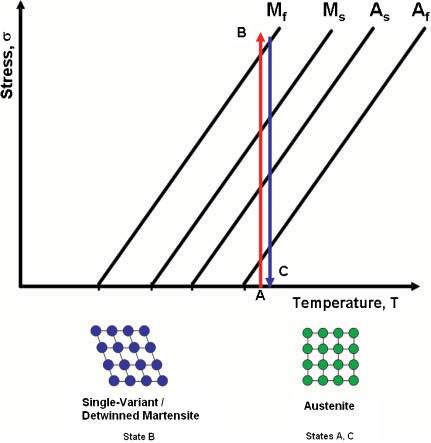
\includegraphics[scale=0.4]{img/StressTransformation.png}
	\caption{Cambio de las temperaturas características con la aplicación de tensión.}
	\label{TvsS}
\end{figure}

\subsubsection{Termodinámica de la transformación}
Las transformaciones martensíticas son transformaciones de fase de primer orden sin difusión. Por no tener difusión, no hay cambios de composición y entonces el sistema termodinámico es un sistema monocomponente con dos fases sólidas de diferentes estructuras.\cite{Santamarta}

\begin{figure}
	\centering
	\includegraphics[scale=0.7]{img/Termo.eps}
	\caption{Fracción transformada ($\xi$) y energía libre de Gibbs de ambas fases como función de la temperatura en los casos: si la transformación sucediera a la temperatura de equilibrio termodinámico (a) y (b), si sólo hubiera trabajo de fricción (c) y (d), si hubiera tanto trabajo de fricción como trabajo elástico (e) y (f).} 
	\label{Gibbs}
\end{figure}

Se denomina termoelástica a una transformación martensítica cuando la deformación que produce la transformación es absorbida en forma elástica por la matriz (en este caso particular la austenita, $A$) que rodea a la martensita ($M$), de forma que existe un equilibrio termoelástico local entre una energía de origen químico y una de origen elástico que controla el avance de la transformación. La fuerza motriz de la transformación es la diferencia de energías libres químicas o estructurales entre las fases matriz y martensita, esto es:

\begin{equation}
\Delta G^{A \rightarrow M}_q = G^M_q - G^A_q
\end{equation} 

En el caso ideal, la transformación sucedería a la temperatura de equilibrio termodinámico $T_0$, la cual se define como la temperatura en la cual la diferencia de energía libre química entre ambas fases es cero ($\Delta G^{A \rightarrow M}_q = 0$). Esta transformación sería termodinámicamente reversible y es esquematizada en la Figura \ref{Gibbs}(a) y \ref{Gibbs}(b), en donde se observa que la fase estable a temperatura mayor a $T_0$ sería la austenita, mientras que a temperaturas menores a $T_0$ la fase estable sería la martensítica. Sin embargo, como ya vimos, la transformación comienza en $M_s$  ($< T_0$) y se extiende en un intervalo de temperaturas hasta $M_f$  $(< M_s)$. Esto se debe a que el sistema necesita una energía suplementaria $\Delta G_q$ para compensar las energías de origen no químico que se oponen a la transformación cuando esta ocurre. Las contribuciones más importantes al término no químico son: un término disipativo que se manifiesta experimentalmente por la presencia de histéresis ver Figura \ref{Gibbs}(c) y \ref{Gibbs}(d)) y la deformación elástica entre la fase matriz y la martensita, la cual se almacena durante la transformación (ver Figura \ref{Gibbs}(e) y \ref{Gibbs}(f)). El término disipativo incluye el trabajo de fricción generado en el movimiento de las interfases e interacción de las mismas con otras variantes y/o defectos. El término elástico, por otra parte, proviene de la acomodación de los cambios de forma y volumen asociados a la transformación\cite{Wollants1993}.

Debido al trabajo de fricción y el proceso de acumulación de energía elástica, la transformación martensítica consiste en un proceso irreversible desde el punto de vista de la termodinámica, a pesar de que es un proceso mecánicamente reversible. Por lo tanto, la diferencia de energía libre química entre ambas fases se relaciona con el trabajo de fircción ($W_{fric}$) y el trabajo elástico ($W_{elast}$) mediante la siguiente ecuación \footnote{Esta relación se deduce desde el primer y segundo principio de la termodinámica, tomando como convención de signos que el calor absorbido por el sistema y el trabajo realizado sobre el sistema son ambos positivos.}\cite{Isola2020}:

\begin{equation}
\label{GibbsEnergyEquation}
	- \Delta G_{q}^{A \leftrightarrow M} \geq W_{elast} + W_{fric}
\end{equation}

En una transformación inducida térmicamente, $\Delta G_{q}^{A \leftrightarrow M}$ siempre es menor a cero (ver Figura \ref{Gibbs}), mientras que el trabajo de fricción siempre es positivo (ya que es realizado sobre el volumen que transforma), por lo cual se opone al cambio de fase y es el responsable del efecto de histéresis en la transformación, el trabajo elástico es negativo durante la retransformación, por lo cual ayudará a está última. Este trabajo elástico es el responsable de que la transformación se desarrolle en el rango de temperatura definido por las temperaturas $M_s$ y $M_f$ (ver Figura \ref{Gibbs}(e) y \ref{Gibbs}(f)).


\subsubsection{Efectos de memoria de forma y superelasticidad como consecuencias de la transformación}

El proceso de memoria de forma comienza a una temperatura $T>A_f$. La forma que tenga el material en este punto es la que será ``recordada''. Luego, se enfría sin una tensión externa hasta una temperatura $T<M_f$. En este enfriamiento, como ya vimos, se produce la transformación directa de austenita a martensita, formándose la martensita de manera que la energía del sistema se minimice. Al no haber tensiones externas, la martensita se acomoda de tal manera que la forma macroscópica del material no cambie.

Siendo la estructura del material la martensita, se aplica un esfuerzo creciente para deformar la aleación. Tanto la deformación elástica de la martensita como la reorientación de las variantes formadas durante el enfriamiento dan lugar a esta deformación. Como estas variantes se mueven con facilidad, se acomodan para concordar con el esfuerzo aplicado. Aún así, si la deformación es muy grande, existe la posibilidad que haya una deformación plástica y el proceso no sea completamente reversible. Una vez relajado el esfuerzo, el material conserva una deformación residual.

Finalmente, al calentarse la aleación a una temperatura $T>A_f$ se da la transformación inversa (martensita a austenita). De esta manera recupera la aleación su forma original, perdiéndose la deformación residual. En la Figura \ref{3DGraph} puede verse esquemáticamente este proceso.

\begin{figure}[H]
	\centering
	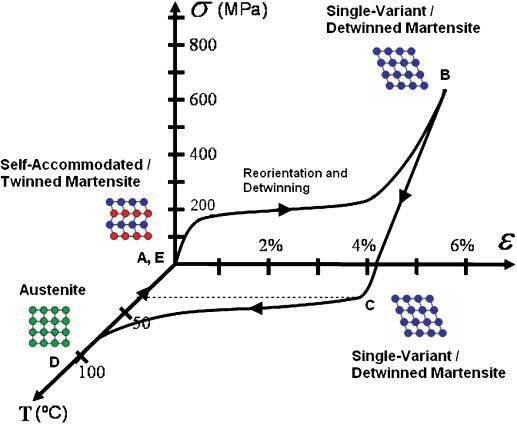
\includegraphics[scale=0.5]{img/3dCycle.png}
	\caption{Diagrama del efecto de memoria de forma en función de tensión y temperatura.}
	\label{3DGraph}
\end{figure}


Se denomina superelasticidad cuando se induce la transformación martensítica por tensión, a una temperatura mayor a $A_f$. Aplicando tensión al material en austenita, empieza a deformar elásticamente hasta la tensión $\sigma^{p \rightarrow m}$ valor a partir del cual comienza la transformación martensítica.

Al retirarse la tensión, ocurre la transformación inversa, habiendo, al igual que en el caso de memoria de forma, histéresis.


\subsection{Diagrama de fases de la familia $Ni-Ti$}
\label{PhaseDiagramSection}

En la Figura \ref{PhaseDiagram} puede verse el diagrama de fases de la aleación binaria. Por debajo de los $650 ^\circ C$ no existe un conocimiento claro del diagrama de equilibrio, aunque se acepta de manera general que la zona de estabilidad de la fase austenita es sumamente estrecha (entre 50.0 y 50.5 \% at. $Ni$) y que por debajo de $650^\circ C$ es una fase metaestable. Sólo la fase $NiTi$ es la que presenta una transformación martensítica y, por lo tanto, es la única con el efecto de memoria de forma.

Viendo el diagrama es fácil poder apreciar cuales son las fases que acompañaran al $NiTi$ cuasi-equiatómico (austenita B2). El $Ti_2Ni$ aparece cuando el contenido de $Ti$ es mayor que el de $Ni$. Es importante aclarar que es difícil distinguir esta fase del óxido $Ti_4Ni_2O$ debido a que sus parámetros de red son casi idénticos (la diferencia es menor al 1\%). Por otra parte, cuando el contenido de $Ni$ es mayor, la única fase estable que acompaña al $NiTi$ es $TiNi_3$.

\begin{figure}[H]
	\centering
	\subfloat[Diagrama completo]{
  		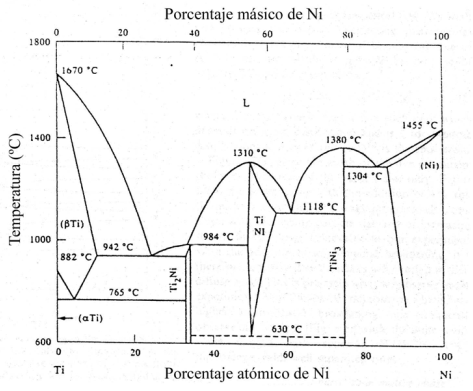
\includegraphics[width=70mm]{img/NiTiPhaseDiagramCompleteSpanish.png}
	}
	\subfloat[Diagrama centrado en $NiTi$]{
  		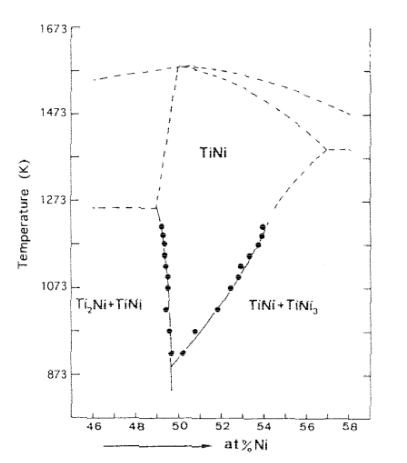
\includegraphics[width=70mm]{img/NiTiphasediagram.png}
	}
	\caption{Diagrama de fases de la aleación $Ni-Ti$.}
	\label{PhaseDiagram}
\end{figure}

La transformación martensítica, como ya se ha mencionado, es una transformación de estado sólido entre dos fases cristalinas. Estas fases han sido objeto de un estudio extensivo desde un punto de vista cristalográfico. En el caso de la aleación binaria $NiTi$ y, en general, en las aleaciones de la familia $Ni-Ti$, se pueden distinguir la fase austenita (B2) y varios tipos de martensita, entre las que podemos destacar la que se conoce como fase R, una fase monoclínica (B19’) y una ortorrómbica (B19).

Cuando se adiciona un tercer aleante aparecen nuevas fases. En el caso de la adición de $Zr$ en detrimento del $Ti$, pueden destacarse las siguientes fases: $NiZr$, la fase $\lambda$ en composiciones pobres en $Ni$ ($Ni < 50\%$) y la fase H en composiciones ricas en $Ni$ ($Ni > 50\%$). A continuación, se realiza una breve descripción de dichas fases.

\subsubsection{Fase B2}
La fase B2 es la correspondiente a la austenita en las aleaciones casi-equiatómicas de $NiTi$. En la Figura \ref{B2phase} puede verse su estructura. Es una estructura cúbica simple ordenada cuyos átomos del motivo están en las posiciones 000 y $\frac{1}{2}\frac{1}{2}\frac{1}{2}$. Esta estructura también es conocida como CsCl.
\begin{figure}[H]
	\centering
	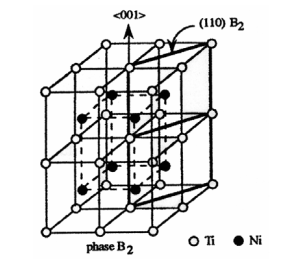
\includegraphics[scale=0.5]{img/B2Phase.png}
	\caption{Estructura de la fase B2.}
	\label{B2phase}
\end{figure}

A temperatura ambiente esta fase es metaestable. Se la obtiene desde temperaturas mayores a $650 ^\circ C$ realizando un templado hasta la temperatura ambiente.

Los parámetros de red que se pueden encontrar en la literatura pueden variar significativamente, especialmente a causa de los elementos adicionales a la aleación binaria y la cantidad de los mismos. Sin embargo, incluso para la aleación binaria, se pueden hallar valores dispares, generalmente comprendidos entre 2.9 y 3.1 \AA \cite{Santamarta}.

\subsubsection{Fase R}
La fase R, es una estructura martensítica correspondiente a una distorsión
ortorrómbica de la malla cúbica (B2) en la dirección $<$111$>$, como se ve en la Figura \ref{RPhase}, aunque lo estándar es describirla usando una red hexagonal.
\begin{figure}[H]
	\centering	
	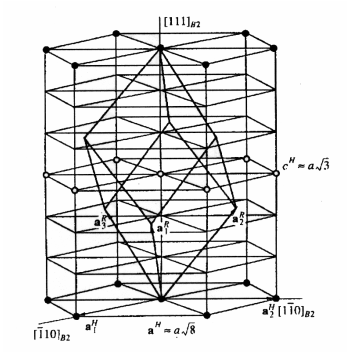
\includegraphics[scale=0.5]{img/RPhase.png}
	\caption{Estructura de la fase R.}
	\label{RPhase}
\end{figure}

Esta fase aparece sólo bajo ciertas condiciones antes de la transformación a la fase B19'. Este fenómeno fue interpretado muchas veces como un efecto previo a la transformación, pero actualmente lo aceptado es que es una transformación martensítica de la fase matriz B2 a las fase R, que posee una estructura distinta. Los motivos para este análisis son los siguientes:
\begin{itemize}
	\item Láminas martensíticas de la fase R son claramente observadas por microscopía electrónica.
	\item La transformación directa B2 $\rightarrow$ B19' sólo ocurre en ciertas condiciones.
	\item En este proceso también se observan los efectos de memoria de forma y súper elasticidad.
\end{itemize}


Esta fase se ha encontrado en aleaciones ternarias, en las cuales parte del $Ni$ es sustituido por $Al$, $Fe$ o $Co$. Se ha hallado que en  aleaciones binarias de $NiTi$ la transformación B2 $\rightarrow$ R $\rightarrow$ B19', que compite con B2 $\rightarrow$ B19', puede favorecerse con ciclado térmico, envejecimiento a $T \approx 400 ^\circ C$ y tratamiento de calor luego de trabajo en frío para generar estructuras dislocadas \cite{Santamarta}\cite{ThinFilm}\cite{TiNi}. 


\subsubsection{Fase B19'}
La fase martensítica B19' es una estructura monoclínica. Esta es la fase que se conoce como martensita. En la Figura \ref{B19pPhase} se muestra su estructura. Puede haber hasta 24 variantes, según en qué dirección sea la deformación de la fase B2\cite{Santamarta}.
\begin{figure}[H]
	\centering
	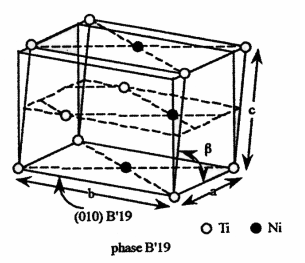
\includegraphics[scale=0.5]{img/B19pPhase.png}
	\caption{Estructura de la fase B19'.}
	\label{B19pPhase}
\end{figure}

\subsubsection{Fase $Ti_2Ni$ y $Ti_4Ni_2O$}
\label{Ti2Ni}
Los parámetros de estas fases son muy similares, por lo cual resulta difícil distinguirlas entre sí. La fase $Ti_2Ni$ aparece en composiciones pobres en $Ni$, mientras que la fase $Ti_4Ni_2O$ aparece por la presencia de oxígeno en algún momento del proceso de elaboración de la aleación. Ambas fases se corresponden con una estructura FCC, con grupo espacial $Fd3m$ (número 227) y sus parámetros de red son cercanos a 11,3 $\AA$ \cite{ShapeMemoryMaterials}.

\subsubsection{Fase $NiZr$}
La fase $NiZr$ tiene una estructura ortorrómbica y su grupo espacial es $Cmcm$ (número 63) \cite{Kirkpatrick1962}.

\subsubsection{Fase $\lambda$}
La fase $\lambda$ es una solución sólida ternaria de $Ti$, $Ni$ y $Zr$ con una estructura tipo C14 Laves, la cual es una fase hexagonal y su grupo espacial es $P6_3/mmc$ (número 194). En el trabajo \cite{Bououdina2003}, a través de refinamiento de difracción de neutrones, se reporta la fórmula química $Ni_{0,91}Ti_{1,21}Zr_{0,88}$ para esta fase.

\subsubsection{Fase H}
La fase H tiene una estructura ortorrómbica y su grupo espacial es $Fddd$ (número 70) \cite{Yang2013} \cite{Santamarta2013}. Se encuentra en composiciones ricas en $Ni$ cuando a la aleación binara de $NiTi$ se le agrega $Zr$ o $Hf$. Su estructura se construye como una superestructura de la fase B2, desde la recombinación de los átomos $Zr$/$Hf$ y $Ti$ en su subred, con un posterior desplazamiento de los átomos\cite{Evirgen2018}. La composición de esta fase es rica en $Ni$ y en el tercer aleante ($Zr$/$Hf$), mientras que resulta pobre en $Ti$. Las estructuras de la fase H y la fase matriz B2 tiene un alto nivel de acuerdo, lo cual permite una completa coherencia caracterizada por un ajuste perfecto del plano de la interfase austenita-precipitado\cite{Evirgen2018}.


\subsection{Magnetrón sputtering}
La deposición física por sputtering es una deposición física de vapor usada para generar películas delgadas. Este proceso consiste en la emisión de material desde un blanco para depositarlo sobre un sustrato. 

 Los átomos o moléculas del material del blanco son arrancados mediante colisiones con los átomos ionizados de un gas inerte, típicamente $Ar$. Las partículas abandonan la superficie del target como partículas libres o como una combinación química con las partículas del gas ionizado para luego despositarse sobre una superficie cercana.  Esta ``superficie cercana'' es justamente un sustrato dedicado a dicha finalidad.
 
Para generar llevar el gas inerte al estado de plasma es necesario alto vacío $\approx 1 mTorr$ y un voltaje DC de al menos 500 V. Para aumentar la velocidad de deposición, se aplica un campo magnético alrededor de los blancos. Eso provoca que los electrones orbiten dentro del plasma, ahora concentrado sobre los blancos, y aumenten la cantidad de choques por unidad de tiempo. Es este campo lo que le da el nombre de \textit{Magnetrón sputtering}\cite{Malvasio}\cite{ThinFilm}. En la Figura \ref{sputter} puede verse esquemáticamente cómo es la disposición experimental del proceso.

\begin{figure}[H]
	\centering
	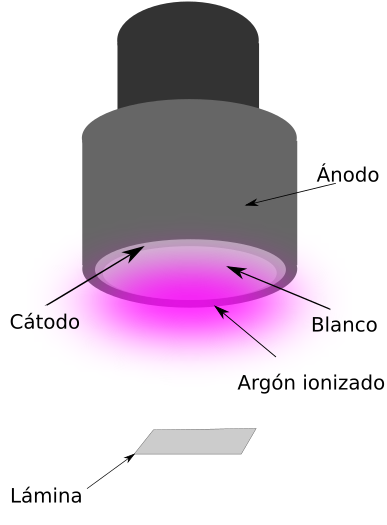
\includegraphics[scale=0.5]{img/SchemaDeposition.png}
	\caption{Esquema del magnetrón sputtering.}
	\label{sputter}
\end{figure}

\subsection{Cristalización}

La cristalización es un proceso importante en la fabricación de láminas delgadas de $NiTi$, ya que es la microestructura la que dicta las propiedades macroscópicas del material y dicha microestructura es fuertemente influenciada por la forma en que se crea el material. A diferencia de la fusión de un material, la cristalización no sucede a una temperatura definida, sino que depende tanto del tiempo como de la temperatura.

La deposición por sputtering debe ser hecha en manera muy cuidadosa, ya que las láminas de $NiTi$ producidas por sputtering a temperatura ambiente son sólidos amorfos. Para obtener las fases deseadas, es importante planificar y controlar los parámetros de los tratamientos térmicos. Para ello deben tenerse en cuenta factores como la temperatura y la energía de activación del proceso de cristalización.

\subsubsection{Ecuación de Johnson-Mehl}

 El proceso de cristalización ocurre por nucleación y crecimiento. La nucleación es la formación del primer volumen de la nueva fase dentro del material de partida. El crecimiento de estos núcleos sucede por la transferencia de átomos a través de la interfase, desde la original hacia las zonas nucleadas. Este proceso continúa hasta que toda la muestra ha cristalizado. En la Figura \ref{cristalization} se muestra esquemáticamente este proceso.
 \begin{figure}[H]
 	\centering
	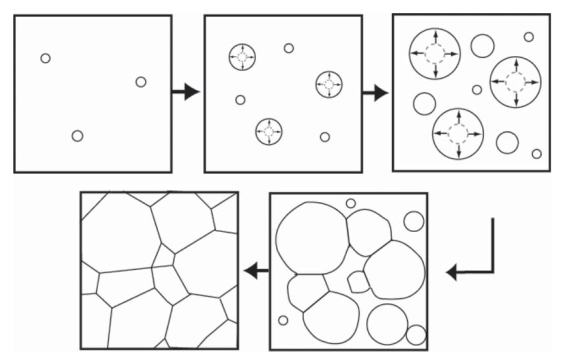
\includegraphics[scale=0.5]{img/cristalization.png}
 	\caption{Esquema del proceso de nucleación y crecimiento.}
	\label{cristalization}
\end{figure} 

Para comenzar el análisis de la transformación, supondremos que la transformación es isotérmica.

Supongamos que la muestra tiene un volumen total $V$, y el volumen transformado de una fase inicial $\alpha$ a otra fase $\beta$ es $V_\beta$. Intuitivamente podemos imaginar que la fracción de muestra cristalizada en función del tiempo, $X(t) = \frac{V_\beta (t)}{V}$ tendrá un carácter sigmoidal, mostrado esquemáticamente en la Figura \ref{cvst}.

 \begin{figure}[H]
 	\centering
	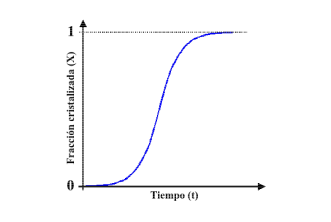
\includegraphics[scale=1]{img/cristalization_vs_tiempo.png}
 	\caption{Porcentaje de muestra transformado en función del tiempo.}
	\label{cvst}
\end{figure} 

La rapidez con que aparecen nuevas partículas transformadas por unidad de volumen se llama velocidad de nucleación y se denota por $I$. Análogamente, se llama velocidad de crecimiento a la velocidad con que aumenta el radio de los núcleos formados y se denota por $\Gamma$.

Para comprender cómo cristaliza la muestra en su totalidad, empecemos por
considerar el tamaño de una región individual ya en fase $\beta$, es decir, ya cristalizada. La región se forma en un tiempo de incubación $t=\tau$, y luego crece en forma continua. Si la fase inicial y final tienen la misma composición, en la mayor parte de los casos, se observa experimentalmente que cualquier dimensión de la región transformada es una función lineal del tiempo \cite{Transformations2002}.

Para facilitar el análisis asumiremos una velocidad de crecimiento isotrópica $\Gamma$, lo que implica que las regiones transforman con simetría esférica. Hay que destacar que no se pierde mucha generalidad con esta aproximación, aunque este no suela ser el caso. Con estás hipótesis, el volumen $v_\tau$ de una región que transformó en un tiempo de incubación es:
\begin{equation}
	v_\tau = \frac{4}{3}\pi \Gamma^3(t-\tau)^3
\end{equation}

El número de nuevas regiones en la fase $\beta$ nucleadas en un intervalo de tiempo entre $\tau$ y $\tau + d\tau$ es $IV_\alpha d\tau$. Entonces, el volumen transformado en un tiempo t, producto de dichas regiones nucleadas es $v_\tau IV_\alpha d\tau$. Al inicio de la transformación, podemos asumir que la velocidad de nucleación $I$ y la de crecimiento $\Gamma$ son constantes y que como $V_\beta << V_\alpha$ entonces $V_\alpha \approx V$, resulta:

\begin{equation}
\label{integral}
	V_\beta = \frac{4}{3}\pi V \int_{\tau = 0}^{t} I\Gamma^3(t-\tau)^3d\tau
\end{equation}

Esta función, llamada función de Johnson-Mehl, da como resultado que la fracción transformada en función del tiempo es:
\begin{equation}
\label{eq1}
	X_e(t) = \frac{V_\beta (t)}{V} = \frac{\pi}{3}\Gamma^3 I t^4
\end{equation}

En esta ecuación la fracción transformada tiende a infinito con el tiempo. El error no es sorprendente ya que en la hipótesis considerada la transformación recién comenzaba, y de hecho, experimentalmente la Ecuación \ref{eq1} describe bien la fracción transformada en el $t \approx 0$. El subíndice $e$ es porque esta fracción suele llamarse fracción cristalizada extendida.

En un análisis más exacto, se debe considerar la interferencia entre las regiones transformadas durante el proceso de crecimiento. Al chocar entre sí dos regiones transformadas, puede ocurrir una de tres cosas:
\begin{itemize}
\item Las regiones pueden unirse y formar una única región.
\item Pueden tocarse y seguir creciendo como si nunca hubieran interferido.
\item Pueden formar una interfase en la que el crecimiento frena, aunque siga en otras partes.
\end{itemize}

De todas estas posibilidades, la última es la que ocurre en una transformación de estado sólido.

Anteriormente se asumió en forma implícita que la nucleación ocurre en forma aleatoria, aunque esto no necesariamente es cierto, la hipótesis aún puede ser aplicada. Lo que en verdad sucede es que la nucleación ocurre en sitios preferenciales de la muestra. Sin embargo, dividiendo la muestra en pequeños elementos de volumen, cada elemento contiene muchos de estos sitios preferenciales, con lo cual puede asumirse que cada uno de estos elementos tiene la misma probabilidad de nucleación. Como esta nucleación es igualmente probable en todas partes, cuanto mayor sea la fracción cristalizada, mayor es la probabilidad que $dX_e$ sea de lo ya transformado. Describiendo entonces la fracción cristalizada real con respecto a la fracción cristalizada anterior queda:
\begin{equation}
 dX = (1 - X)dX_e
\end{equation}
La solución de está ecuación diferencial es:
\begin{equation}
	X(t)=1-e^{-\frac{\pi}{3}V^3 I t^4}
\end{equation}
Esta ecuación se conoce como ecuación de Johnson-Mehl y describe correctamente la curva de la Figura \ref{cvst}. Esta ecuación mantiene el comportamiento proporcional a $t^4$ para tiempos chicos, pero satura en $X = 1$ para tiempos grandes.

\subsubsection{Modelo de Avrami}
En general, la velocidad de nucleación $I$ no es constante. Para corregir este hecho, Avrami consideró que la nucleación sólo ocurre en sitios preferenciales de la muestra que se van agotando con el tiempo. Sea $N_0$ los sitios iniciales de nucleación por unidad de volumen en la muestra, luego de un tiempo t tenemos:
\begin{equation}
	N(t) = N_0e^{-\nu t}
\end{equation}
donde $\nu$ es la velocidad con la que un sitio se convierte en núcleo. Luego, la velocidad de nucleación por unidad de volumen es:
\begin{equation}
	I = -\frac{dN}{dt} = N_0\nu e^{-\nu t} = N\nu
\end{equation}
Sustituyendo esta fórmula en la Ecuación \ref{integral} e integrando por partes queda:
\begin{equation}
	X = 1-exp \left\lbrace 8\pi N_0\frac{\Gamma^3}{\nu^3} \left[ e^{-\nu t} -1+\nu t -\nu^2t^2/2 + \nu^3 t^3/6 \right] \right\rbrace
\end{equation}

Para valores chicos de $\nu t$ se obtiene nuevamente la ecuación de Johnson-Mehl, pero para valores grandes de $\nu t$ resulta:
\begin{equation}
	X = 1 - exp\left\lbrace -\frac{4}{3} \pi N_0 \nu^3 t^3 \right\rbrace
\end{equation}
En general la fracción cristalizada en función del tiempo sigue la ecuación:

\begin{equation}
	X = 1 - e^{-(kt)^n}
\end{equation}

donde $n$ es el exponente de Avrami y $k$ una constante dependiente de la velocidad de nucleación y crecimiento.

	El exponente de Avrami generalmente toma valores entre 1.5 y 4, y en casos de nucleación tridimensional se restringe a valores entre 3 y 4. Esto debería cubrir los casos en los que la velocidad de nucleación $I$ es una función decreciente en el tiempo, hasta el caso límite ($n = 4$) en que es constante. En el caso de láminas delgadas, el crecimiento en el espesor finaliza rápidamente, con lo cual el proceso es esencialmente bidimensional y $n$ toma valores entre 2 y 3, siendo 3 el caso límite de velocidad de nucleación constante. 
	
Como los procesos de nucleación y crecimientos son procesos activados térmicamente, la constante k puede ser descripta como:
\begin{equation}
\label{kvalue}
	k=fe^{-\frac{E_c}{RT}}
\end{equation}

donde $f$ es el llamado factor de frecuencia y $E_c$ la energía de activación.
La cristalización puede ser descripta completamente si se conocen los valores de $n$, $E_c$ y f. Estos parámetros normalmente se hallan midiendo la fracción cristalizada en función del tiempo para procesos isótermicos y ajustando la ecuación convenientemente.

La energía de activación de la cristalización puede usarse para describir la estabilidad térmica de una fase, donde mayores números se corresponden con mayores valores de estabilidad.

\subsubsection{Relación de Kissinger}
Para lograr medir la energía de activación en procesos térmicamente activados, Kissinger desarrolló una formulación teórica sencilla para describir los experimentos en los cuales la temperatura aumenta a ritmo constante. Esta formulación se basa en que la probabilidad de que una región transforme es la misma para todas las partes del volumen sin transformar, es decir que la transformación es homogénea. Entonces, el volumen transformado en un intervalo de tiempo es proporcional al volumen que quedaba en la fase original al comienzo de dicho intervalo, esto es $dV_\beta = k V_\alpha dt$. Esto permite expresar la velocidad de transformación en función del porcentaje transformado mediante la siguiente ecuación diferencial:
\begin{equation}
	\dot{X} = k(1-X)
\end{equation}
cuya solución es:
\begin{equation}
	X(t) = 1 - e^{-kt}
\end{equation}
que es en definitiva un caso particular del modelo de Avrami en el cual $n=1$.
Suponiendo que el aumento de temperatura ocurre en forma constante, como es el caso de un proceso de calorimetría diferencial de barrido, se tiene que:
\begin{equation}
	T(t) = T_0+\alpha t
\end{equation}
donde $T_0$ es la temperatura inicial y $\alpha$ la velocidad de calentamiento. El máximo de la velocidad de reacción $\dot{X}$ ocurre en el pico del barrido, y en la temperatura de este pico ($T_p$) se tiene que $\ddot{X} = 0$.

Con estas consideraciones, y recordando el valor de k de la Ecuación \ref{kvalue} se llega a la ecuación:
\begin{equation}
	fe^{-\frac{E_c}{RT}} = \frac{\alpha E_c}{R T_p^2}
\end{equation}

Aplicando logaritmo natural miembro a miembro para simplificar la expresión se obtiene la relación de Kissinger:
\begin{equation}
	ln(\frac{\alpha}{R T_p^2}) = -\frac{E_c}{RT_p} + cte
\end{equation}

Con los diversos valores de $T_p$ obtenidos de barridos a distintas velocidades $\alpha$ puede graficarse $ln(\frac{\alpha}{R T_p^2})$ vs $T_p^{-1}$, y de la pendiente de esta recta puede obtenerse el valor de la energía de activación, $E_c$.

\subsubsection{Relación de Augis-Bennet}
Para conservar el modelo de Avrami en un proceso a temperatura variable, Augis y Bennet propusieron un modelo alternativo al de Kissinger. Este considera que el proceso es aproximable por una sucesión de pasos isotérmicos.
De la Ecuación \ref{kvalue} y de considerar a la temperatura como una función lineal en el tiempo, podemos definir:
\begin{equation}
	u = k\: t = f\: t\: exp \left\lbrace -\frac{E_c}{R(T_0 + \alpha t)} \right\rbrace
\end{equation}

Esto permite reescribir el modelo de Avrami como:
\begin{equation}
	X = 1-e^{-u^{n}}
\end{equation}
de donde sale que:
\begin{equation}
	\dot{X} = \dot{u}\: n\: u^{n-1}(1-X)
\end{equation}
Considerando una vez más que el máximo de la velocidad de la reacción coincide con el pico del barrido, vuelve a suceder que $\ddot{X}(T_p) = 0$. En este modelo se llega a la siguiente expresión:
\begin{equation}
	f^n exp \left\lbrace -\frac{n E_c}{RT_p} \right\rbrace = (\frac{\alpha}{T_p - T_0})^n
\end{equation}

Aplicando logaritmo natural a esta expresión se obtiene la relación de Augis Bennet:
\begin{equation}
	ln(\frac{\alpha}{T_p - T_0}) = -\frac{n E_c}{RT_p} + cte
\end{equation}
Donde la forma de hallar el valor de $E_c$ es similar a la de Kissinger, a partir de la pendiente de la gráfica $ln(\frac{\alpha}{T_p - T_0})$.

\newpage

\section{Técnicas experimentales}

\subsection{Deposición por magnetrón sputtering}
Para realizar la deposición de las láminas delgadas se usaron 3 magnetrones modelo MeiVac MAK-130-V, los cuales pueden verse en la Figura \ref{magnetrones}. Los magnetrones están construidos de manera que su superficie exterior, de acero inoxidable, funciona como ánodo, mientras que el blanco del material a depositar hace el papel de cátodo. Además, en su interior poseen dos imanes concéntricos que permiten la concentración de la descarga en un anillo sobre la superficie del blanco. Entre estos imanes se encuentra una serie de cilindros huecos aislantes y un anillo de cobre conectado a la fuente de tensión y al sistema de circulación de agua, que actúa como refrigerante durante la experiencia.

A los blancos no magnéticos se les suelda por punto una arandela de hierro niquelada, la cual permite que se acoplen magnéticamente al magnetrón y mediante una pasta conductora se asegura el contacto térmico y eléctrico con el anillo de cobre. Los blancos usados para generar las láminas delgadas fueron de titanio, níquel y zirconio ($99,99$ \% de pureza en todos los casos).


Los magnetrones están colocados en la tapa superior de la cámara de  deposición, construida en acero inoxidable, la cual se muestra en la Figura \ref{camara}. Dicha cámara posee una ventana de cuarzo para poder ver en su interior, sin embargo al avanzar la deposición dicha ventana se contamina, imposibilitando así la visión dentro de la cámara.

\begin{figure}[H]
	\centering
	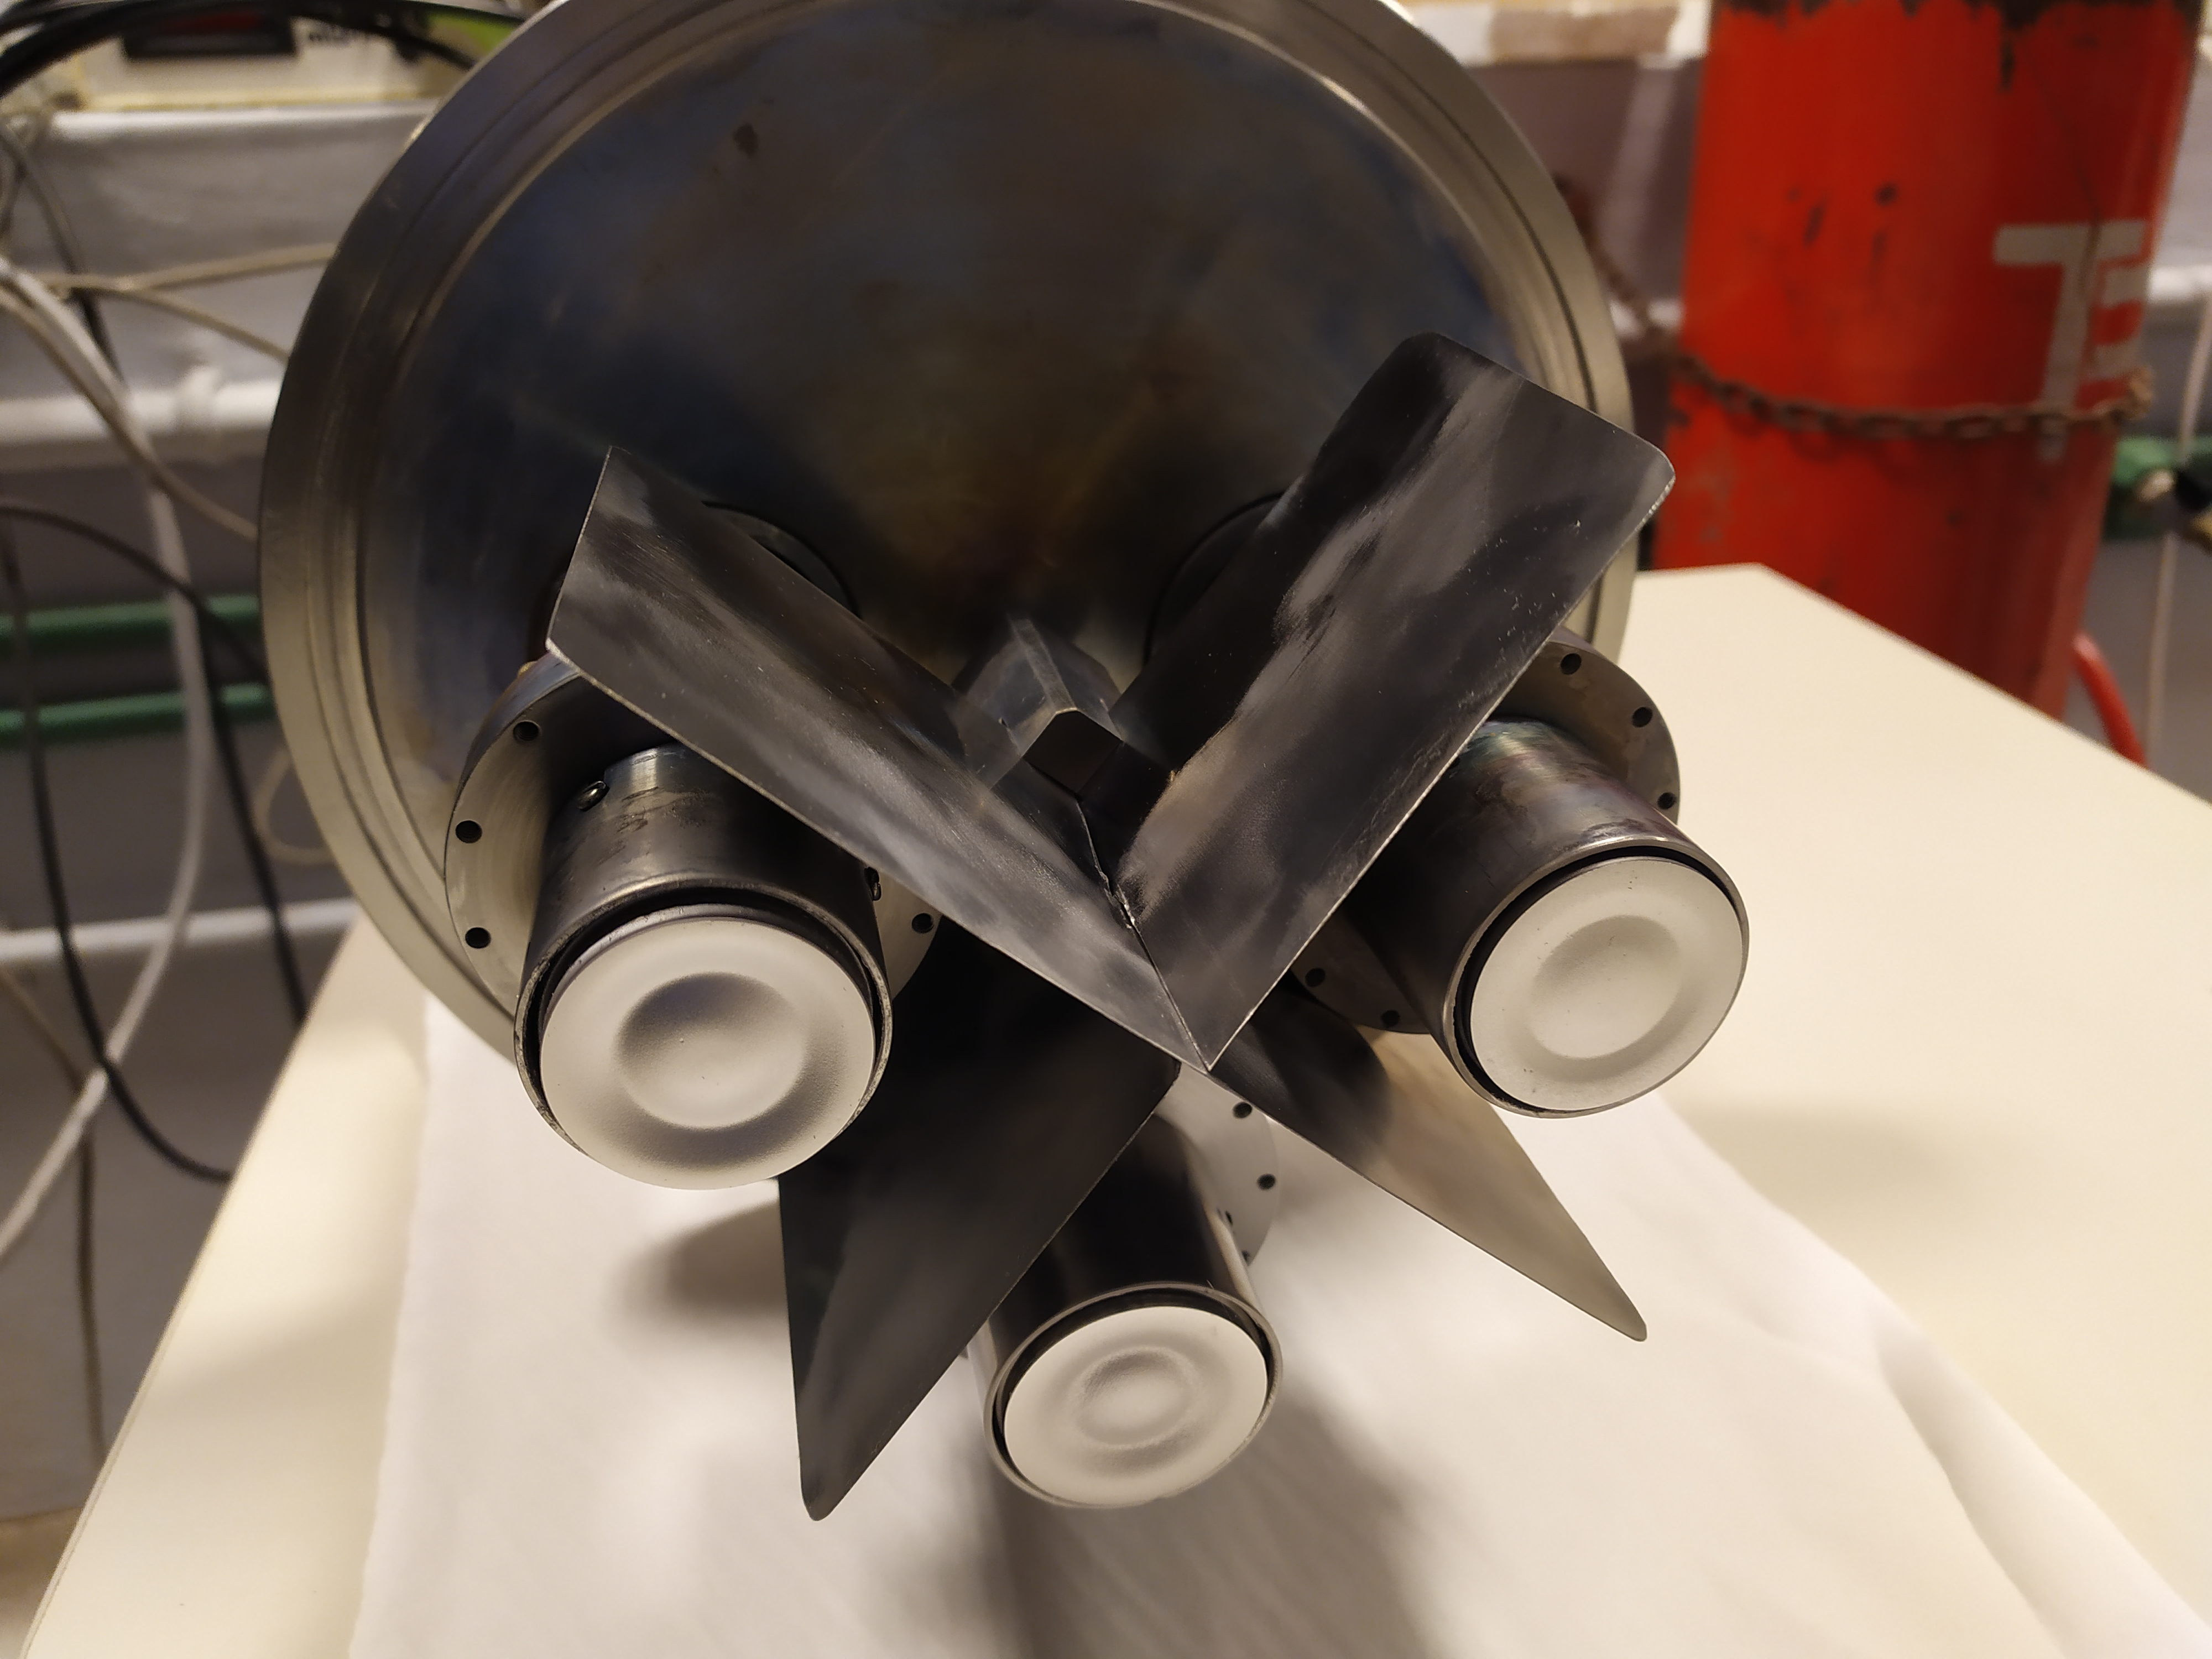
\includegraphics[scale=0.1]{img/magnetrones.jpg}
	\caption{Magnetrones empleados durante las deposiciones.}
	\label{magnetrones}
\end{figure}

\begin{figure}[H]
	\centering
	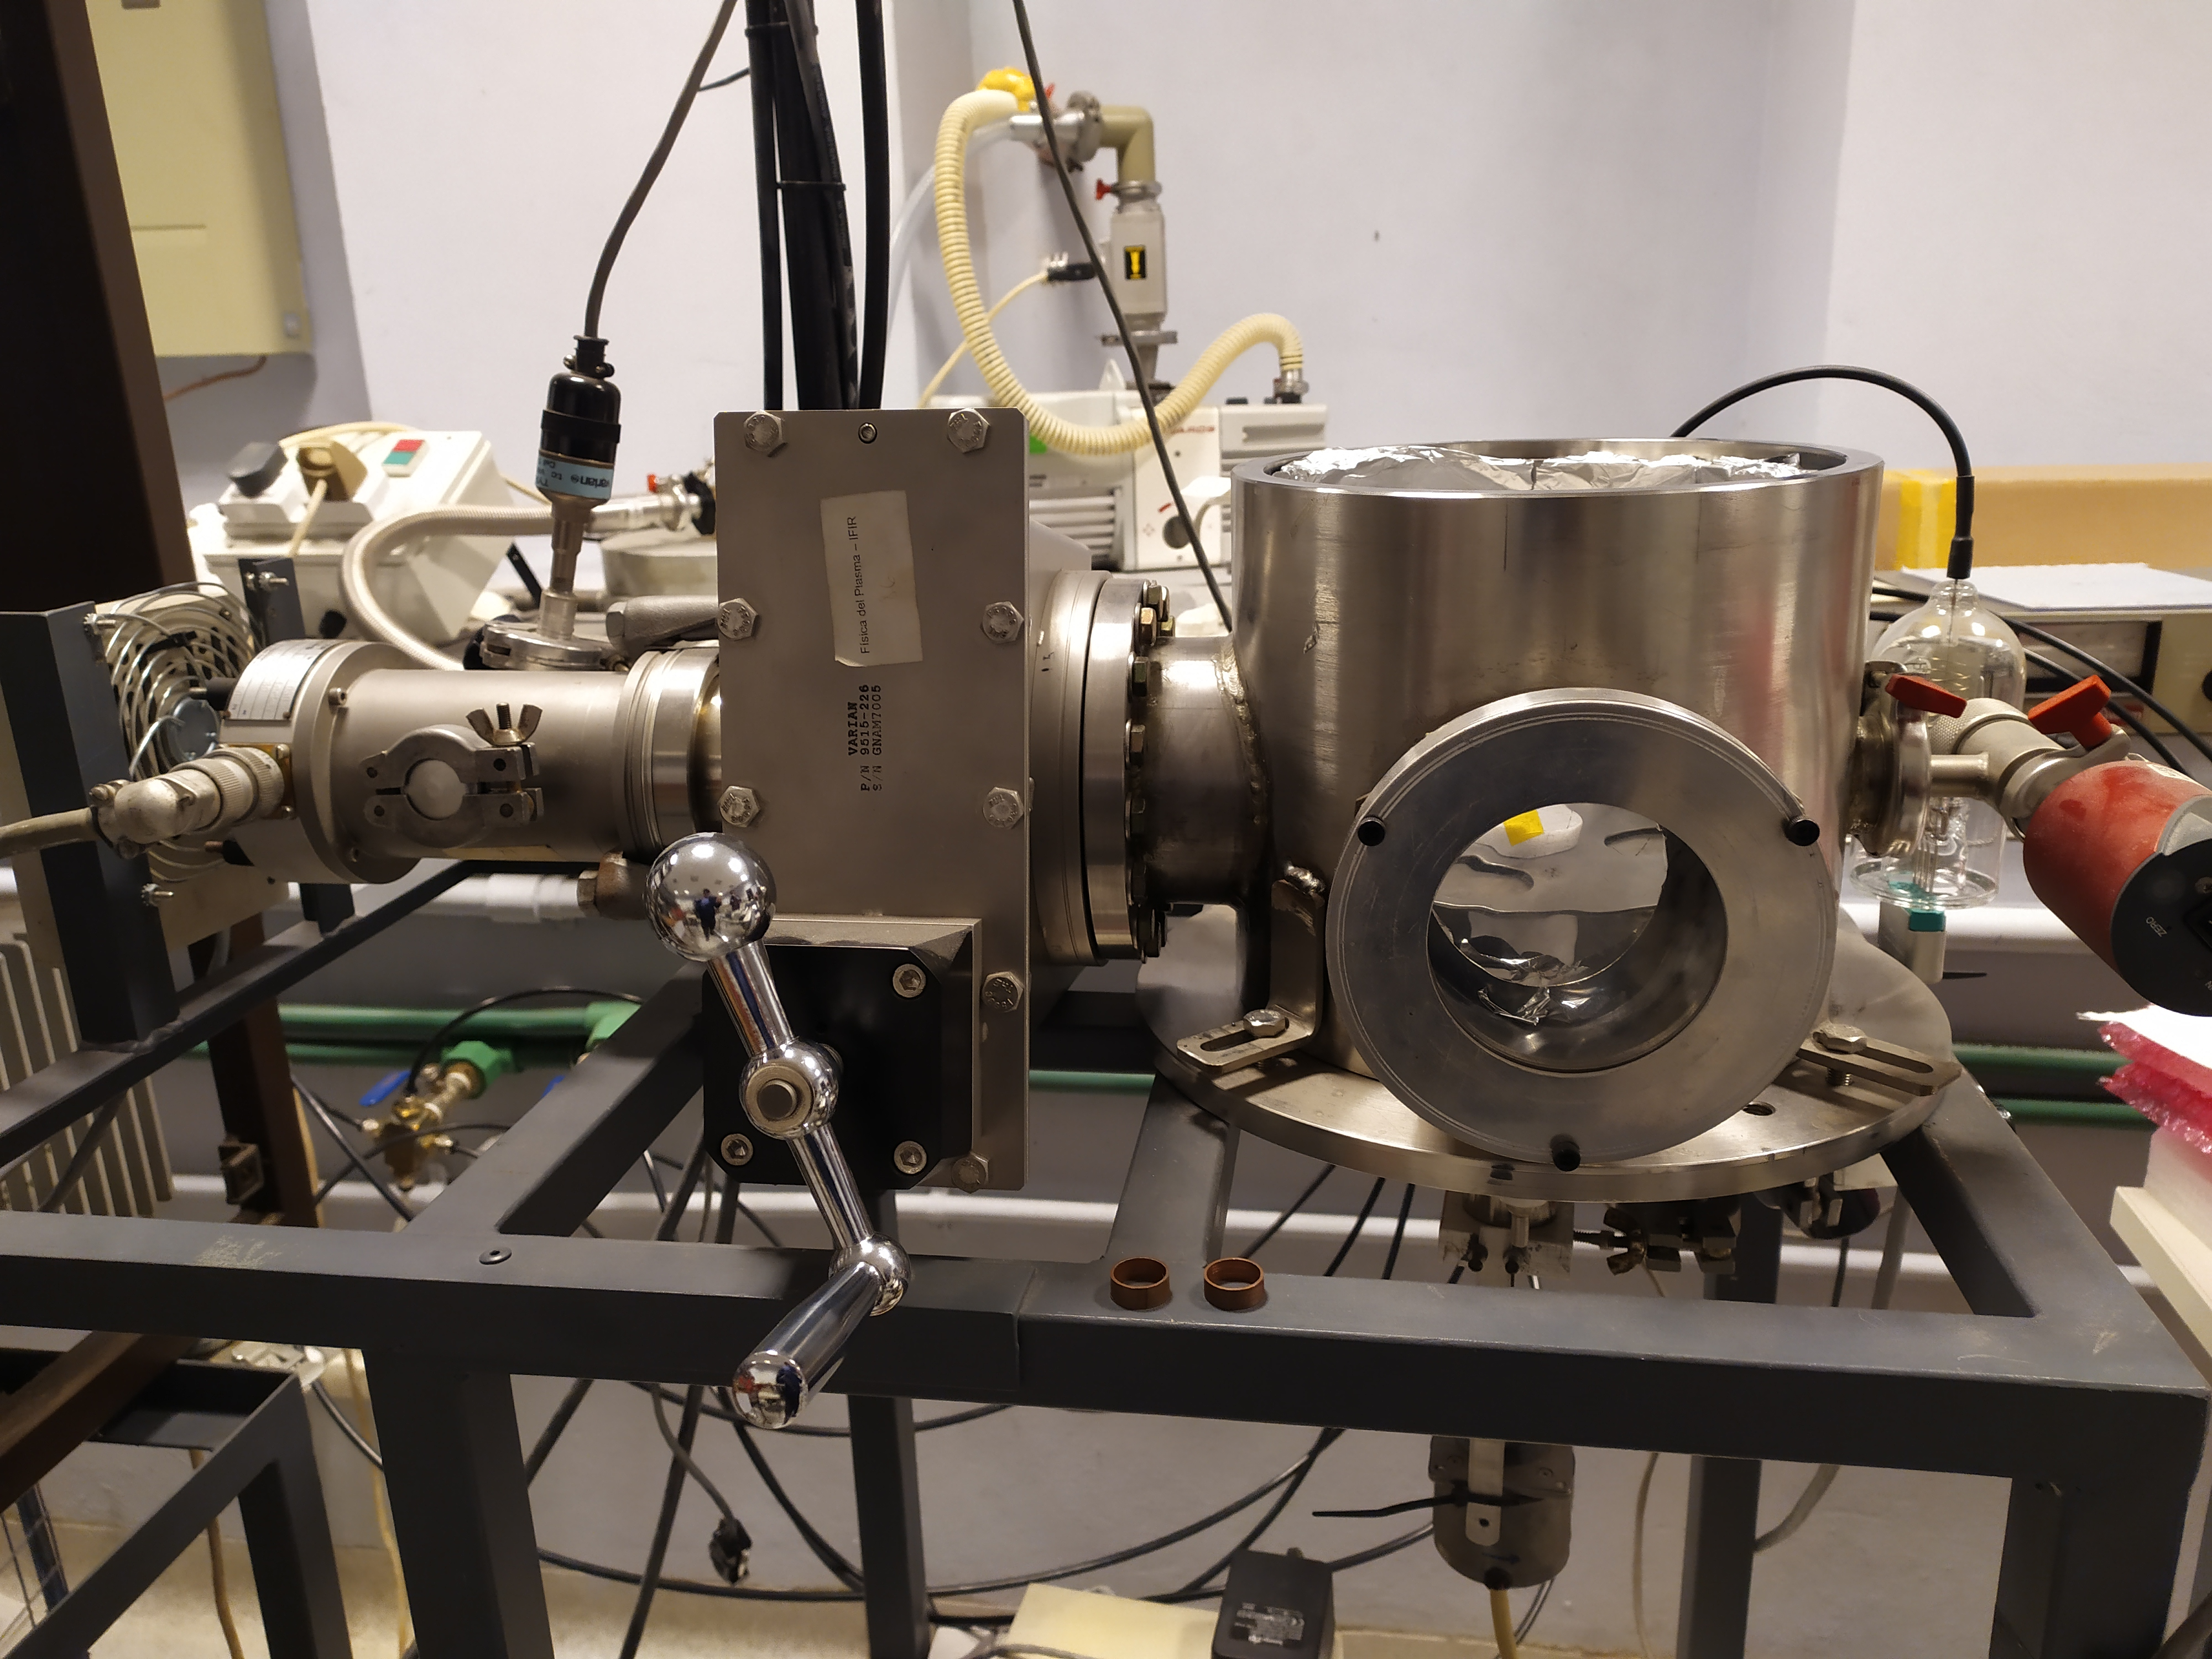
\includegraphics[scale=0.1]{img/camara.jpg}
	\caption{Cámara empleada para realizar las deposiciones.}
	\label{camara}
\end{figure}

\subsubsection{Sistema de vacío}

Durante realizar la deposición de los materiales se utilizó una atmósfera de $3 mTorr$ de argón dentro de la cámara. Se eligió $Ar$ como gas ya que al ser inerte no hay posibilidad que reaccione con alguno de los metales a ser depositados.


Para llegar al nivel de vacío requerido, se usó una bomba turbomolecular Varian V70S que alcanza un vacío base de $1,5 \times 10^{-6}Torr$. Esta bomba requiere un vacío previo, para lo cual se utilizó una bomba mecánica de dos etapas Edward Rv8 capaz de reducir la presión hasta $10^{-3}Torr$. La medición de vacío se realizó con un medidor de presión capacitivo Pfeiffer CMR 365 para el rango de trabajo ($\sim10^{-3}Torr$) y un Bayard-Alpert (cátodo caliente) Varian para la medición de vacío base ($10^{-4}Torr$ a $10^{-9}Torr$).

Para reducir el caudal durante la deposición y no dañar el sistema de vacío, se utilizó una válvula plato, colocada entre la bomba turbomolecular y la cámara de deposición, cerrada parcialmente.


\subsubsection{Sistema eléctrico}

El sistema eléctrico usado para alimentar los magnetrones era idéntico e independiente para cada uno de los magnetrones. Estos sistemas estaban compuestos de la siguiente manera: Un transformador Variac a 220$V$; Un transformador que permitía elevar la tensión hasta 1000$V$; Un puente rectificador; y dos multímetros conectados en conexión corta para medir la tensión y la corriente.

Al buscarse trabajar con potencia constante y no poder evitar variaciones en la tensión de entrada, se realizaban manualmente ajustes en el primer transformador Variac para regular la tensión de entrada y mantenerla lo más cercana posible a un valor constante.

\subsubsection{Colocación de los sustratos}

El sistema de soporte de los sustratos fue construido utilizando dos platos de acero inoxidable, colocados uno sobre el otro, unidos por un eje construido en teflón. En el plato inferior se colocan los sustratos y el superior actúa como pantalla para evitar que se deposite material en los sustratos, hasta que las condiciones de descargas sean las adecuadas (presión y potencia estable). Al alcanzarse las condiciones deseadas, se hace girar únicamente el plato superior lo suficiente para que los sustratos queden expuestos. Durante la deposición se hace girar todo el sistema en forma conjunta, a una velocidad constante de 60 rpm, para que los sustratos se expongan a cada magnetrón y de esa manera se logren láminas uniformes. En la Figura \ref{muestras} se muestra una foto del sistema de soporte de los sustratos.

\begin{figure}[H]
	\centering
	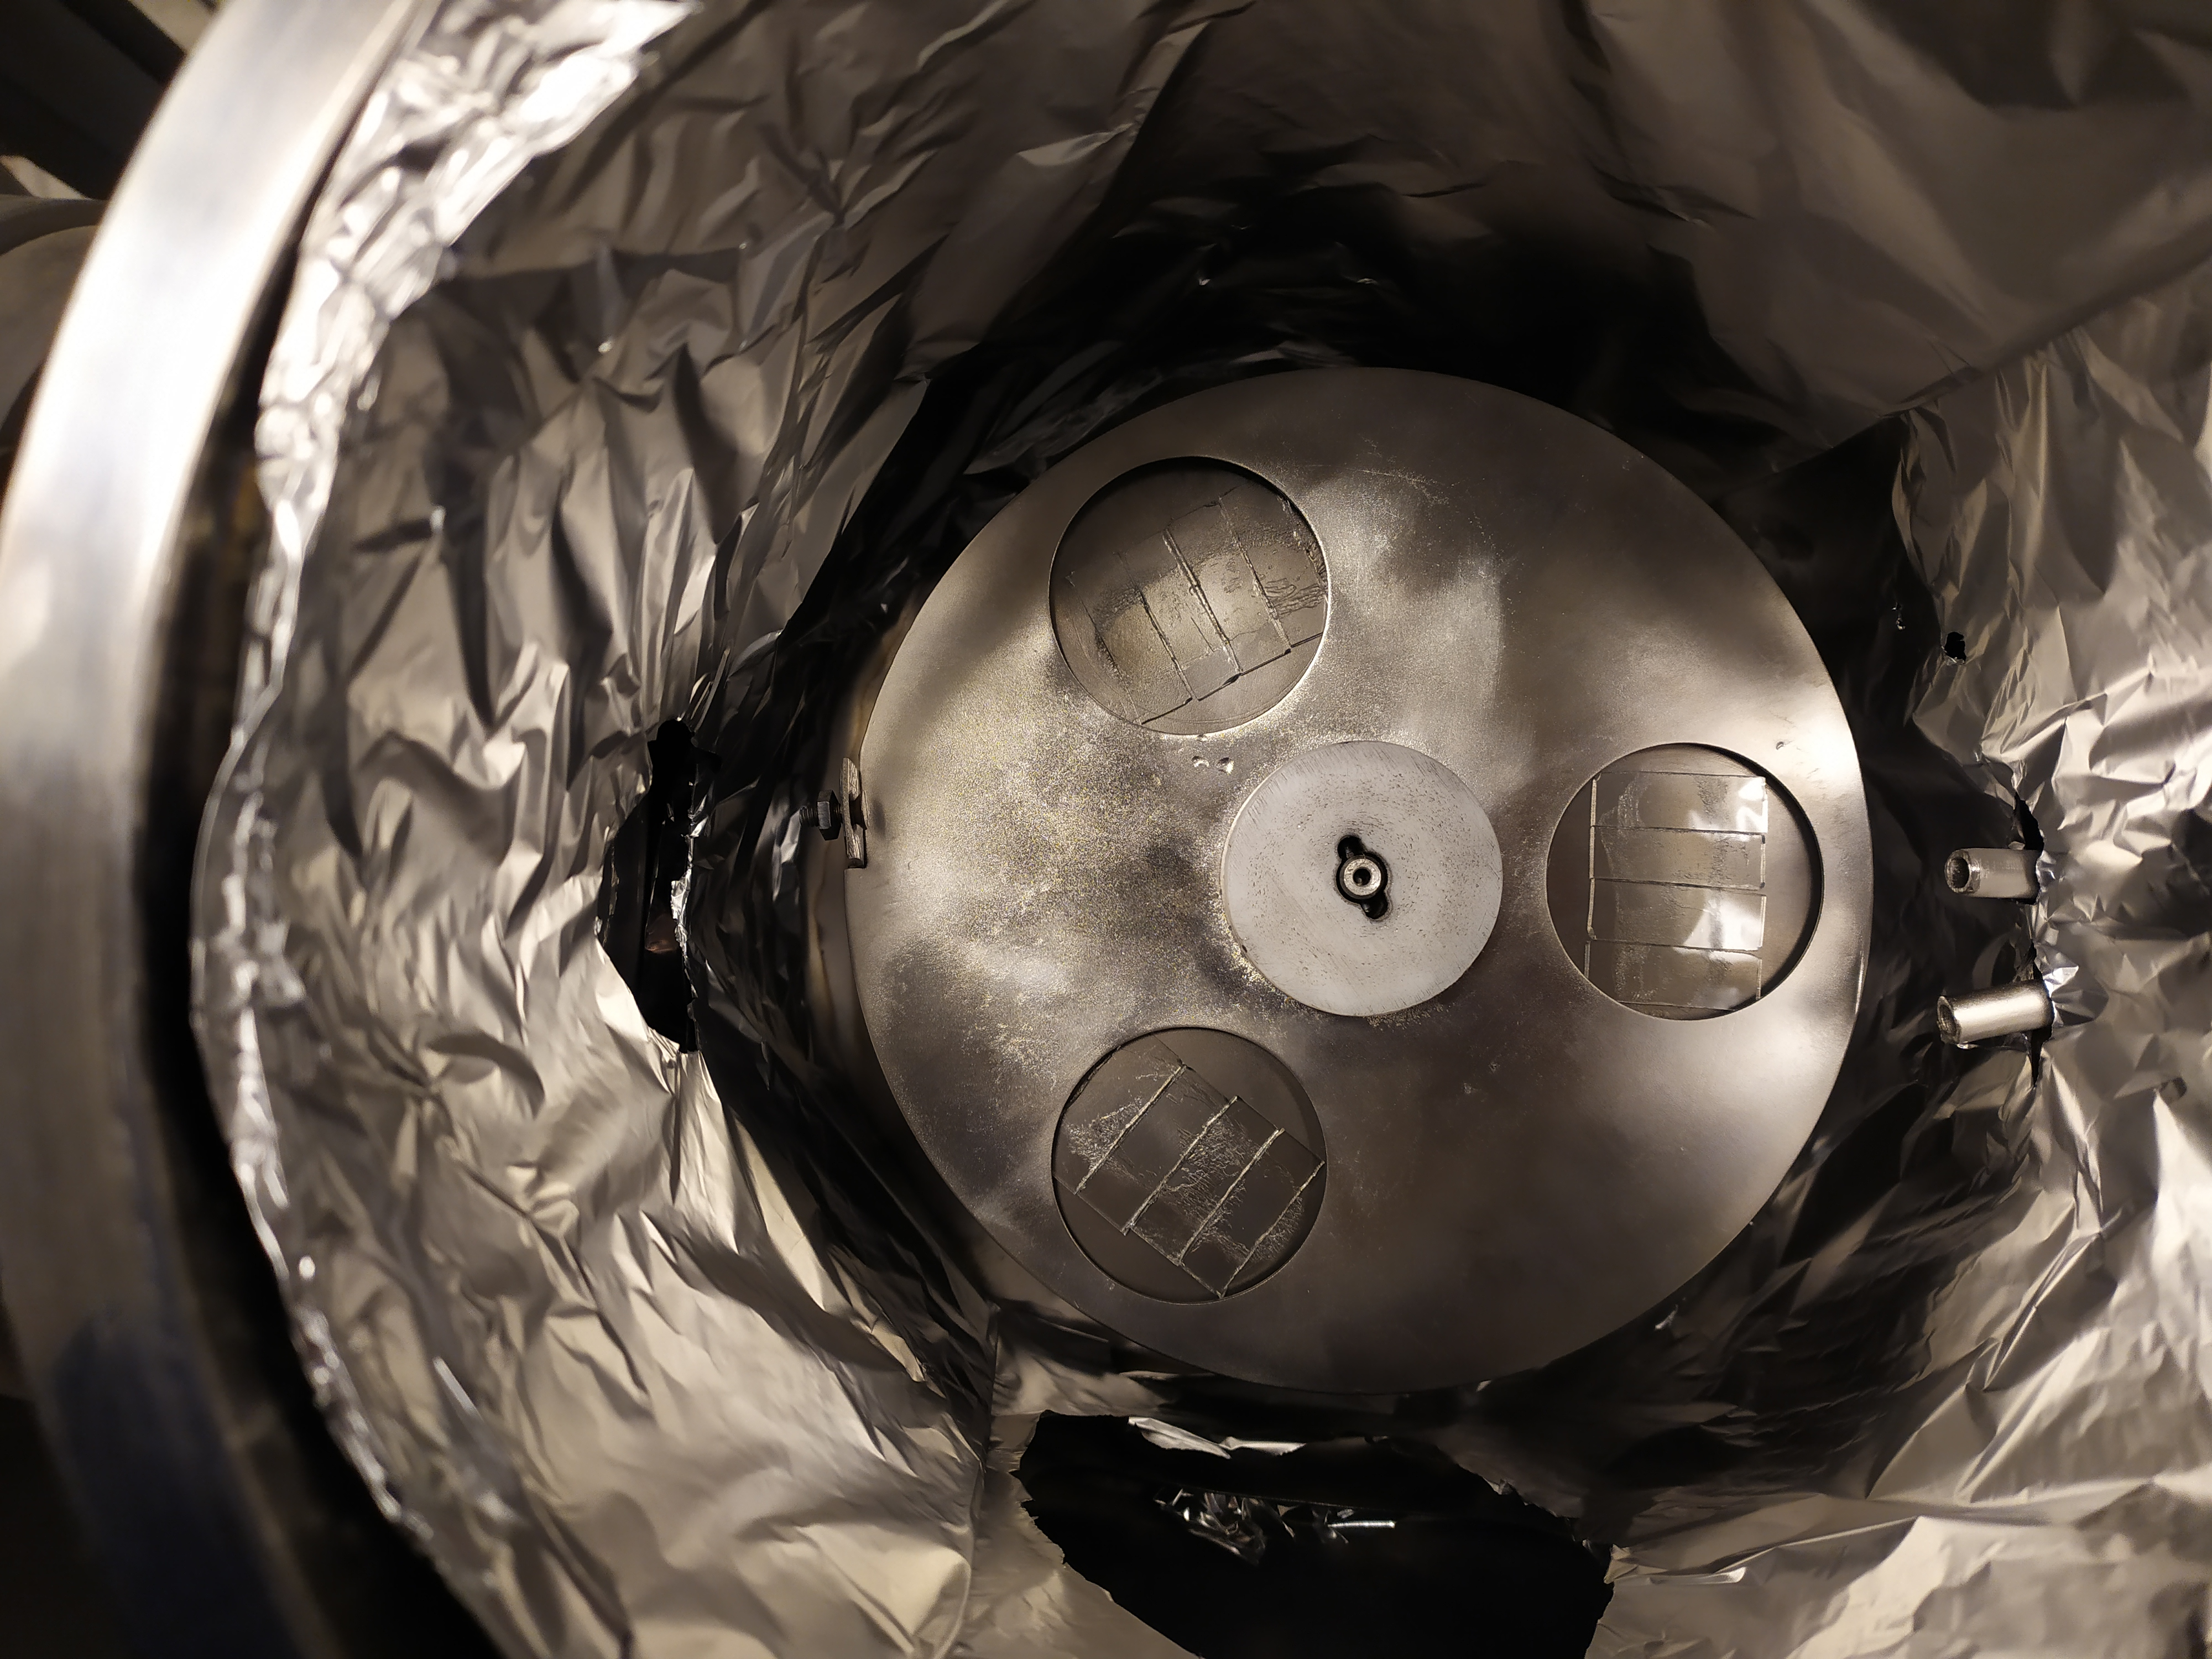
\includegraphics[scale=0.1]{img/muestras.jpg}
	\caption{Sustratos de vidrio colocados en el sistema de soporte rotatorio, antes de comenzar la deposición.}
	\label{muestras}
\end{figure}

\subsection{Microscopía electrónica de barrido}
El microscopio electrónico de barrido (\textbf{SEM}, del inglés \textbf{S}canning \textbf{E}lectron \textbf{M}icroscope) es un dispositivo que produce imágenes de alta resolución de la superficie de la muestra realizando un escaneo con un haz concentrado de electrones. Dichos electrones interactúan con la muestra produciendo varias señales que contienen información sobre la topografía de la superficie de la muestra y de su composición. Estas posibles señales son electrones secundarios, electrones retrodispersados, rayos X característicos, corriente absorbida y electrones transmitidos, siendo las operatorias más comunes la de electrones secundarios y la de rayos X.

Los electrones secundarios son emitidos por los átomos que ocupan la superficie superior y producen una imagen fácilmente interpretable de la superficie. El contraste de la imagen está determinado por la morfología de la muestra y la resolución de la misma depende del diámetro del haz de electrones primario. Este, en general, es del orden de los nanómetros, controlado por el tipo de generador de los electrones (termoiónicos, vía transistores de efecto de campo (FET), etc.) y la ''óptica” asociada.

La interacción del haz primario con los átomos de la muestra genera transiciones de los electrones entre distintos niveles de energía que dan lugar a la emisión de rayos X que tienen la energía característica del elemento emisor. La detección y medición de la estas energías permite realizar un análisis elemental, ya que cada átomo tiene su patrón de emisión característico. Este análisis se denomina espectroscopía EDS.

Como fuente de electrones estos dispositivos tienen distintos tipos de cañones para generar haces de alta o baja energía. En el caso de muestras metálicas, al no haber riesgo de dañar la muestra se usan haces de alta energía para conseguir la mejor resolución posible. Los electrones emitidos pasan a través de una columna en vacío donde el haz inicial es concentrado por lentes electromagnéticas llamadas lentes condensadoras y lente objetivo, con el propósito de obtener una mejor resolución en la imagen final. Luego, el haz es direccionado sobre toda la superficie mediante una serie de bobinas deflectoras para generar las interacciones de los electrones con el material y producir las señales antes descriptas. Finalmente, estas señales son captadas por los detectores adosados al equipo.

 \begin{figure}[H]
 	\centering
	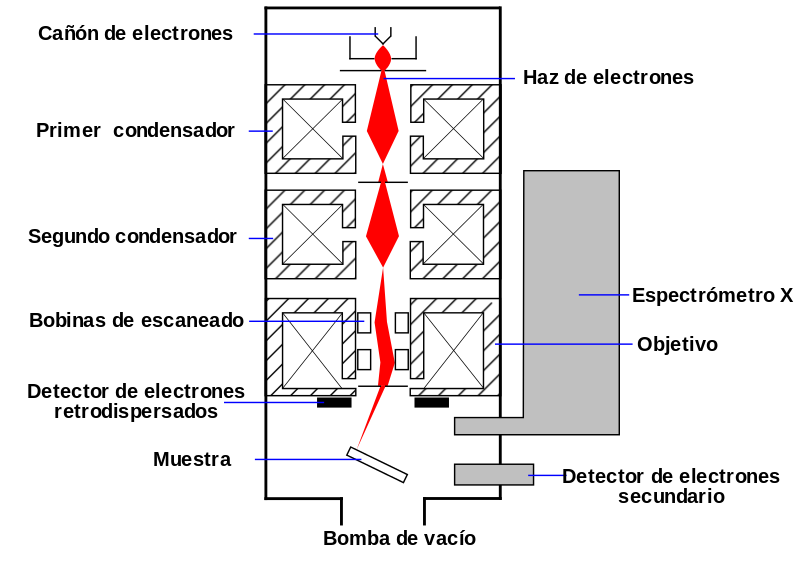
\includegraphics[scale=0.5]{img/SEM.png}
 	\caption{Esquema del tubo de un microscopio electrónico de barrido.}
	\label{SEM}
\end{figure} 

Para analizar la composición química de las láminas delgadas se utilizó un SEM Leitz Wetzlar AMR1000 con filamento de tungsteno, el cual tiene un detector de rayos X SDD (Silicon Drift Detector) modelo Oxford X-MAX. Los datos fueron analizados con el software AZtec 3.0.

El análisis de composición se realizó utilizando patrones de metales de $Ni$ y $Ti$ (ambos pureza $99,99$ \%), mientras que para el $Zr$ se utilizó el patrón de fabrica del detector. Además, antes de cada medición, se midió la intensidad del pico de rayos X sobre una muestra de $Co$ puro, con el objetivo de estandarizar la corriente del filamento estuviese estabilizada. De esta manera, las mediciones son hechas con la misma corriente y pueden ser comparables y reproducibles.

\subsection{Difracción por rayos X}
 La difracción por rayos X es una técnica para determinar la estructura cristalina de un material. Al recibir la muestra un haz incidente de rayos X, los electrones lo absorben para luego vibrar a dicha frecuencia como un dipolo, emitiendo así radiación de la misma frecuencia a la incidente. En este proceso se producen fenómenos de difracción e interferencia.  Conociendo las intensidades y los ángulos de dichos haces difractados es posible determinar la estructura del material.
 
\begin{figure}[H]
\centering
\subfloat[Reflexión de Bragg en planos atómicos.]{
  
\includegraphics[width=70mm]{img/Bragg.png}
} \\
\subfloat[Esquema del dispositivo tipo Bragg-Brentano.]{
  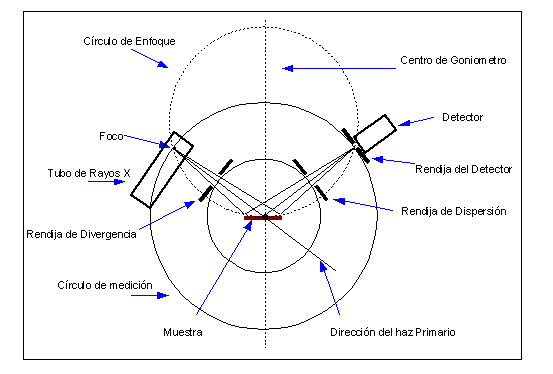
\includegraphics[width=70mm]{img/gonio.png}
}
\caption{Esquemas explicando el funcionamiento de un dispositivo tipo Bragg-Brentano.}
\label{Rxesquema}
\end{figure}
 
 Este fenómeno de difracción sucede cuando la longitud de onda de la radiación incidente es comparable a las distancias entre los átomos del material. Esta distancia es del orden de 0,15 a 0,4 $nm$, que en el espectro electromagnético corresponde a los rayos X, con energías entre 3 y 8 $keV$. En el caso que se emplease una longitud de onda mayor, rayos UV por ejemplo, se obtendría menor resolución y si se usase una longitud de onda menor, se correría el riesgo de alterar la muestra debido a la alta energía que poseería la radiación.
 
 
 Este fenómeno de difracción puede ser explicado mediante la Ley de Bragg. La radiación electromagnética incide en los diferentes planos atómicos, la cual al ser re-emitida presentará un fenómeno de interferencia debido a una diferencia de recorrido. La interferencia será constructiva en caso de que la distancia entre los planos cumpla con:
 
{\begin{equation}
 2 \, d\, {\rm sin} \theta =n \, \lambda \, \,; \, \, n \in \mathbf{N}
 \end{equation}
 
  \noindent donde $d$ es la distancia entre los planos cristalinos, $\theta$ el ángulo de difracción, $\lambda$ la longitud de onda y $n$ un número natural (ver Figura \ref{Rxesquema}).
 
 Entonces, la intensidad del haz difractado es medida para diversos ángulos, en este caso de $10^{\circ}$ a $120^{\circ}$ y es mostrada en función del parámetro $2\theta$. Al deberse este patrón de intensidades  a factores principalmente geométricos de la estructura, se emplea para discernir distintas estructuras y encontrar valores característicos como la distancia entre planos o los parámetros de red de la celda unidad.

 El dispositivo usado para las medición presentado en este trabajo fue un difractómetro de rayos X PANalytical-Empyrean en la configuración $\theta - 2\theta$.
 
\subsection{Microscopía electrónica de transmisión}
La microscopía electrónica de transmisión, conocida normalmente como \textbf{TEM} (del inglés, \textbf{T}ransmission \textbf{E}lectron \textbf{M}icroscopy) es una técnica de microscopía en la cual un haz de electrones atraviesa una muestra para formar una imagen. El poder de resolución de esta técnica se sitúa en el orden de $1 \AA$, resolución lograda ya que la longitud de onda de de Broglie de electrones muy energéticos es considerablemente menor que aquella de la luz visible (un microscopio óptico permite como máximo una resolución de aproximadamente 300 $nm$). Para realizar esta técnica se requiere que la muestra tenga un grosor menor a $100 nm$, debido al escaso poder de penetración de los electrones.

Al igual que en un microscopio electrónico de barrido, un microscopio electrónico de transmisión consiste de un cañón de electrones y de un conjunto de lentes magnéticas dentro de una columna de vacío. El esquema en particular para este útlimo se muestra en la Figura \ref{TEM}. La disposición de las lentes magnéticas para controlar el haz es similar a la disposición de lentes ópticas en un microscopio óptico.

 \begin{figure}[H]
 	\centering
	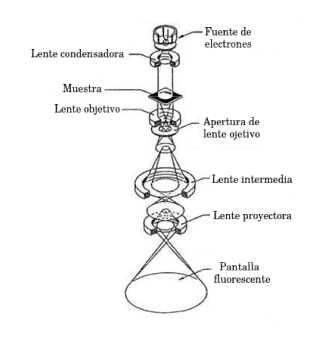
\includegraphics[scale=0.9]{img/TEM.png}
 	\caption{Esquema del tubo de un microscopio electrónico de transmisión.}
	\label{TEM}
\end{figure} 

Una lente magnética es un dispositivo que permite el foco o la deflección de partículas con carga usando la fuerza de Lorentz. Normalmente formadas por bobinas por las cuales circula corriente rodeadas por materiales ferromagnéticos diseñados para concentrar el campo magnético en un espacio confinado. La distancia focal de estas lentes es regulado variando la corriente que circula por las bobinas.

La lente condensadora permite producir un haz de electrones colimado incidente sobre la muestra. Luego de atravesar la muestra, el haz de electrones pasa por una lente objetivo, cuya tarea es formar una imagen magnificada hasta 40 veces en el plano focal de la siguiente lente, la lente intermedia. Esta lente produce una magnificación aún mayor que llega a la lente proyectora. Esta última lente reproduce la imagen, una vez más aumentada, sobre el receptor final de imagen, normalmente una pantalla fluorescente.

Ajustando las lentes electromagnéticas es posible generar un espectro de difracción en lugar de recrear la imagen. Este patrón consiste en diversos puntos en el caso de un cristal simple, una serie de anillos en el caso de una muestra policristalina, o discos difusos en el caso de un sólido amorfo. Como el patrón de difracción depende de la estructura de la muestra y de sus distancias interatómicos, con este patrón es posible conocer dichas propiedades. En caso de tener un sólido con múltiples fases, se colima el haz de electrones para que incida únicamente sobre una región deseada, y se obtiene el patrón de difracción de esta área. Realizando el proceso sucesivas veces sobre los distintos granos, es posible obtener información sobre todas las fases presentes. Esto último es una gran ventaja en comparación con el estudio de rayos X, ya que con rayos X no es posible obtener los espectros por separado para cada fase.

El TEM empleado en el presente trabajo es uno modelo JEM210 Plus, marca JEOL. Para la emisión de electrones tiene un filamento de hexaboruro de lantano ($LaB_6$) y puede ser operado con un voltaje de hasta 200 $kV$.

\subsubsection{Preparación de las muestras}

Como se dijo anteriormente, para poder formar imágenes en TEM es necesario afinar las muestras hasta que su espesor sea menor a los 100 $nm$. Debido al espesor inicial de las láminas delgadas y su fragilidad, se optó por el método de adelgazamiento iónico. Este proceso consiste en acelerar iones de un determinado gas, en este caso y normalmente $Ar$, en un alto vacío en la dirección de la muestra. Este choque de iones va liberando átomos de la capa superior de la muestra, proceso que se mantiene hasta que se forma un pequeño orificio en la muestra y se consiguen zonas muy delgadas a su alrededor. En el caso de muestras cristalinas, se produce la amorfización de las capas cercanas a la superficie (unos pocos nanómetros). Sin embargo, la estructura cristalina original permanece dentro de la muestra y las capas amorfas no interfieren con la observación. 

El equipo empleado para este tratamiento fue un afinador iónico Gatan PIPS 691.
 

\subsection{Tratamientos térmicos}

Para que las láminas obtenidas presenten una estructura cristalina es necesario realizarles un tratamiento térmico. Para llevar a cabo este procedimiento, se empleó un horno tubular con un controlador de temperatura para mantener la temperatura constante. Para mayor precisión en la medición de la temperatura, se empleó una termocupla envainada tipo K al lado de la muestra. 

Cada lámina fue envuelta dentro de una hoja de tantalio y luego encapsulada.
Las cápsulas empleadas fueron de vidrio para aquellas muestras tratadas hasta $600 ^\circ C$, y en cuarzo para las cápsulas tratadas a mayor temperatura. Dentro de las cápsulas, la atmósfera era de $Ar$ a 3 $mTorr$. Para generar esta atmósfera, primero se generó un vacío base dentro de la cámara de 0,3 $mTorr$. Hecho esto, se realizaron tres lavados llenando la cámara hasta presión atmosférica con $Ar$ y luego generando vacío hasta el vacío base nuevamente. Finalizado este proceso, las cámaras eran selladas con una presión interna de 3 $mTorr$.

El propósito de estos lavados y de la atmósfera era evitar que quedase oxígeno que pudiese oxidar las muestras. Así mismo, el tantalio se eligió porque resiste las temperaturas aquí empleadas (hasta 800 $^\circ C$) y para que tome el residuo de oxígeno dentro de las cápsulas, oxidándose así en lugar de las muestras.

\subsection{Calorimetría diferencial de barrido}

La calorimetría diferencial de barrido, llamada normalmente DSC (del inglés, differential scanning calorimetry) es una técnica termoanalítica en la cual se mide la diferencia de calor requerida para calentar una muestra y una referencia como función de la temperatura. La medición suele realizarse en una atmósfera controlada de un gas inerte, y con rampas programadas de cambio de temperatura en función del tiempo.  Es necesario destacar que la referencia debe ser inerte en el rango de temperaturas medido.
Esta técnica permite determinar las temperaturas a las cuales ocurren distintos procesos en los materiales, como transformaciones de fase o reacciones químicas. Además, es posible determinar el calor específico y el cambio de entalpía que acompañan las transiciones de primer y segundo orden, ya sean procesos exotérmicos o endotérmicos.

El calorímetro usado fue el modelo Shimadzu DSC-60, cuyo esquema se muestra en la Figura \ref{DSCscheme}. Para usarlo, se configura un programa que controla la temperatura del bloque calefactor ($T_b$), del cual fluye calor a través de una resistencia R hacia la muestra y la referencia, haciendo que la temperatura de la muestra ($T_m$) y la temperatura de la referencia ($T_r$) cambien al igual que $T_b$. La diferencia entre la $T_m$ y $T_r$ es $\Delta T = T_m - T_r$. Cuando una muestra se funde, su temperatura se mantiene constante mientras que la temperatura de la referencia sigue aumentando. Cuando esto sucede, es necesario entregarle mucho más calor a la muestra para que su temperatura se mantenga igual a la de la referencia. En caso de una solidificación, lo inverso ocurre.

\begin{figure}[h]
	\centering
	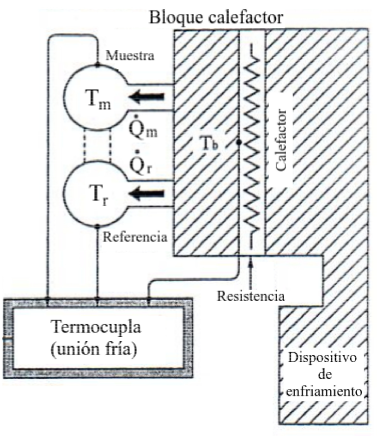
\includegraphics[scale=0.5]{img/DSCscheme.png}
	\caption{Esquema del DSC empleado.}
	\label{DSCscheme}
\end{figure}

El área debajo de los picos registrados es proporcional a la energía calórica necesaria para la transformación o reacción que sucede. En condiciones de presión constante, la energía calórica es igual al cambio de entalpía $\Delta H$ de la muestra.

En el trabajo se utilizaron panes de aluminio de 5 mm de diámetro, dentro de los cuales se colocaron múltiples trozos de las láminas delgadas hasta alcanzar una masa cercana a los 5 mg.


\subsection{Resistividad por el método de cuatro puntas}

Al cambiar un material su estructura atómica, lo normal es que muchas de sus propiedades se vean afectadas, entre ellas la resistividad. Si esta transformación sucede mientras circula una corriente eléctrica a través del material, se observará un cambio en la resistencia del material asociado a la transformación de fase. De esta manera, si se le aplica una corriente constante al material, midiendo la diferencia de potencial es posible determinar donde comienzan y terminan los cambios de fase.


La medición de resistividad por cuatro punta consiste en aplicar una corriente constante $I$ a través de dos contactos y medir  la caída de potencial $\delta V$ con otros dos contactos en la zona de circulación de la corriente. De estos cuatro contactos deriva el nombre del método. Un esquema de la disposición se muestra en la Figura \ref{4puntas}. La lámina es sujetada en una base de cobre, llamada dedo frío, mediante los cuatro contactos fabricados con alambre de Constatán, soldados a cuatro chapas elásticas de acero para asegurar un buen contacto eléctrico.

 \begin{figure}[H]
 	\centering
	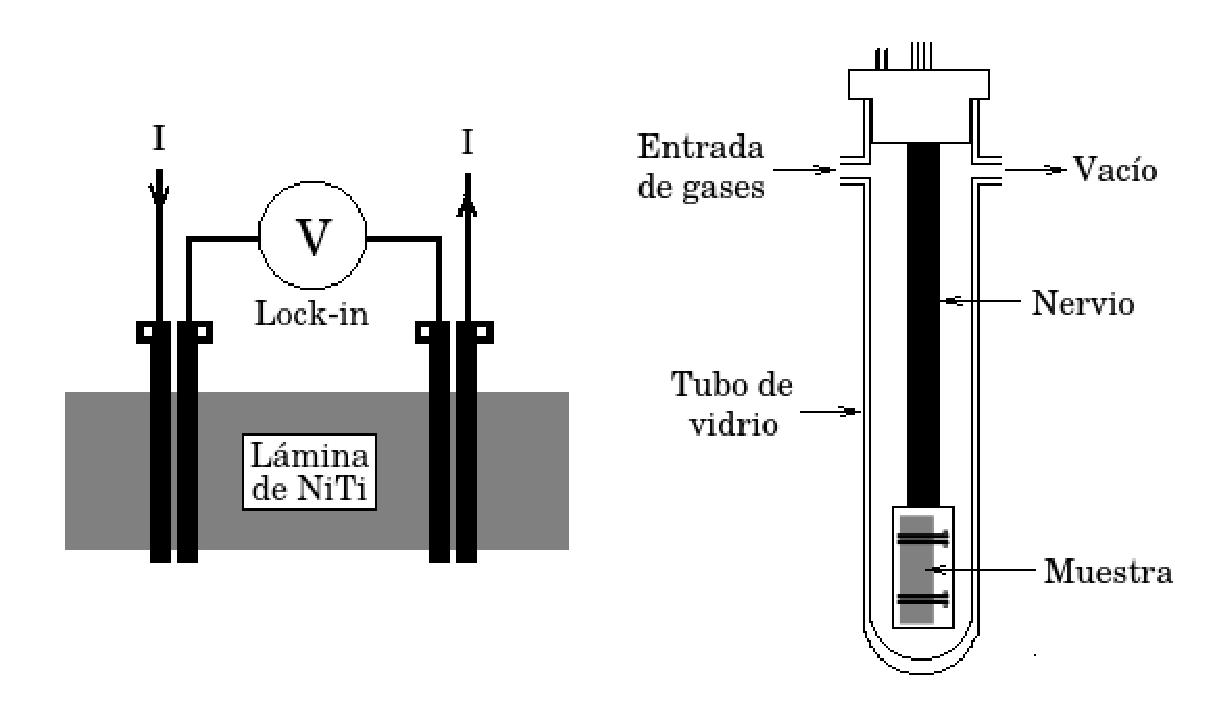
\includegraphics[scale=0.7]{img/resistividad.eps}
 	\caption{Esquema de el sistema empleado para el método de resistividad por cuatro puntas.}
	\label{4puntas}
\end{figure} 

Toda esta estructura se encuentra dentro de un tubo de vidrio cerrado, lo cual permite que el sistema sea sumergido en nitrógeno líquido para trabajar con la muestra a bajas temperaturas. Por arriba, el tubo está cerrado con un tapón de teflón. Este tapón cuenta con un o'ring que garantiza el cierre hermético con las paredes del tubo y, además, por cada contacto eléctrico también hay un pequeño o'ring. Los contactos son ajustados por una única tapa superior ajustada por tres tornillos. Los cables que pasan a través del tapón son los siguientes:
\begin{itemize}
\item Dos contactos por los cuales circula la corriente.
\item Dos contactos para medir la diferencia de potencial.
\item Un contacto para la termocupla de medición.
\item Un contacto a tierra dentro del tubo.
\item Dos contactos para conexión del controlador de temperatura.
\item Dos contactos para la termocupla del controlador de temperatura.
\end{itemize}


Dentro del dedo frío hay una resistencia eléctrica alimentada desde el controlador de temperatura Novus 1200, calentando la muestra por efecto Joule y dos termocuplas tipo K. Una de ellas se utiliza para el controlador de temperatura, mientras que la otra termocupla mide la temperatura de la muestra a través de una punta fría y un multímetro Agilent 34401a. Al estar la muestra cubierta con lana de alúmina, esta intercambia calor únicamente con el dedo frío, por lo cual puede considerarse que tanto muestra como dedo frío están siempre a la misma temperatura.

En la parte superior del tubo hay dos aberturas laterales. Una de ellas está conectada a un acople T que conecta un tubo de $Ar$ y otro de $He$. La otra abertura se conecta con una bomba de vacío.

Al ser la muestra un material conductor, la diferencia de potencial medida es muy pequeña (orden de los $\mu V$), por lo cual el instrumento para llevar a cabo la medición debe ser de alta precisión y con filtros de ruido. El equipo usado para esta tarea fue un amplificador Lock-in modelo Sr-510 Stanford Research. En los contactos exteriores se aplicó una corriente de aproximadamente $10mA$, generada con un generador de señal operando a un 1 $kHz$ a través de una resistencia de 1$k\Omega$. El amplificador Lock-in y el multímetro Agilent se conectan a un sistema de adquisición de datos en una computadora. 

Todas las mediciones se realizaron en una atmósfera de He a 660 $Torr$ y un vacío base de 20 $mTorr$. Se trabajó en una atmósfera inerte para evitar que la condensación de la humedad ambiente a bajas temperaturas afectase la medición, y se eligió atmósfera de $He$ en lugar de $Ar$ ya que el último se condensa dentro del rango de temperaturas en el cual se trabajó (desde $\sim 120 ^\circ C$ hasta $-140 ^\circ C$). La velocidad de enfriamiento y calentamiento se mantuvo a $\sim10^\circ C min^{-1}$.

\newpage
\section{Resultados obtenidos}

\subsection{Deposición de las láminas delgadas}

Las láminas  delgadas de $NiTiZr$ analizadas en esta Tesina fueron obtenidas en dos deposiciones distintas. En la Tabla \ref{potencias} se muestran los valores para la potencia promedio de cada magnetrón en ambas deposiciones. Los errores corresponden a las variaciones observadas durante las deposiciones, que fueron mayores a las incertezas de los instrumentos. Debido a las fluctuaciones de la tensión de línea y el desgaste de los blancos, fue necesaria la estabilización de la potencia de los magnetrones a través de los autotransformadores variables (Variac) y cada 10 minutos fue registrada la potencia de cada magnetrón.

En ambas deposiciones el vacío base alcanzado fue $3 \times 10^{-3}mTorr$ y la atmósfera de trabajo fue de $Ar$ a una presión de $3.0 \pm 0,1 mTorr$. Para que la deposición fuese uniforme, se hizo girar el sistema para sostener los sustratos a una velocidad de 60 rpm. Se obtuvieron 12 láminas de 8mm $\times$ 25mm aproximadamente en cada una de las deposiciones.

\begin{table}[H]
\centering
\begin{tabular}{|c|c|c|}
\hline
 & Primera deposición  & Segunda Deposición \\ \hline
$P_{Ti}[W]$ & $200 \pm 5$ & $200 \pm 5$ \\ \hline
$P_{Ni}[W]$ & $125 \pm 5$ & $117 \pm 5$ \\ \hline
$P_{Zr}[W]$ & $90 \pm 5$ & $95 \pm 5$ \\ \hline
\end{tabular}
\caption{Potencia promedio empleada para cada uno de los blancos en las deposiciones.}
\label{potencias}
\end{table}

\subsubsection{Composición de las láminas}

De cada deposición se tomaron dos muestras y fueron analizadas con EDS-SEM para determinar su composición. En la Figura \ref{dep2} se muestra, a modo de ejemplo, uno de los espectros medidos para la primera deposición. Adicionalmente a $Ni$, $Ti$ y $Zr$ fueron detectados $Al$, $Si$, $O$, $C$ y $Fe$. La detección de $Al$ y $Fe$ es esperable, ya que el portamuestras es de aluminio y que el SEM cuenta con distintas piezas construidas con acero. El detector de EDS también está construido con $Si$, por lo cual también es esperable detectar este elemento. La medición de $O$ y $C$, al ser elementos livianos, no es confiable a través de \textcolor{violet}{esta técnica}. Por lo tanto, para el análisis cuantitativo de la composición de las láminas sólo se tuvieron en cuenta los elementos empleados en la aleación ($Ni$, $Ti$ y $Zr$).

 \begin{figure}[H]
 	\centering
	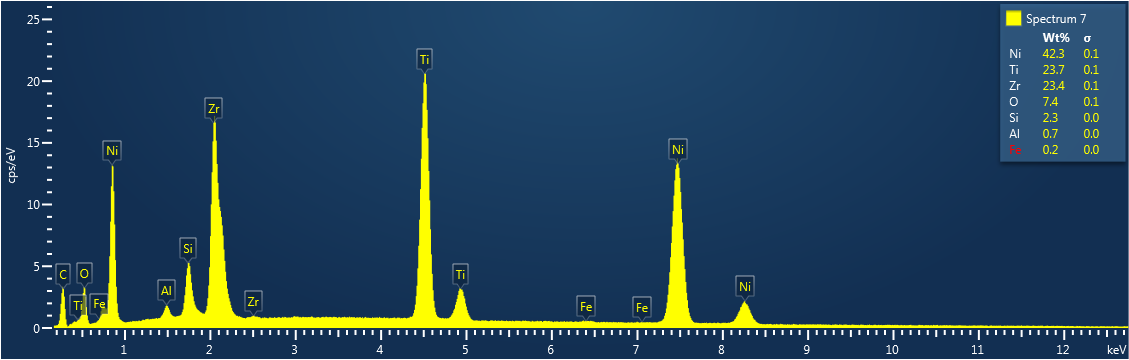
\includegraphics[scale=0.5]{img/SEMAllElements.png}
 	\caption{Espectrograma de la cara superior de una muestra de la segunda deposición.}
	\label{dep2}
\end{figure} 

Estas dos muestras se utilizaron para analizar la composición de la caras superiores e inferiores de las láminas, ya que la penetración de los electrones del SEM en este material es de aproximadamente 1 $\mu$m y el espesor de las láminas observadas en el SEM fue de 7 $\mu$m. Además, para estimar las variaciones locales de composición, se midió la composición de cada cara en tres regiones distintas, tomando una ventana de 40 $\mu$m $\times$ 40 $\mu$m en cada medición. En las Tablas \ref{composition2} y \ref{composition3} pueden verse las diferentes mediciones realizadas.


\begin{table}[H]
\begin{tabular}{c|c|c|c|c|c|c|}
\cline{2-7}
\multicolumn{1}{l|}{} & \multicolumn{3}{c|}{Cara superior} & \multicolumn{3}{c|}{Cara Inferior} \\ \cline{2-7} 
\multicolumn{1}{l|}{} & Región 1 & Región 2 & Región 3 & Región 1 & Región 2 & Región 3 \\ \hline
\multicolumn{1}{|c|}{Ti{[}\%at{]}} & 30,13 & 30,15 & 30,20 & 31,39 & 31,25 & 31,38 \\ \hline
\multicolumn{1}{|c|}{Ni{[}\%at{]}} & 50,56 & 50,56 & 50,53 & 50,23 & 50,27 & 50,22 \\ \hline
\multicolumn{1}{|c|}{Zr{[}\%at{]}} & 19,30 & 19,29 & 19,27 & 18,38 & 18,48 & 18,40 \\ \hline
\end{tabular}
\caption{Medición de composición para una muestra de la primera deposición en diferentes regiones.}
\label{composition2}
\end{table}

\begin{table}[H]
\begin{tabular}{c|c|c|c|c|c|c|}
\cline{2-7}
\multicolumn{1}{l|}{} & \multicolumn{3}{c|}{Cara superior} & \multicolumn{3}{c|}{Cara Inferior} \\ \cline{2-7} 
\multicolumn{1}{l|}{} & Región 1 & Región 2 & Región 3 & Región 1 & Región 2 & Región 3 \\ \hline
\multicolumn{1}{|c|}{Ti{[}\%at{]}} & 33,65 & 33,61 & 33,60 & 32,77 & 32,61 & 32,73 \\ \hline
\multicolumn{1}{|c|}{Ni{[}\%at{]}} & 44,86 & 44,85 & 44,91 & 47,05 & 47,20 & 47,28 \\ \hline
\multicolumn{1}{|c|}{Zr{[}\%at{]}} & 21,49 & 21,54 & 21,50 & 20,17 & 20,19 & 19,99 \\ \hline
\end{tabular}
\caption{Medición de composición para una muestra de la segunda deposición en diferentes regiones.}
\label{composition3}
\end{table}

En la Tabla \ref{compositionAvg} se ve el promedio de estas mediciones, y puede apreciarse que la primera deposición es rica en $Ni$, mientras que la segunda es pobre en $Ni$.


\begin{table}[H]
\centering
\begin{tabular}{c|c|c|}
\cline{2-3}
\multicolumn{1}{l|}{} & Primera Deposición 2 & Tercera Deposición \\ \hline
\multicolumn{1}{|c|}{Ti{[}\%at{]}} & 30,8 $\pm$ 0,6 & 33,2 $\pm$ 0,5 \\ \hline
\multicolumn{1}{|c|}{Ni{[}\%at{]}} & 50,4 $\pm$ 0,2 & 46 $\pm$ 1 \\ \hline
\multicolumn{1}{|c|}{Zr{[}\%at{]}} & 18,9 $\pm$ 0,5 & 20,8 $\pm$ 0,4 \\ \hline
\end{tabular}
\caption{Composición determinada para ambas deposiciones.}
\label{compositionAvg}
\end{table}

Las variaciones en la composición entre las diferentes caras de una misma lámina se explican por fluctuaciones en las condiciones de descarga de los magnetrones. 

\subsubsection{Difracción de rayos X}
Las láminas depositadas no presentaron estructura cristalina previo a los tratamientos térmicos. En la Figura \ref{amorfo} se muestra el difractograma de una muestra de la segunda deposición. La presencia del pico ancho cercano a los $2\theta=40^\circ$  es característico de una muestra amorfa. El pico de $Si$ se debe a que para la medición de rayos X se utilizó un portamuestras que contiene un wafer  de $Si$ monocristalino como base para la muestra.

\begin{figure}[H]
 	\centering
	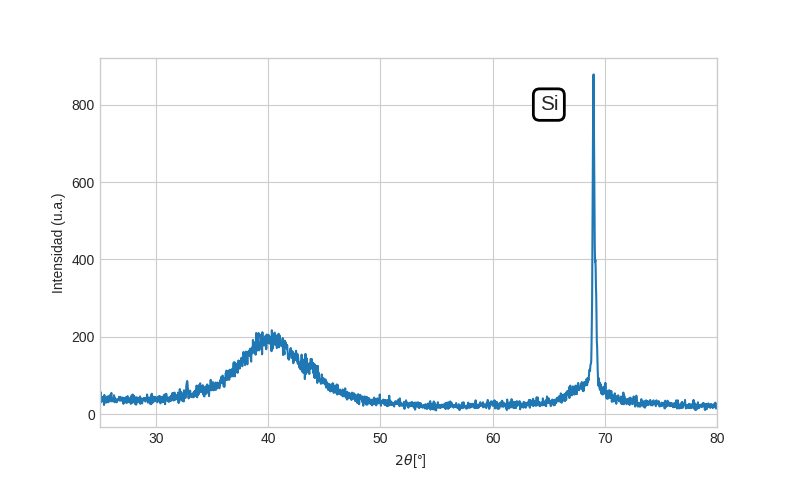
\includegraphics[scale=0.6]{img/RX_amorfo.png}
 	\caption{Difractograma de una muestra de la segunda deposición antes de realizar tratamientos térmicos.}
	\label{amorfo}
\end{figure}


\subsubsection{Temperaturas de cristalización y energía de activación}

Con el objetivo de analizar el proceso de cristalización de las láminas delgadas de $NiTiZr$, se realizaron calentamientos a distintas velocidades (5, 10, 20, 30 y 50 $^{\circ} C/min$) en las láminas obtenidas en la primera deposición. Para cada ensayo se empleó una lámina distinta, la cual se colocó dentro de un pan de aluminio. Dichas láminas tenían una masa de 6 mg cada una aproximadamente. En la Figura \ref{DSCPeaks} se muestran los picos exotérmicos observados en las mediciones y se indican las temperaturas donde el pico alcanza el máximo ($T_p$). Se supuso que la curva de base del DSC es lineal en el rango de temperatura donde se desarrolla el pico correspondiente a la cristalización.

\begin{figure}[H]
	\centering
	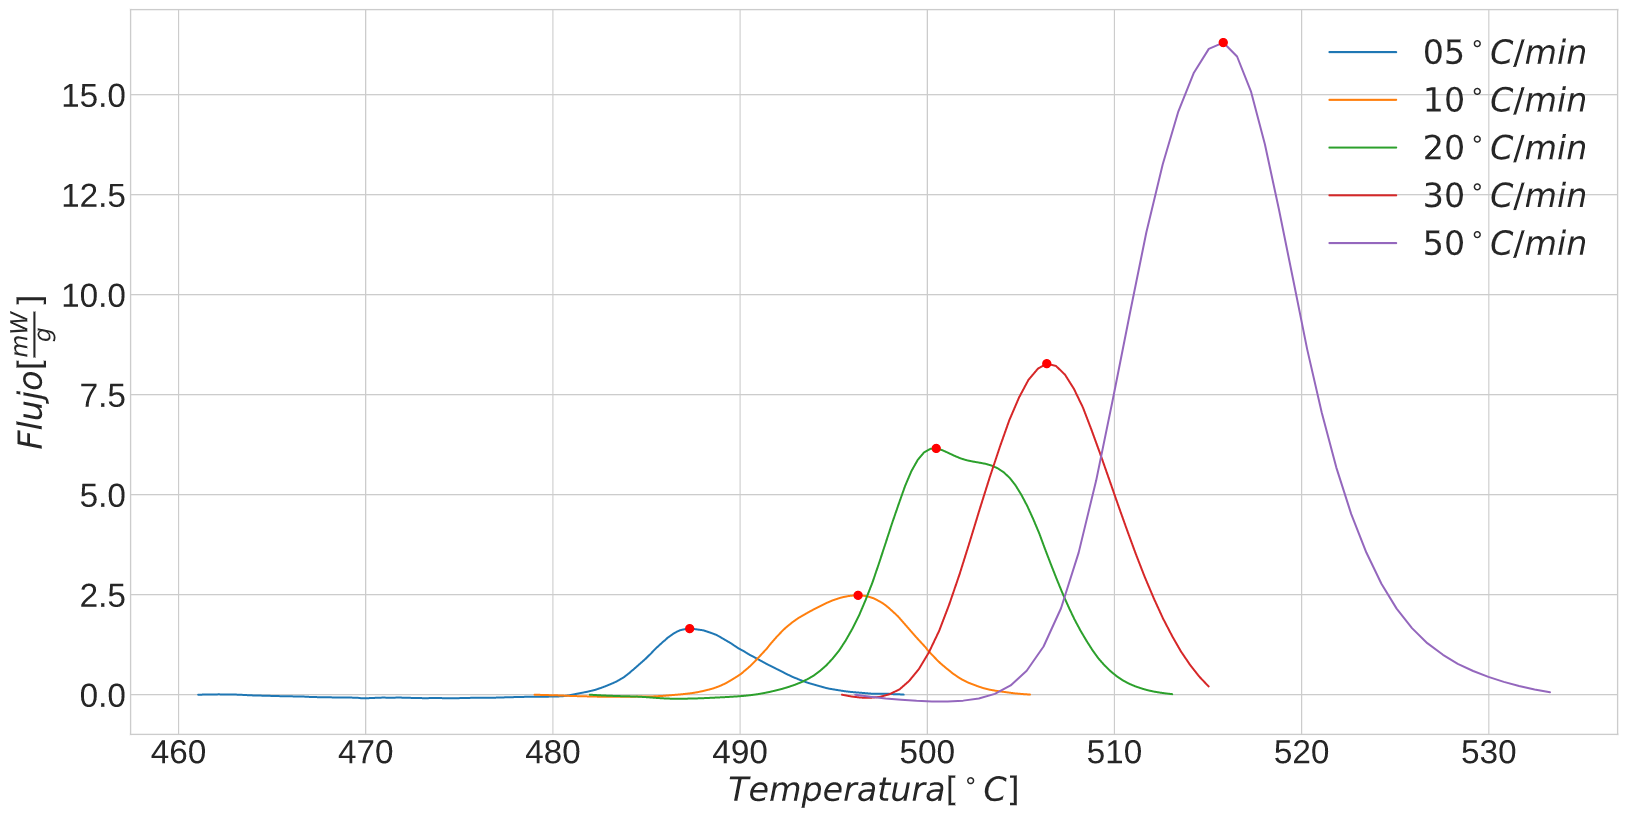
\includegraphics[scale=0.2]{img/DSCPeaks}
	\caption{Mediciones de los diferentes picos de DSC para distintas velocidades. El punto rojo indica la temperatura donde el pico alcanza su valor máximo ($T_p$).}
	\label{DSCPeaks}
\end{figure}

Debido a que el error relativo de $T_p^{-1}$ es mucho mayor que $ln(\frac{\alpha}{T_p^2})$ y que $ln(\frac{\alpha}{T_p-T_0})$, para poder realizar una regresión lineal se invirtieron los ejes, graficándose así $T_p^{-1}$ en función de $ln(\frac{\alpha}{T_p^2})$ y de $ln(\frac{\alpha}{T_p-T_0})$ para los modelos de Kissinger y Augis-Bennet respectivamente. Esto es:

\begin{equation}
\label{EquationKissinger}
	T_p^{-1}=-\frac{R}{E_c}ln(\frac{\alpha}{T_p^2})+cte
\end{equation}

\begin{equation}
\label{EquationAugisBennet}
	T_p^{-1}=-\frac{R}{E_c}ln(\frac{\alpha}{T_p-T_0})+cte
\end{equation}

Con un ajuste lineal realizado por mínimos cuadrados se obtuvo el valor de $E_c$ a través de la pendiente en cada modelo. Los puntos calculados usando las Ecuaciones \ref{EquationKissinger} y \ref{EquationAugisBennet} a partir de los medidos junto con los ajuste lineales se muestran en las Figuras \ref{Kiss} y \ref{AugBen}. A través del método de Kissinger el valor obtenido para la energía de activación fue de $(420 \pm 30) kJ$ mientras que por el método de Augis-Bennet el valor obtenido fue de $(410 \pm 30) kJ$.

\begin{figure}[H]
 	\centering
	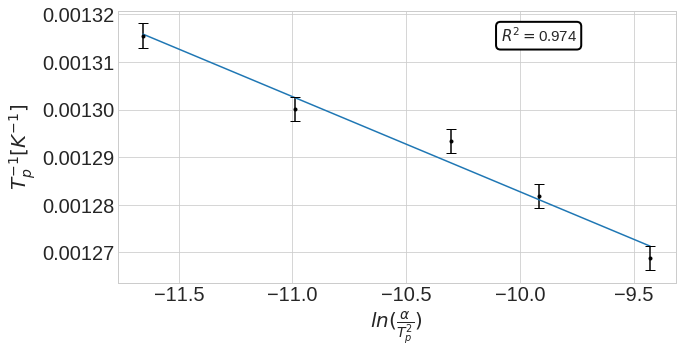
\includegraphics[scale=0.6]{img/Kissinger.png}
 	\caption{Regresión lineal realizada para la relación de Kissinger. Los valores obtenidos para el ajuste fueron: $m=(-2,0\pm0,1)\cdot10^{-5}; h=(-1,08\pm0,02)\cdot10^{-3}$.}
	\label{Kiss}
\end{figure} 

 \begin{figure}[H]
 	\centering
	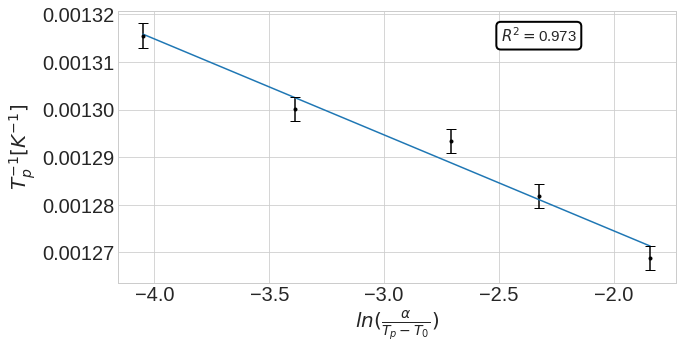
\includegraphics[scale=0.6]{img/Augis_bennet.png}
 	\caption{Regresión lineal realizada para la relación de Augis-Bennet.Los valores obtenidos para el ajuste fueron: $m=(-2,0\pm0,1)\cdot10^{-5}; h=(-1,234\pm0,004)\cdot10^{-3}$.}
	\label{AugBen}
\end{figure} 

\subsection{Tratamiento térmicos}

Para poder estudiar las microestructuras, fases presentes y su relación con la transformación martensítica, las láminas de ambas deposiciones fueron encapsuladas en vacío, con el objetivo de cristalizarlas mediante tratamientos térmicos a $500 ^\circ C$, $600 ^\circ C$, $700 ^\circ C$ y $800 ^\circ C$ durante $60$ min. Es importante notar que las láminas de la primera deposición tienen una composición rica en $Ni$, y, por el contrario, las láminas de la segunda deposición tienen una composición pobre en $Ni$. Esto permitió realizar un estudio completo del efecto de los tratamientos térmicos en la láminas de $NiTiZr$. Como contrapartida, algunas dificultades en el proceso de encapsulado produjeron algún grado de oxidación de las láminas en los tratamientos térmicos a mayor temperatura y, además, se observó que las láminas se presentaron frágiles luego de los tratamientos térmicos, por lo cual su manipulación posterior resultó muy dificultosa.

\subsection{Deposición pobre en $Ni$}
\subsubsection{Difracción de rayos X}
En la Figura \ref{RXNiPoor} se muestran los difractogramas de las láminas con composición pobre en $Ni$, luego de los distintos tratamientos térmicos. En dicha figura se muestra el logaritmo natural de la intensidad, de modo que todos los picos puedan ser apreciados. La identificación de las distintas fases se realizó a través de la simulación de las estructuras cristalinas con el programa PowderCell.

\begin{figure}[H]
\subfloat[Muestra a $500 ^\circ C$]{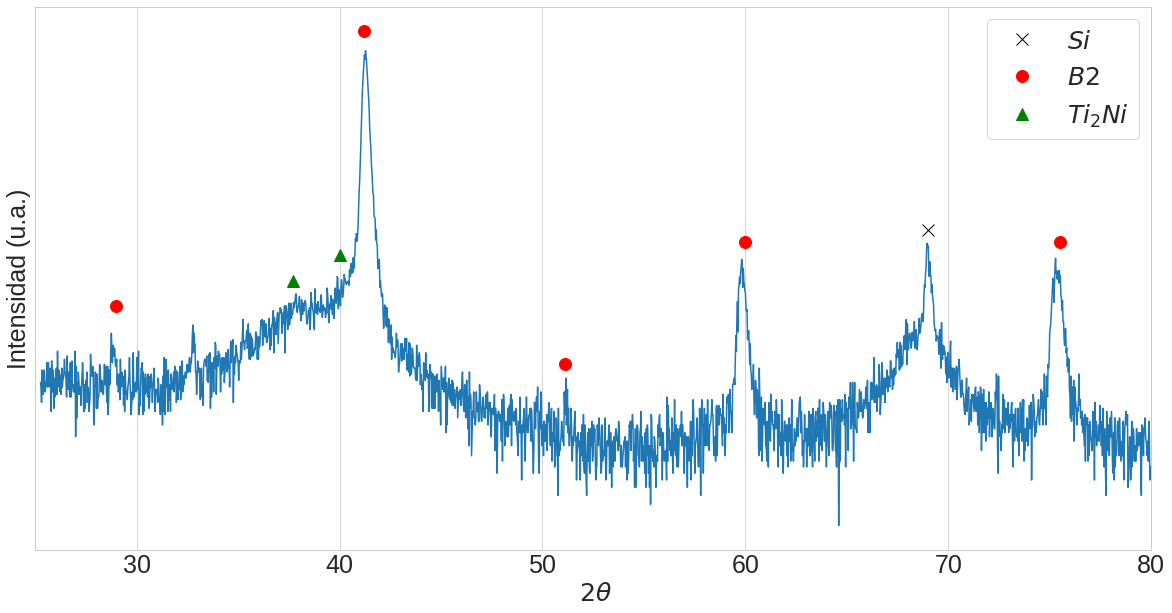
\includegraphics[scale=0.2]{img/RX/NiPoor_500.png}} 
\subfloat[Muestra a $600 ^\circ C$]{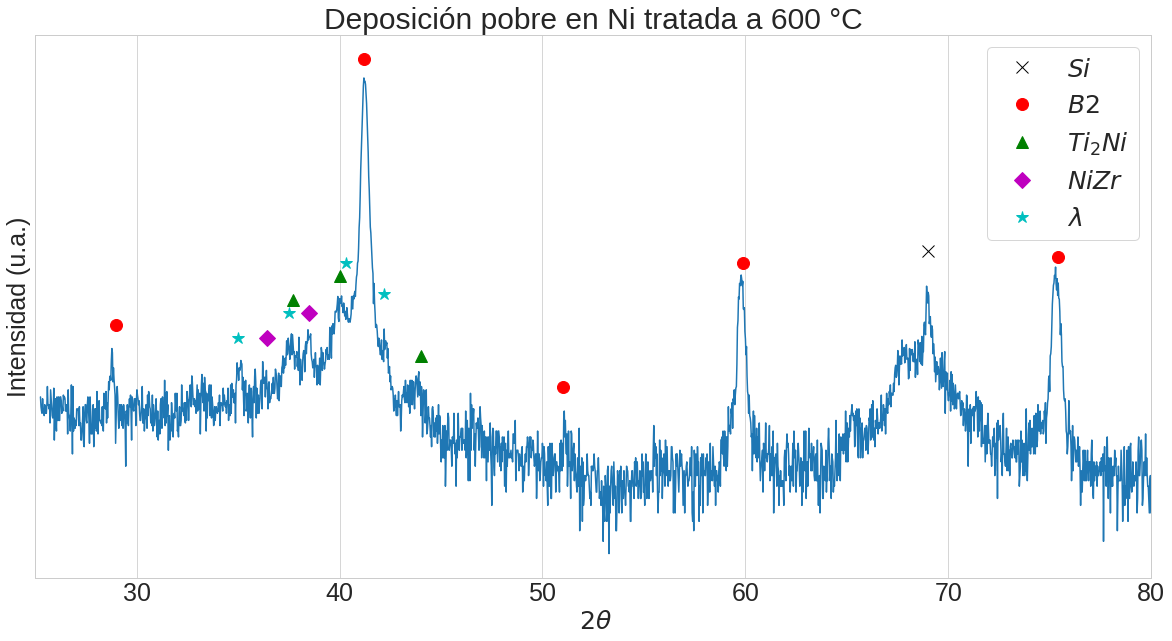
\includegraphics[scale=0.2]{img/RX/NiPoor_600.png}} \\
\subfloat[Muestra a $700 ^\circ C$]{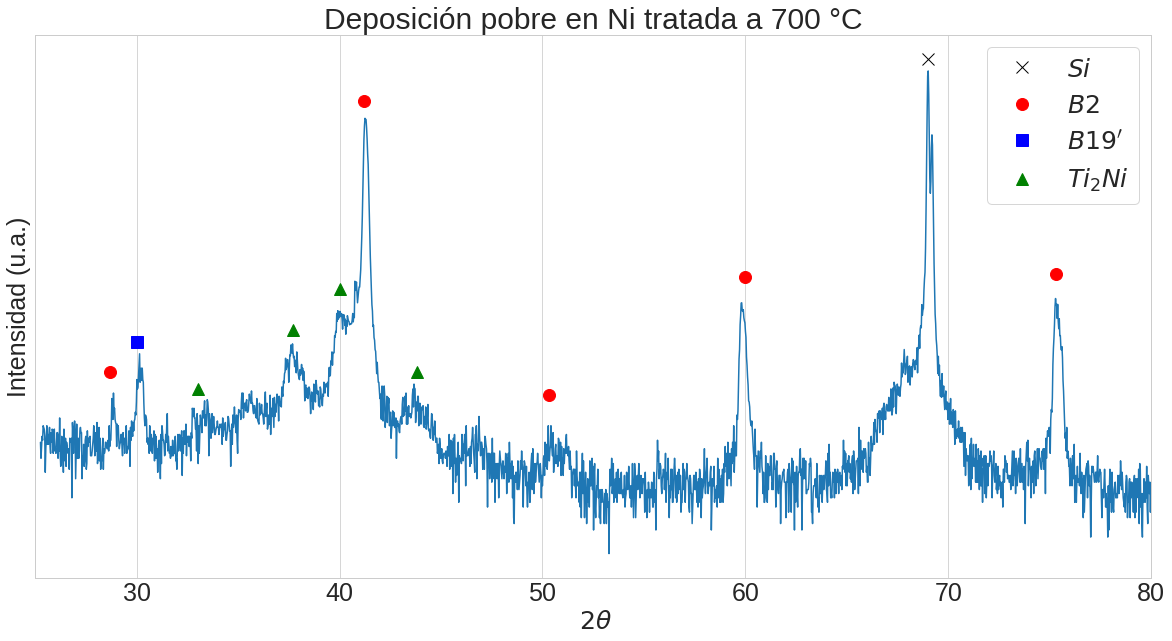
\includegraphics[scale=0.2]{img/RX/NiPoor_700.png}}
\subfloat[Muestra a $800 ^\circ C$]{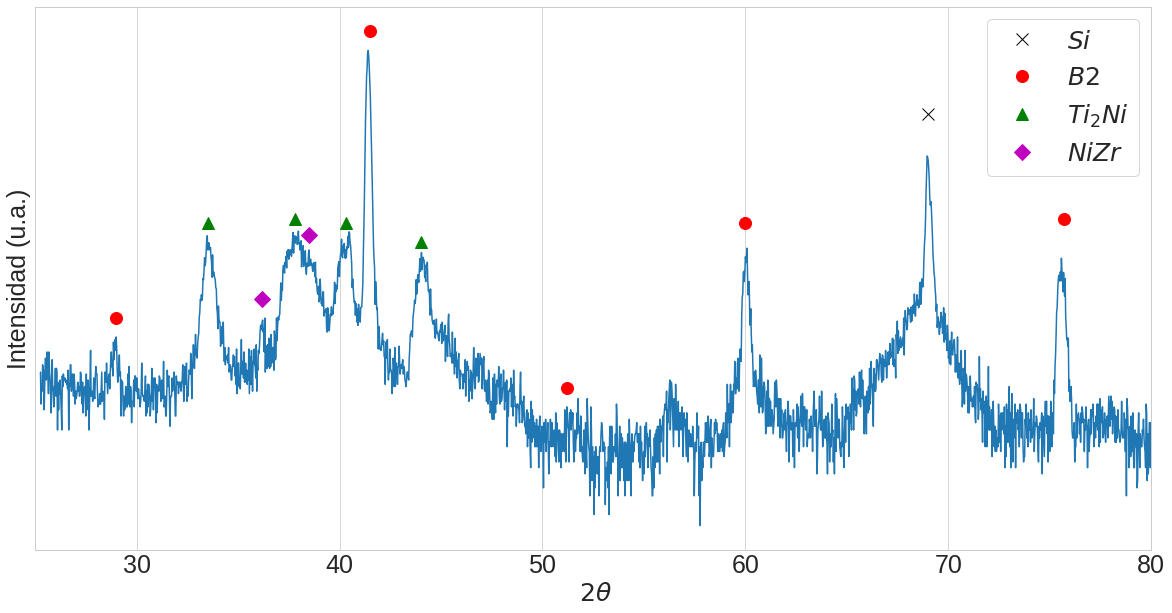
\includegraphics[scale=0.2]{img/RX/NiPoor_800.png}} \\
\caption{Patrones de difracción para las muestras pobres en $Ni$.}
\label{RXNiPoor}
\end{figure}

En todos los difractogramas pueden encontrarse la fase B2 junto con la fase $Ti_2Ni$. Sin embargo, en la muestra de 500$^\circ C$ la proporción de la fase $Ti_2 Ni$ es muy baja. Como se explicó en la sección \ref{Ti2Ni}, la estructura cristalina de la fase $Ti_2 Ni$ es muy similar a la de la fase $Ti_4Ni_2O$, por lo cual es muy difícil de diferenciar por rayos X. Al tener una composición pobre en $Ni$, es esperable encontrar la fase termodinámicamente estable $Ti_2 Ni$, mientras que la fase $Ti_4Ni_2O$ podría aparecer por la oxidación en los tratamientos térmicos.

En la muestra tratada a $600 ^\circ C$, además de las dos fases mencionadas, se observan picos correspondientes a la fase $NiZr$ y a la fase lambda. Por el contrario, en la muestra tratada a $700 ^\circ C$ no se observan picos correspondientes a estas dos fases, pero se observan picos correspondientes a la fase martensítica $B19'$. Esto implica que en esta muestra, a temperatura ambiente, coexisten las fases austenítica y martensítica.

En la muestra tratada a $800 ^\circ C$, vuelven a observarse picos correspondientes a $NiZr$ y crecen los picos de $Ti_2 Ni$. Es importante notar que esta muestra, al ser la tratada a mayor temperatura, presentó una mayor oxidación superficial luego del tratamiento térmico. 


\subsubsection{Imágenes obtenidas por TEM}
\label{TemNiPoorResults}

En la Figura \ref{TEMNiPoor} se presentan las imágenes de TEM de las muestras tratadas a diferentes temperaturas en composición pobre en $Ni$. En la lámina tratada a $500 ^\circ C$ se observa una microestructura caracterizada por granos entre los 10 y 50 $nm$. Mientras que en la lámina tratada a $600 ^\circ C$ se observa una distribución bimodal de grano, con granos de un tamaño entre 110 y 140 $nm$, rodeados por granos mas pequeños de entre 10 y 30 $nm$. En la lámina tratada a $700 ^\circ C$ se observa una distribución de granos mas homogénea con un tamaño de grano promedio de 90 $nm$ y algunos precipitados muy pequeños en borde de grano. Por último, en la muestra tratada a $800 ^\circ C$ se observa una distribución de tamaño de grano más amplia, con granos de entre 20 y 130 $nm$.

\begin{figure}[H]
\centering
\subfloat[Muestra a $500 ^\circ C$]{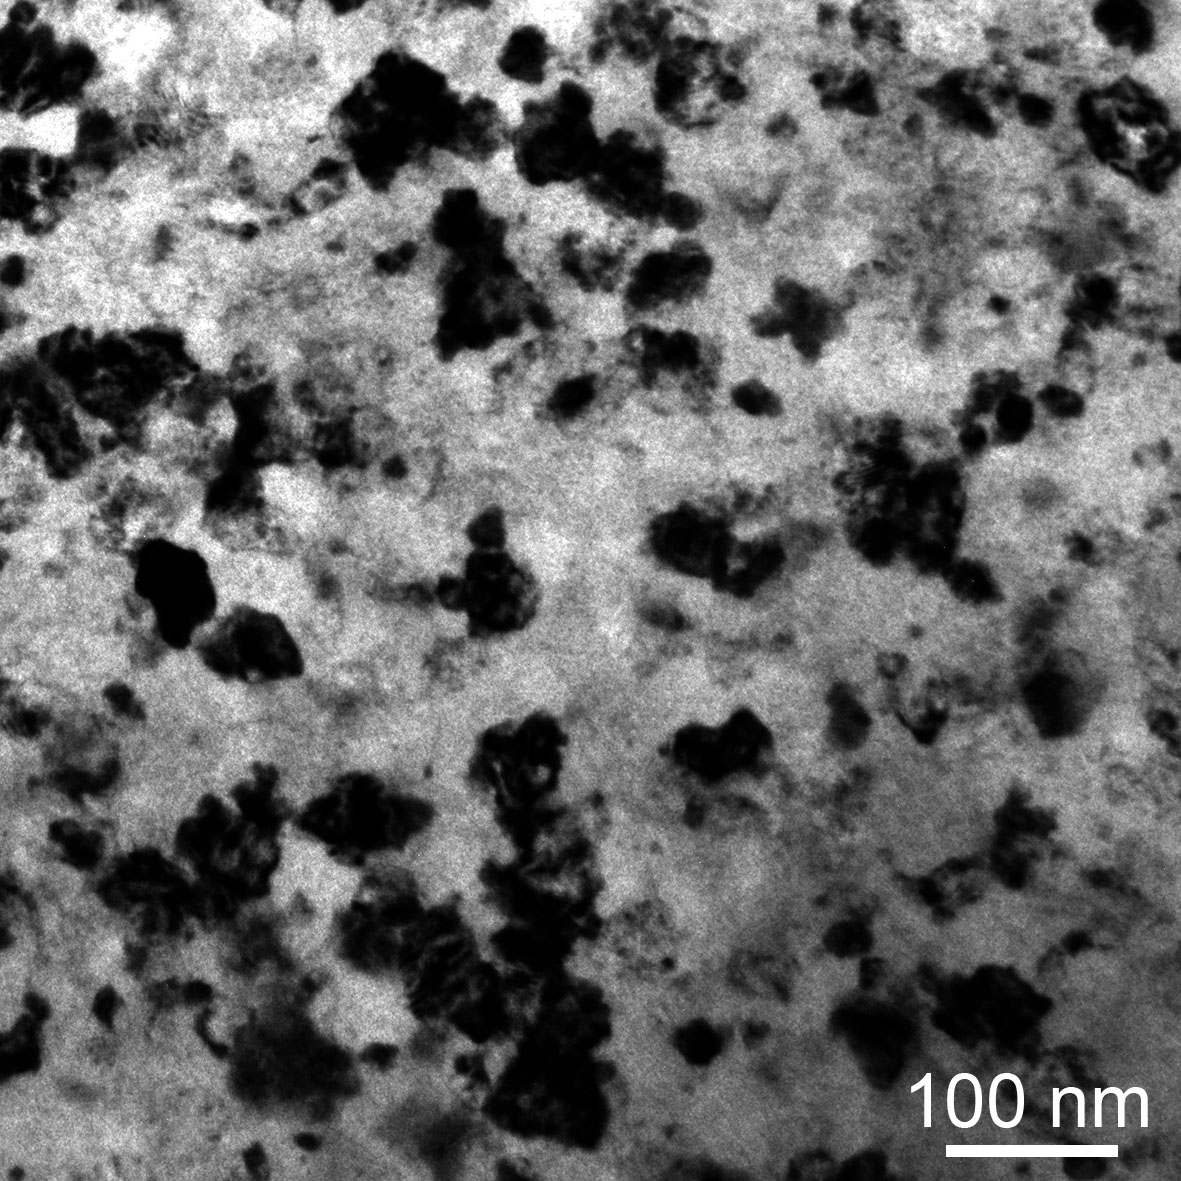
\includegraphics[scale=0.6]{img/TEM/Fig24a.jpg}} 
\subfloat[Muestra a $600 ^\circ C$]{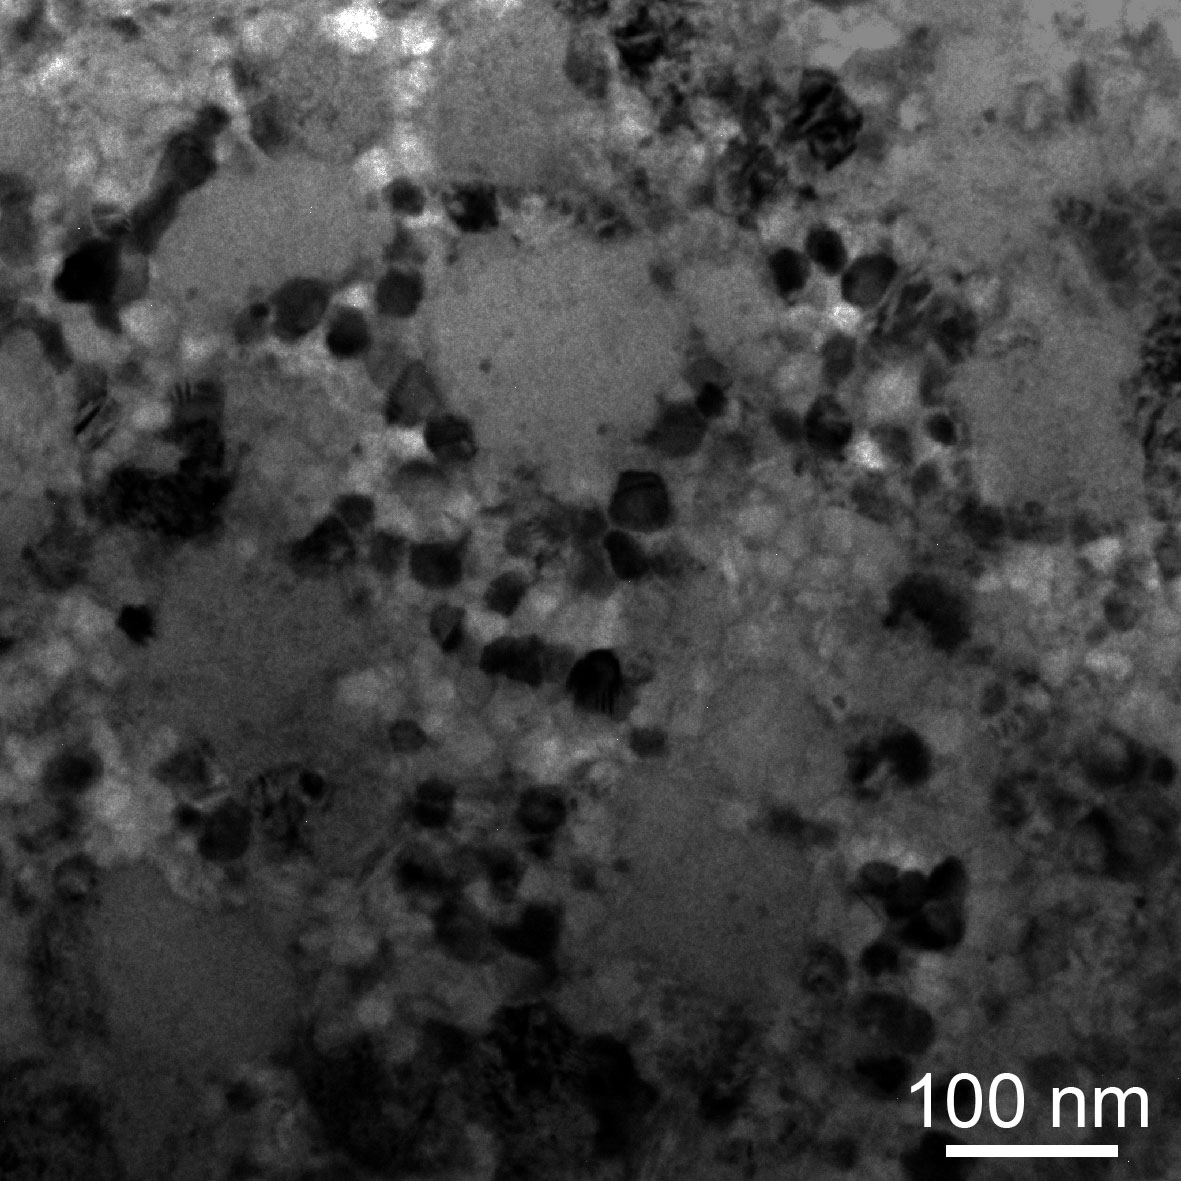
\includegraphics[scale=0.6]{img/TEM/Fig24b.jpg}} \\
\subfloat[Muestra a $700 ^\circ C$]{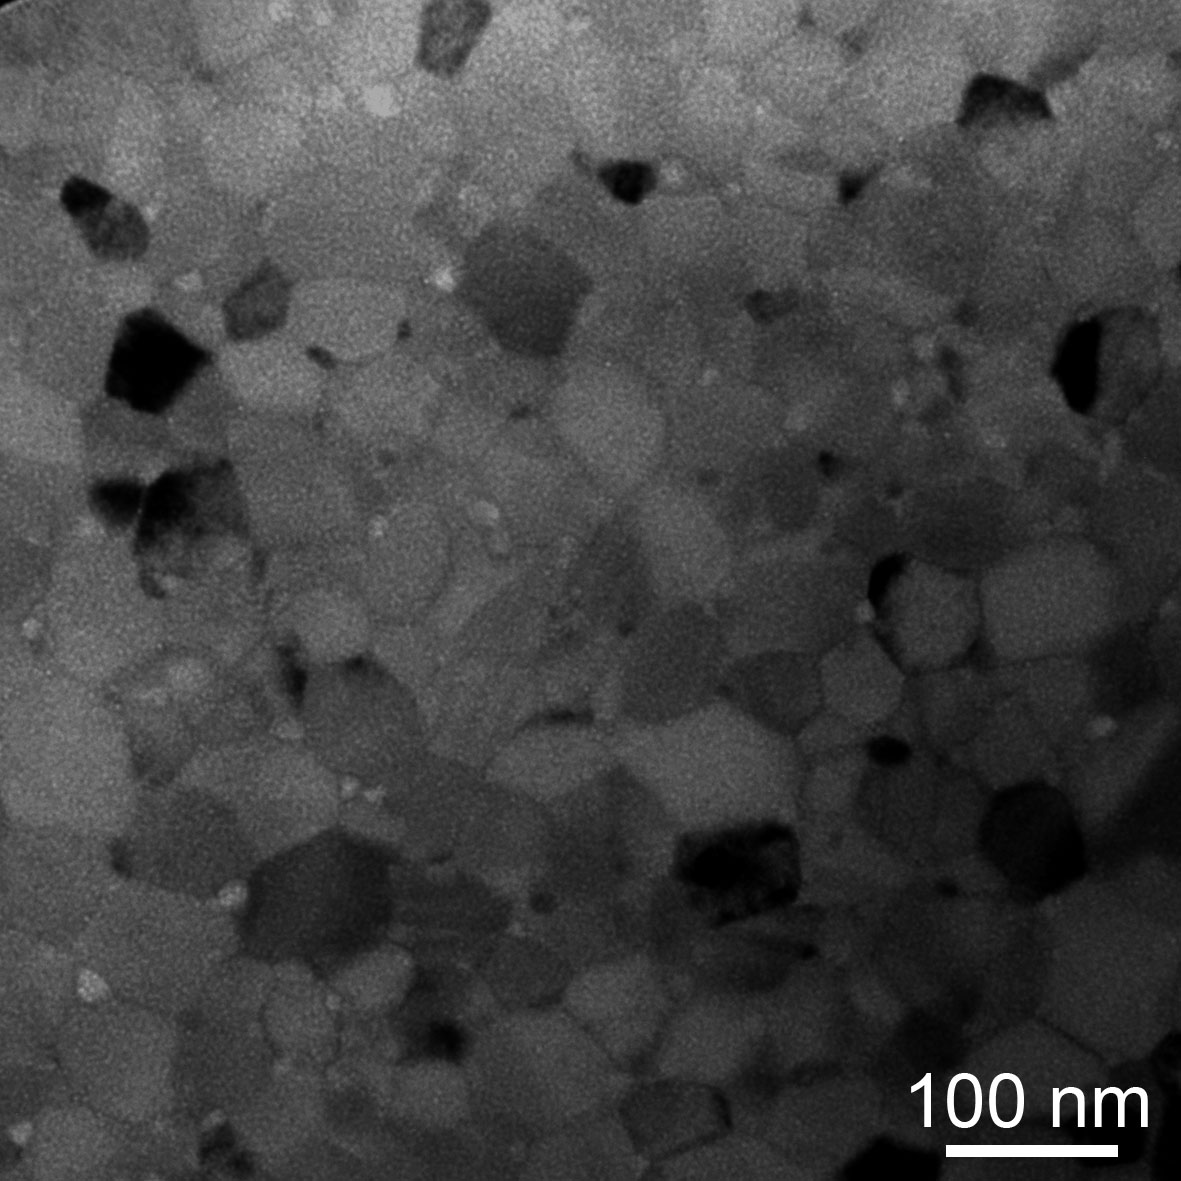
\includegraphics[scale=0.6]{img/TEM/Fig24c.jpg}} 
\subfloat[Muestra a $800 ^\circ C$]{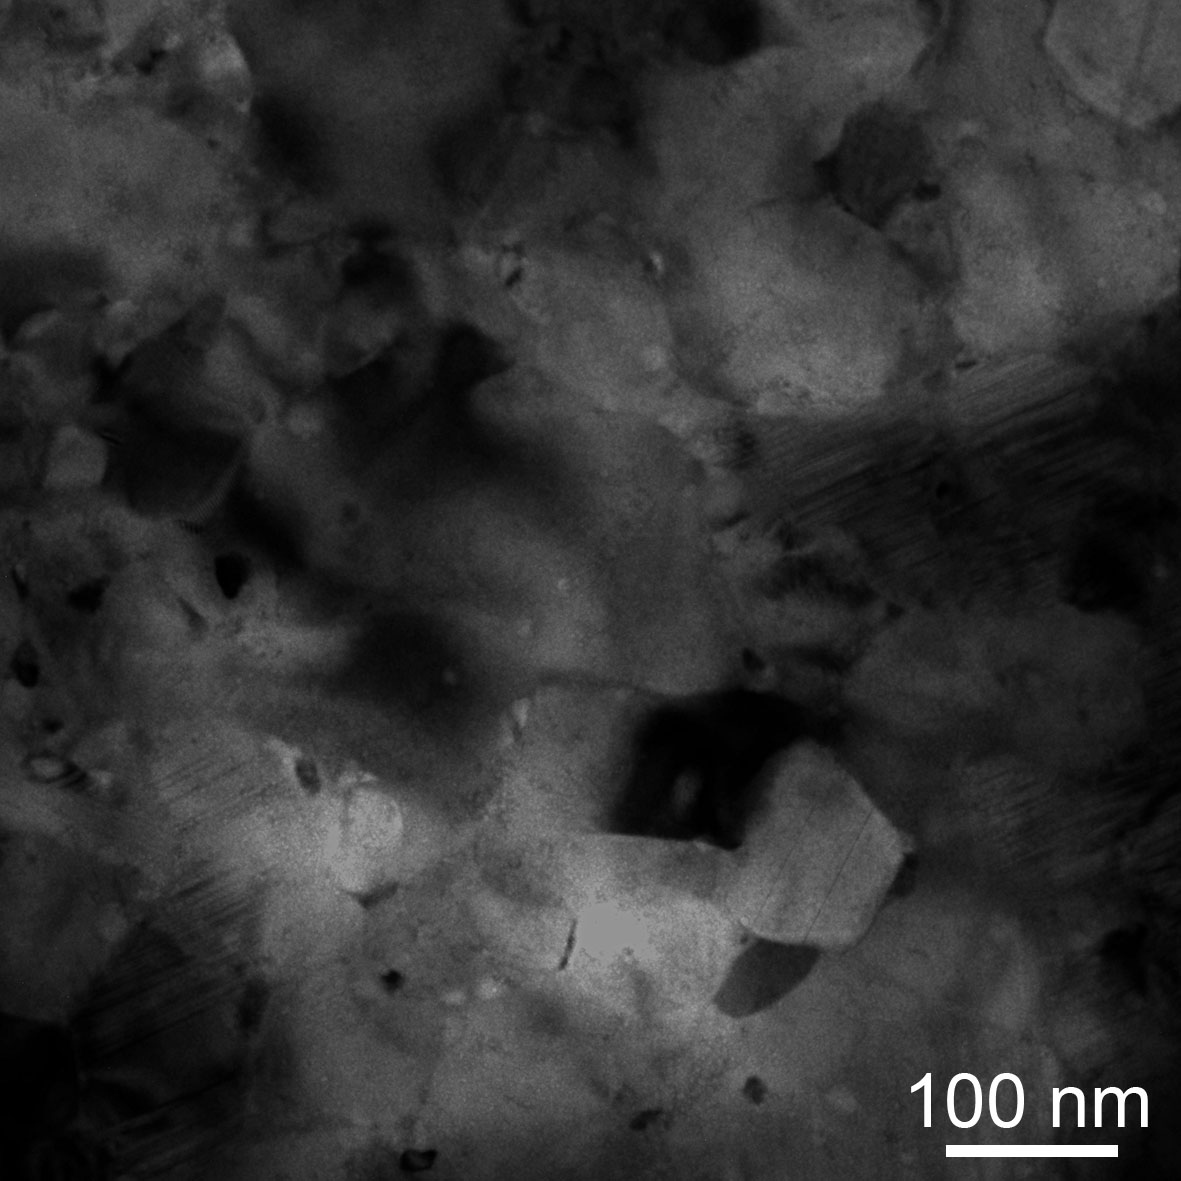
\includegraphics[scale=0.6]{img/TEM/Fig24d.jpg}}
\caption{Imágenes de TEM para las muestras pobres en $Ni$.}
\label{TEMNiPoor}
\end{figure}

En la Figura \ref{TEMNiPoor-PD}(a) se observa un patrón de difracción de anillos obtenidos para la muestra tratada a $500 ^\circ C$, el cual fue indexado teniendo en cuenta las fases B2 y $Ti_2Ni$. Mientras que en la Figura \ref{TEMNiPoor-PD}(b) se muestra una imagen de campo claro de la lámina tratada a $600 ^\circ C$, donde se observa un grano de aproximadamente 120 $nm$ orientado en la dirección [001], el cual corresponde a la fase B2 y conjuntamente se presenta el patrón de difracción de anillos obtenido para de los granos más pequeños, en la cual se muestran indexados solo los anillos más importantes de la fase $Ti_2 Ni$. Esto muestra que la distribución bimodal de tamaño de grano de esta lámina se debe a la cristalización de estas dos fases en regiones adyacentes. El patrón de anillos presentado en la Figura \ref{TEMNiPoor-PD}(c) fue obtenido en la muestra tratada a $700 ^\circ C$, y fue  indexado con las fases B2 y $Ti_2Ni$. Es importante notar que se puede observar algún anillo sin indexar, sin embargo resultó difícil establecer a qué fase corresponde. Finalmente en la Figura \ref{TEMNiPoor-PD}(d) se muestra un grano de la fase $Ti_2Ni$, observado en la lámina tratada a $800 ^\circ C$, cuyo tamaño superó los $\sim 100 nm$ (patrón de difracción en el eje de zona [112]).

\begin{figure}[H]
\centering
\subfloat[Muestra a $500 ^\circ C$]{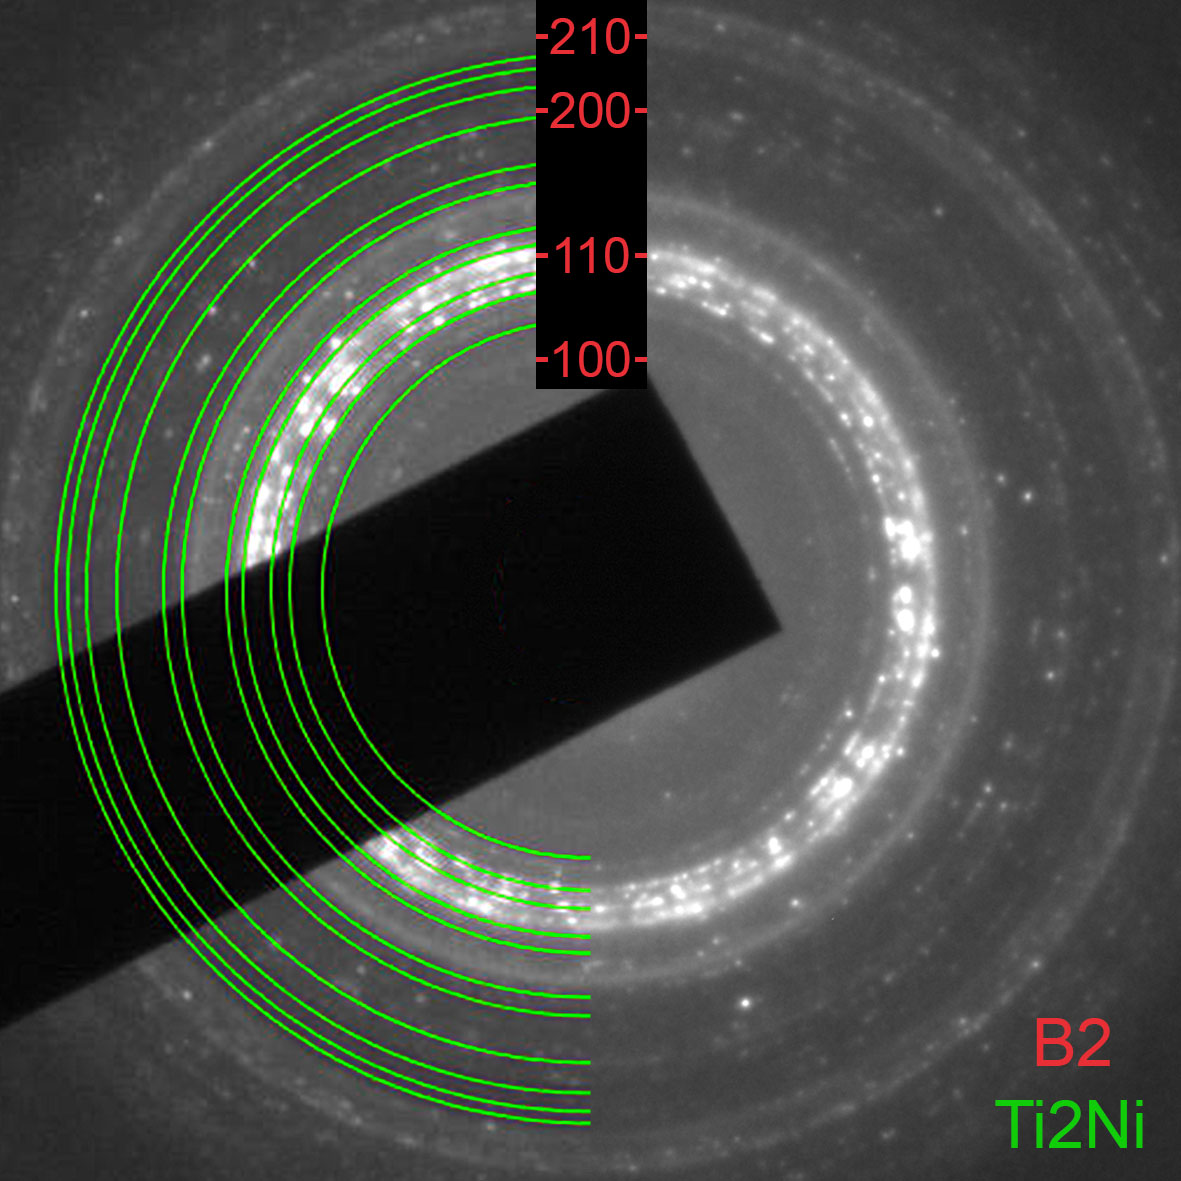
\includegraphics[scale=0.6]{img/TEM/Fig25a.jpg}} 
\subfloat[Muestra a $600 ^\circ C$]{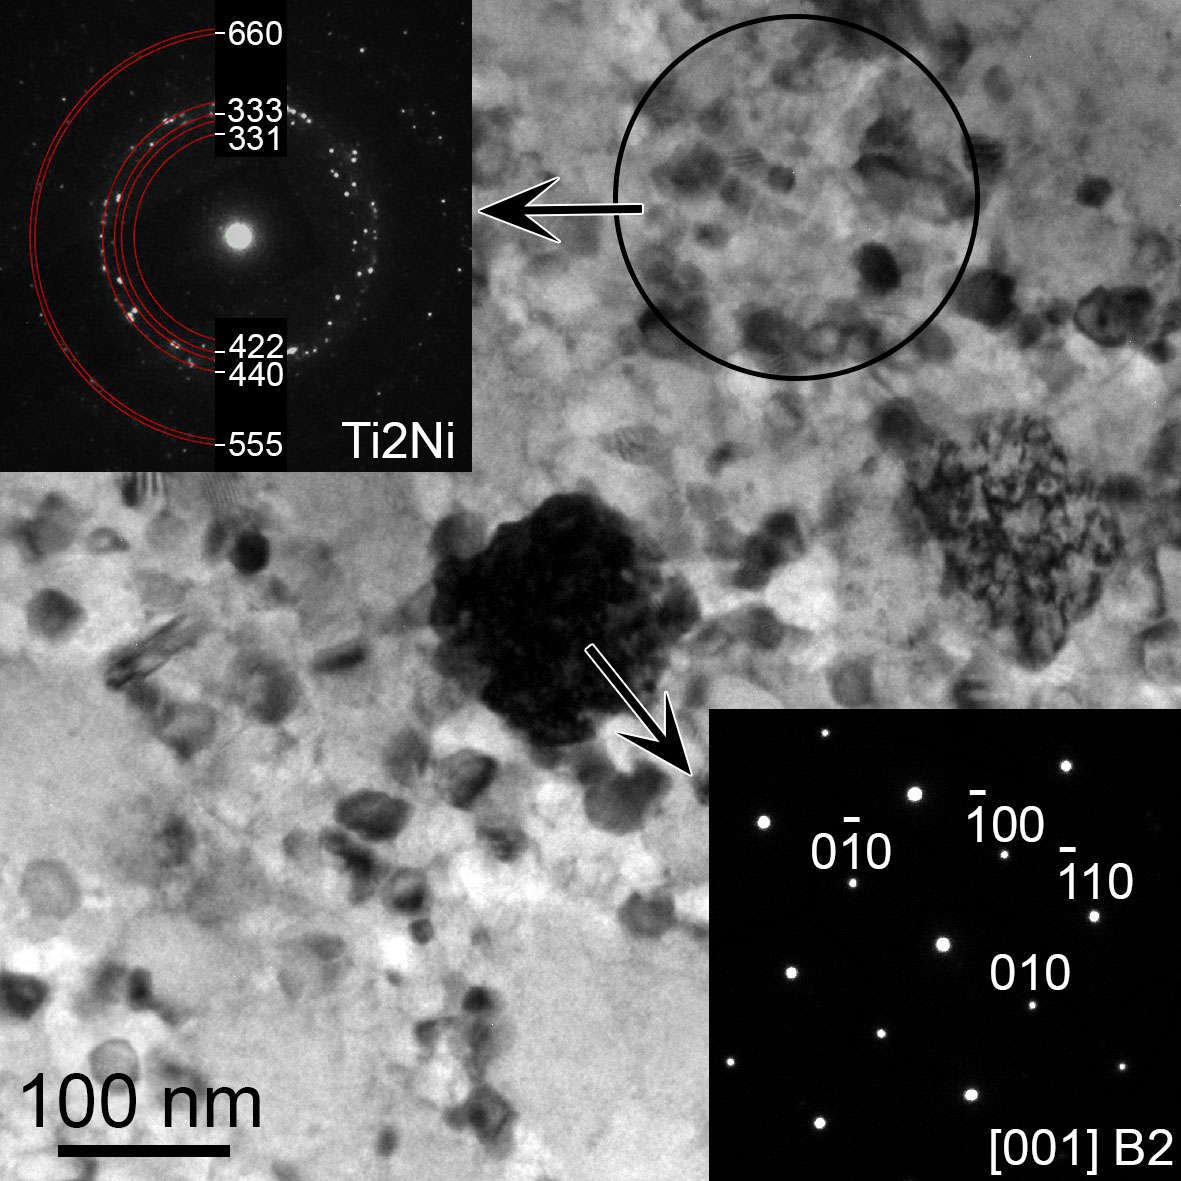
\includegraphics[scale=0.6]{img/TEM/Fig25b.jpg}} \\
\subfloat[Muestra a $700 ^\circ C$]{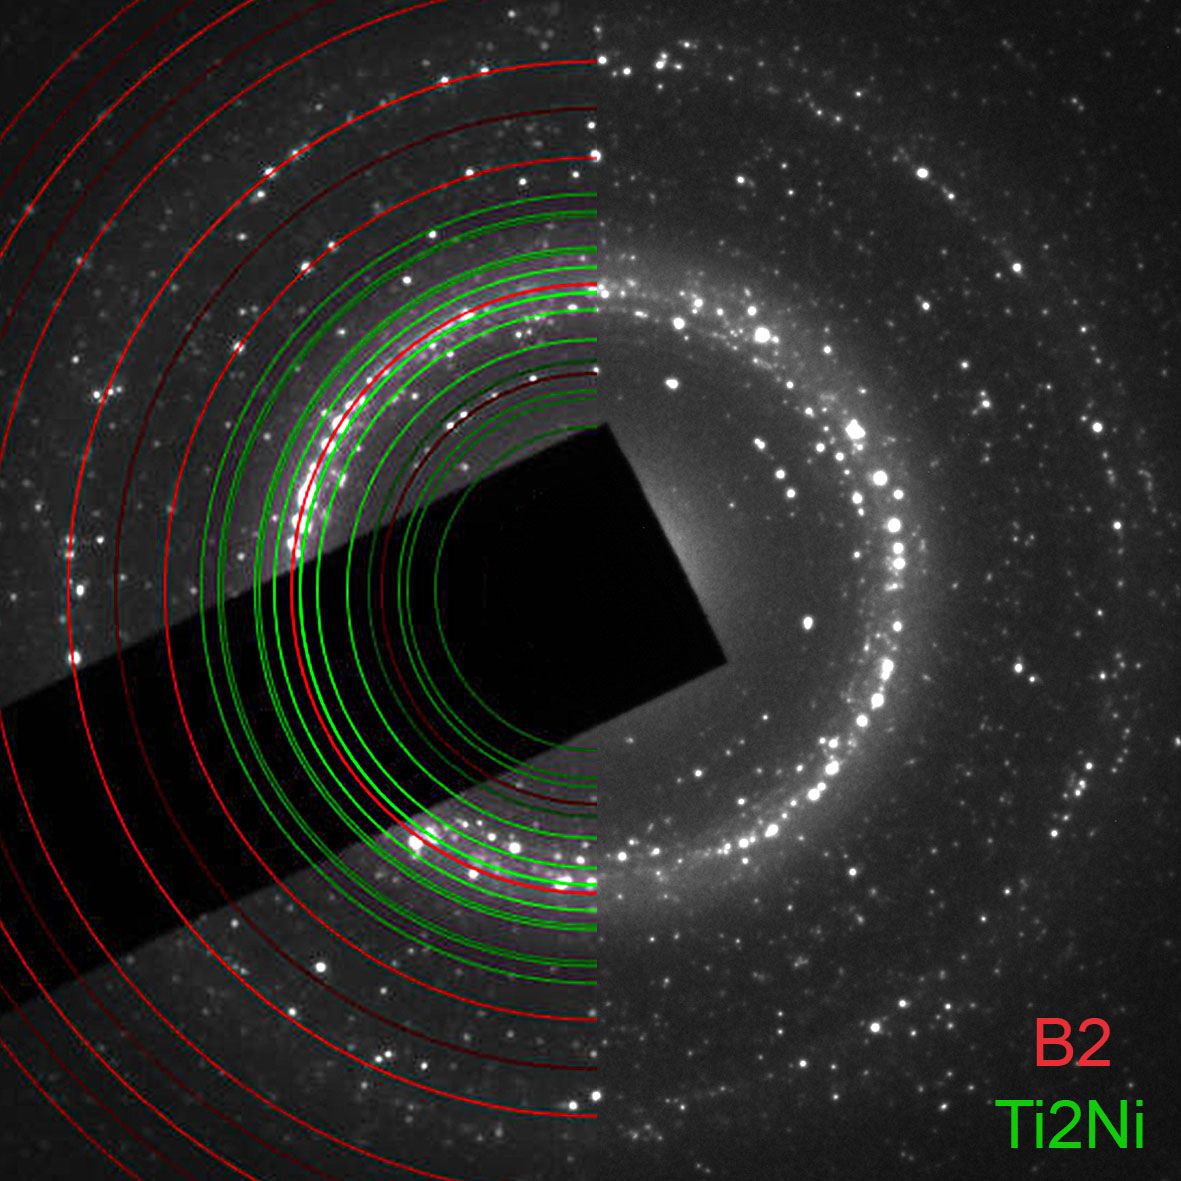
\includegraphics[scale=0.6]{img/TEM/Fig25c.jpg}} 
\subfloat[Muestra a $800 ^\circ C$]{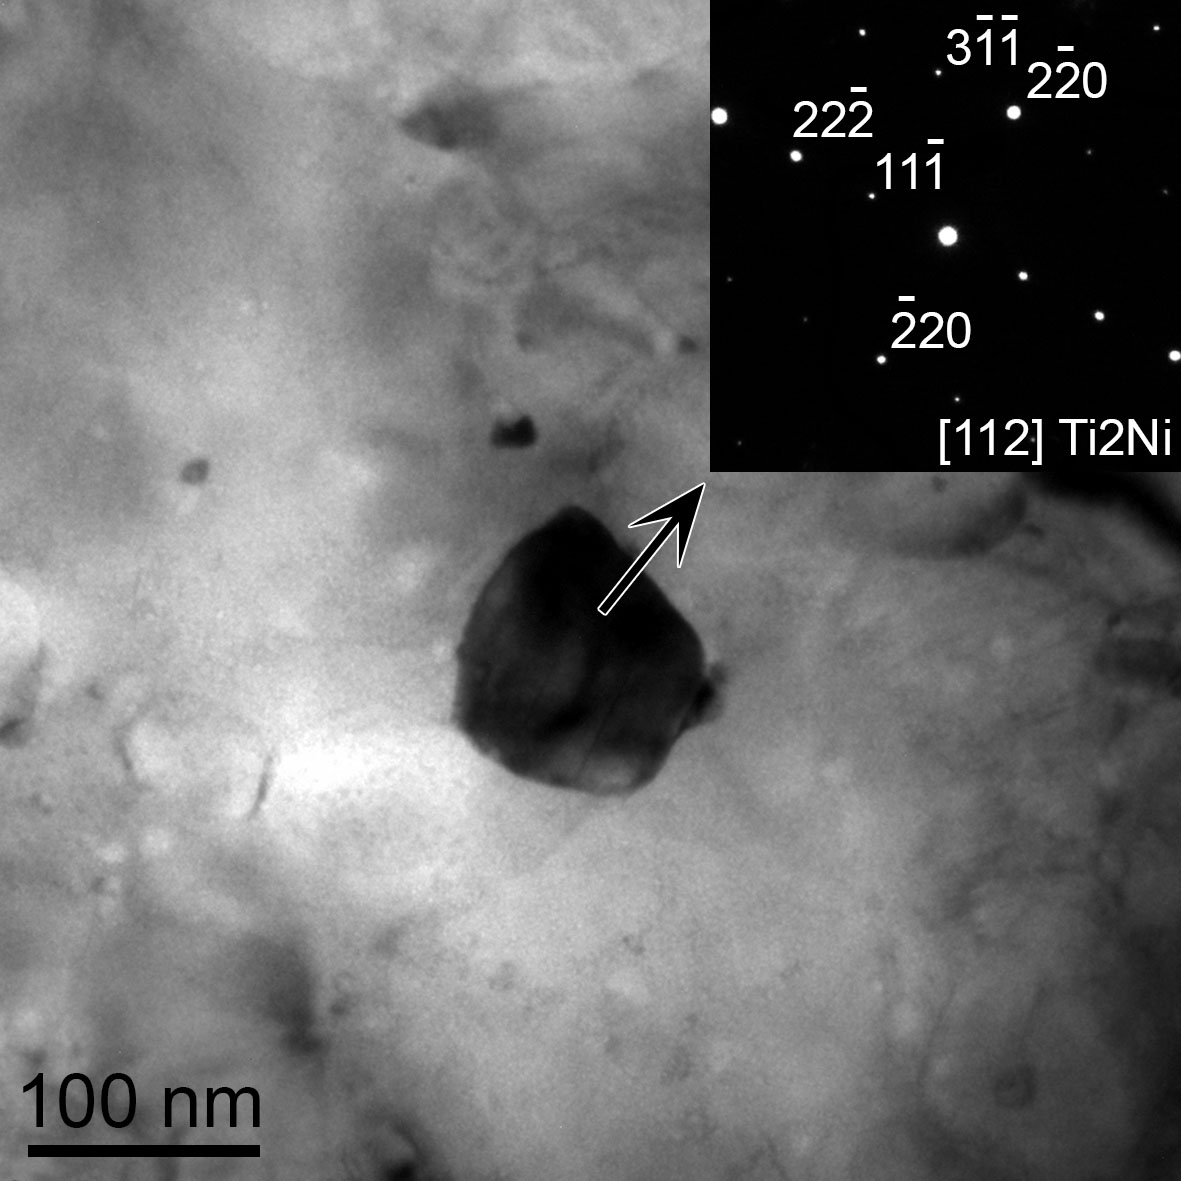
\includegraphics[scale=0.6]{img/TEM/Fig25d.jpg}} 
\caption{Patrones de difracción de TEM para las muestras pobres en $Ni$.}
\label{TEMNiPoor-PD}
\end{figure}

\subsubsection{Transformación martensítica}

Para estudiar la transformación martensítica se realizó un estudio de calorimetría diferencial de barrido en las muestras sometidas a los distintos tratamientos térmicos. En este caso no fue posible realizar el método de resistividad por cuatro puntas ya que las láminas eran extremadamente frágiles, impidiendo utilizar los contactos por presión de dicho dispositivo.

Analizando las curvas de calentamiento y enfriamiento, mostradas en la Figura \ref{DSCNiPoor}, no es posible apreciar una transformación de fase. Esto se puede deber a que la cantidad de masa que transforma es baja y que la transformación está extendida en un amplio rango de temperatura. Esta discusión será retomada en la sección \ref{TransfomacionDiscusion}. La descripción de cómo fueron obtenidas estas curvas a partir de las mediciones originales se explica en la sección \ref{BaseLineAppendix}.

\begin{figure}[H]
\noindent\makebox[\linewidth][c]{
	\subfloat[Muestra tratada a $500 ^\circ C$]{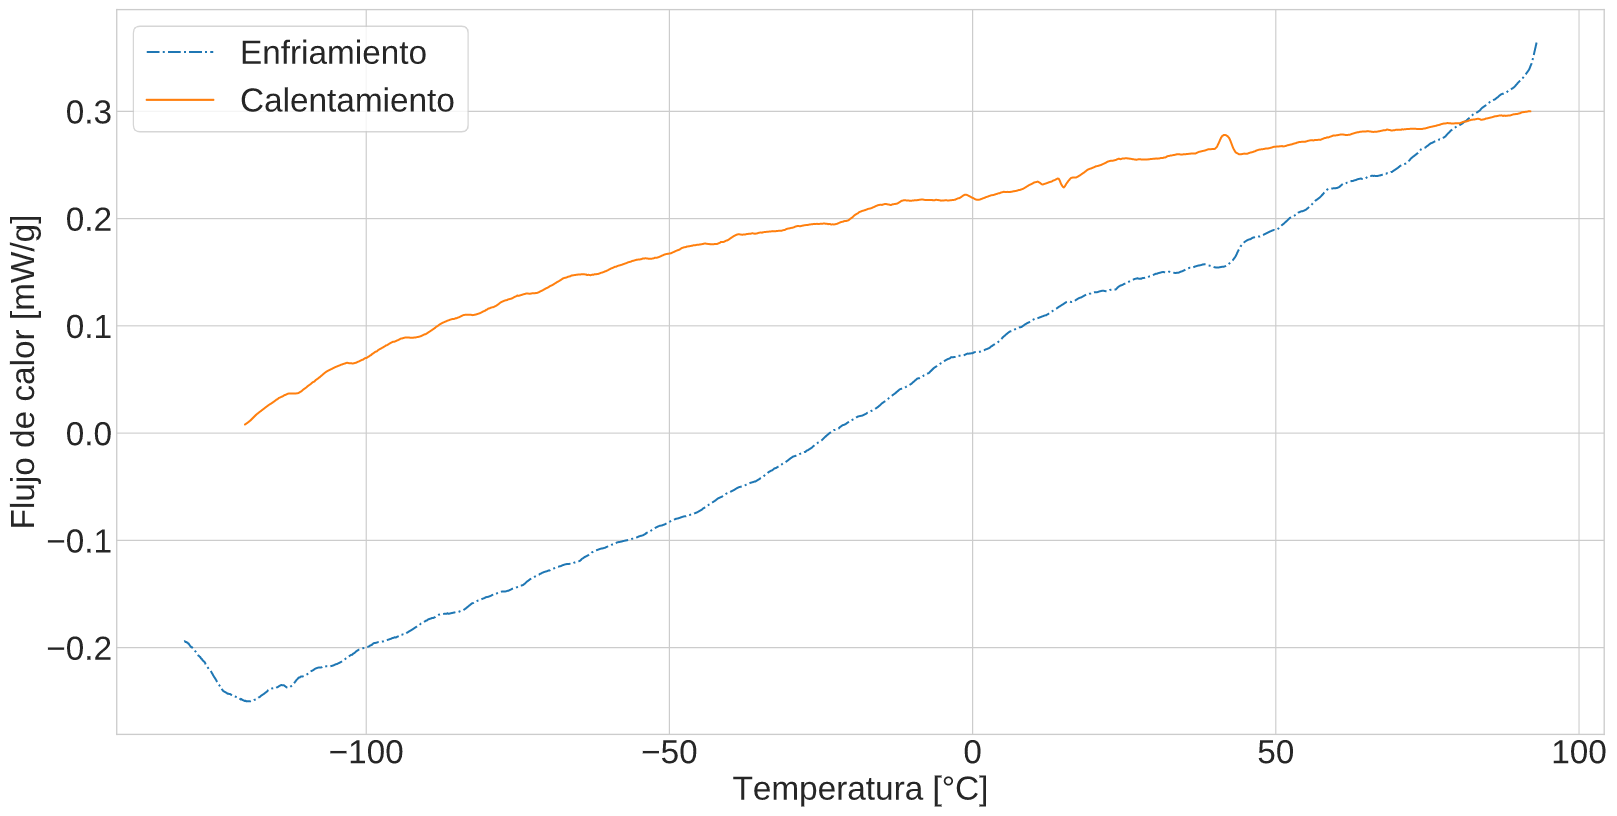
\includegraphics[scale=0.13]{img/DSCNiPoor/500}}
	\subfloat[Muestra tratada a $600 ^\circ C$]{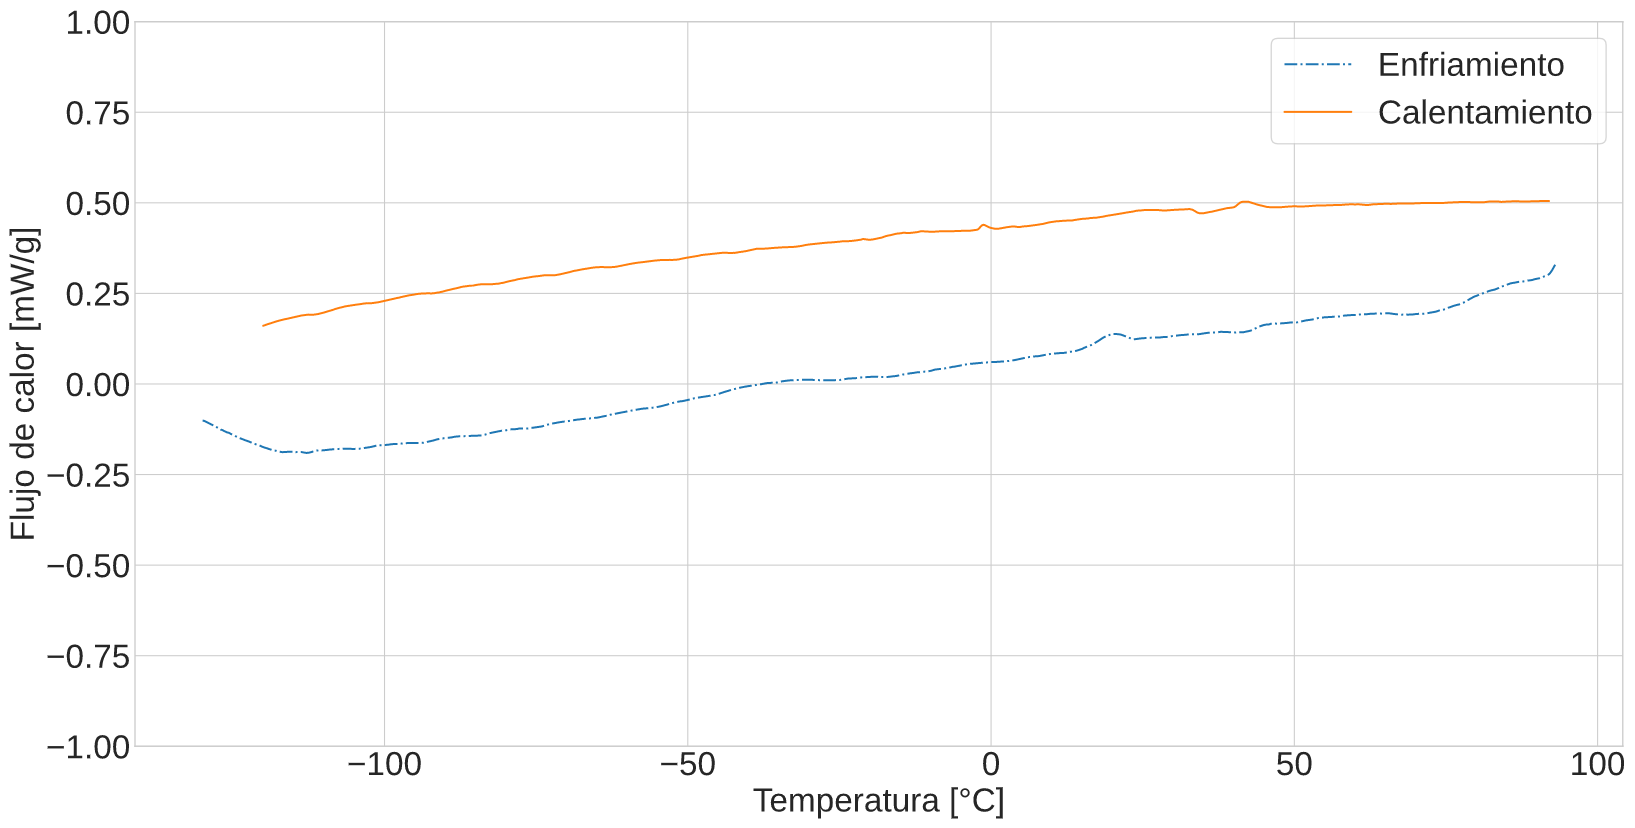
\includegraphics[scale=0.13]{img/DSCNiPoor/600}}} \\
\noindent\makebox[\linewidth][c]{
	\subfloat[Muestra tratada a $700 ^\circ C$]{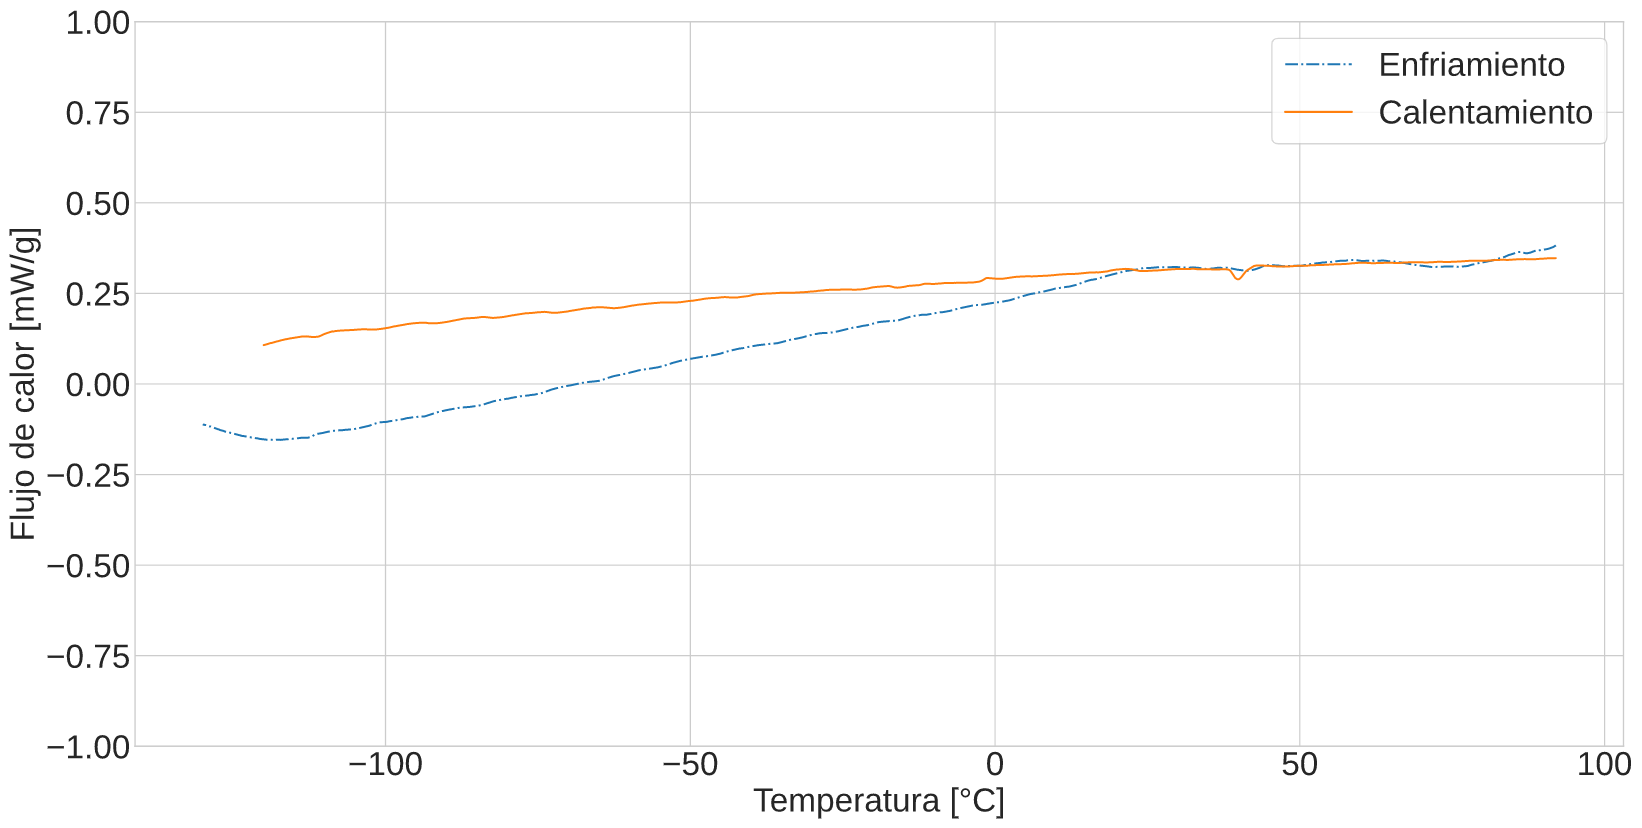
\includegraphics[scale=0.13]{img/DSCNiPoor/700}}
	\subfloat[Muestra tratada a $800 ^\circ C$]{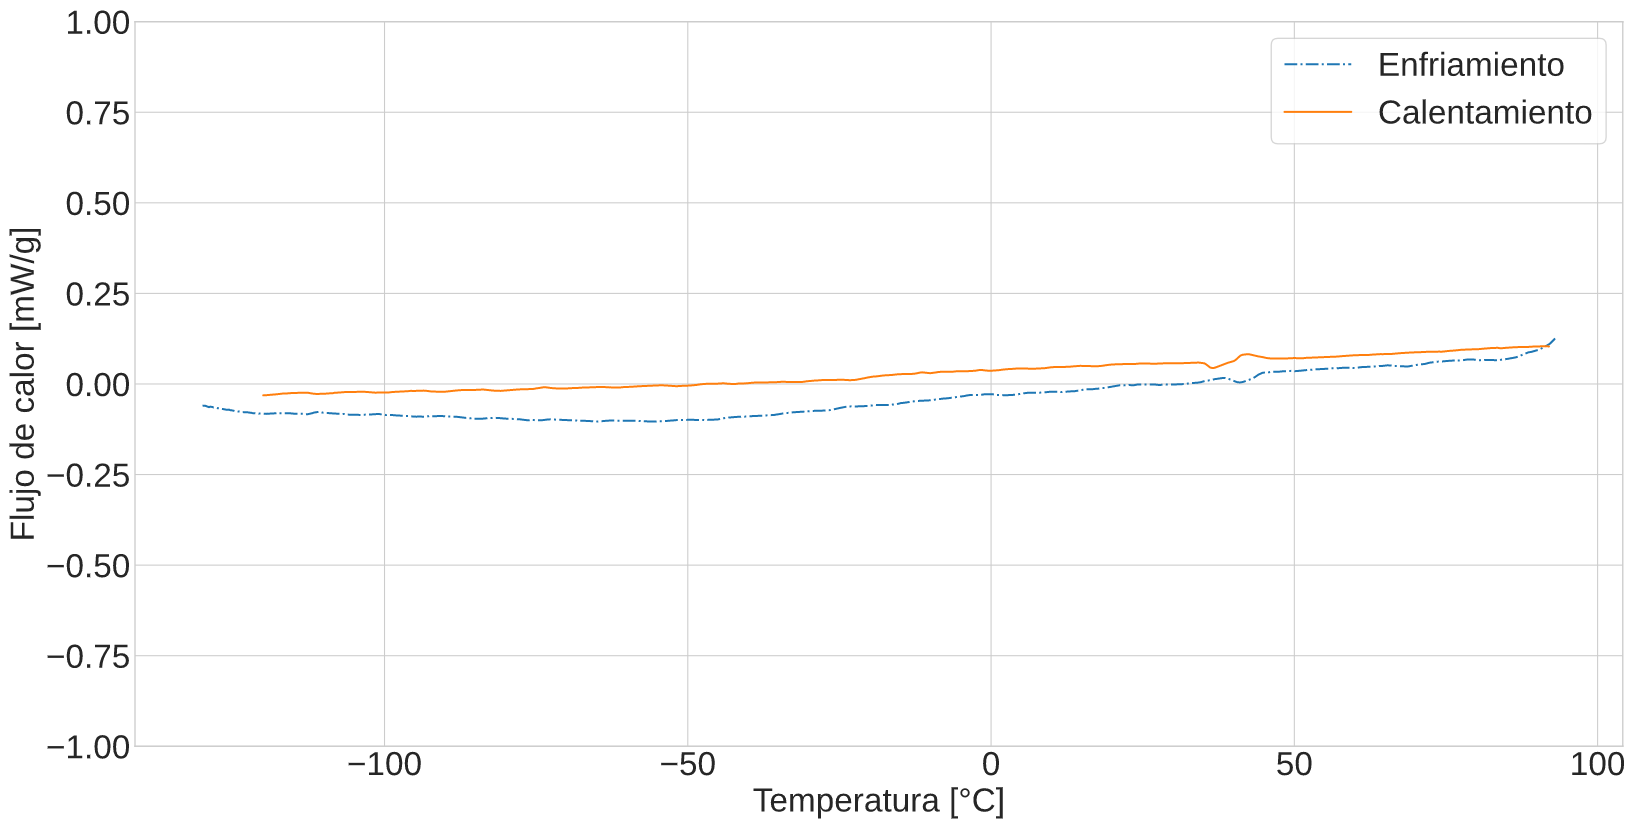
\includegraphics[scale=0.13]{img/DSCNiPoor/800}}}
\caption{Curvas de DSC para las distintas muestras.}
\label{DSCNiPoor}
\end{figure}


\subsection{Deposición rica en $Ni$}
\subsubsection{Fases obtenidas}
En la Figura \ref{RXNiRich} se muestran los difractogramas de las láminas ricas en $Ni$ con los distintos tratamientos térmicos. En dichas figuras se muestra el logaritmo natural de la intensidad, de modo que todos los picos puedan ser apreciados. Del mismo modo que en las muestras pobres en $Ni$, la identificación de las distintas fases se realizó a través de la simulación de las estructuras cristalinas con el programa PowderCell.

\begin{figure}[H]
\subfloat[Muestra a $500 ^\circ C$]{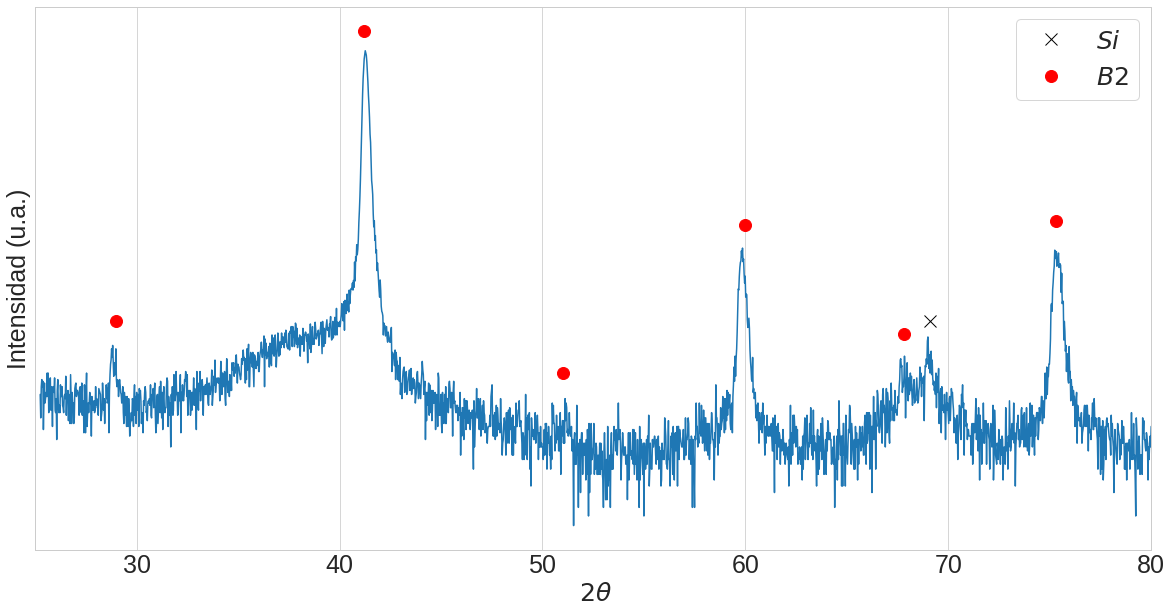
\includegraphics[scale=0.2]{img/RX/NiRich_500.png}}
\subfloat[Muestra a $600 ^\circ C$]{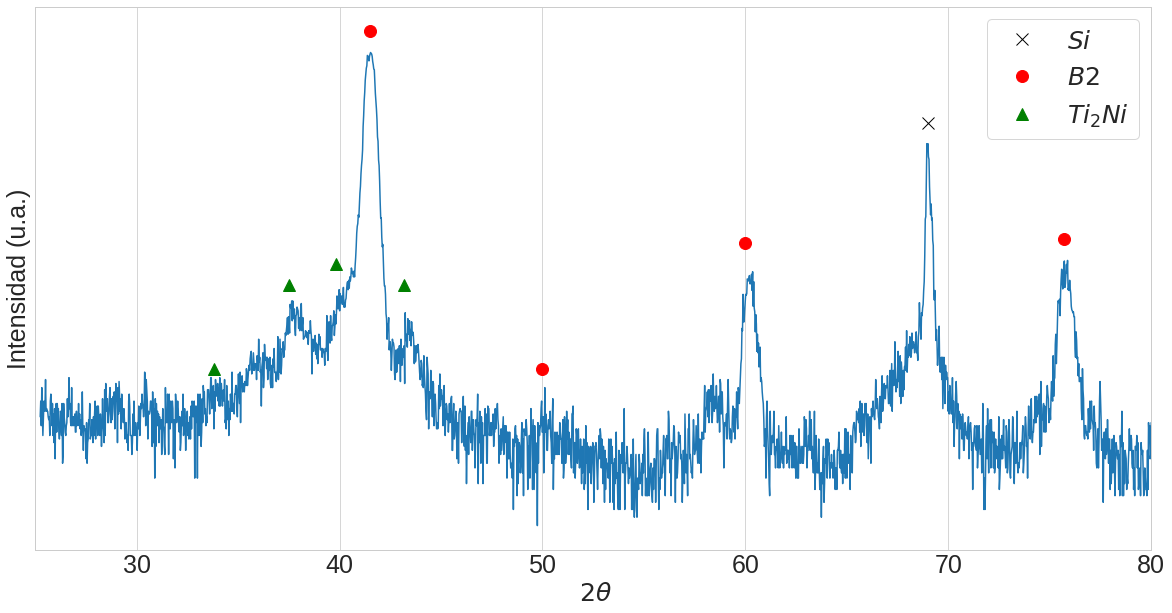
\includegraphics[scale=0.2]{img/RX/NiRich_600.png}} \\
\subfloat[Muestra a $700 ^\circ C$]{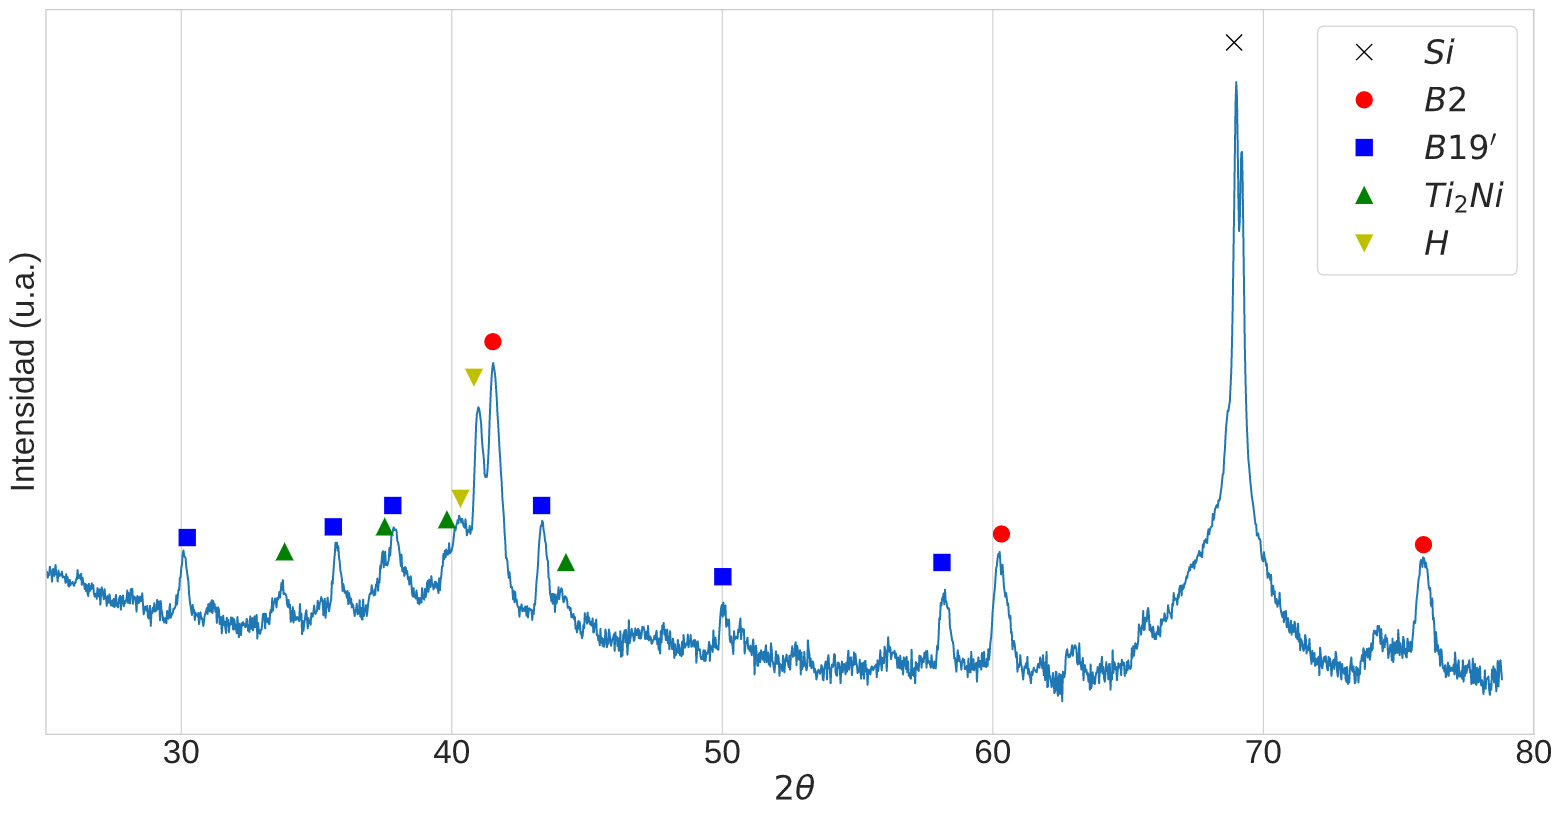
\includegraphics[scale=0.152]{img/RX/NiRich_700.png}} 
\subfloat[Muestra a $800 ^\circ C$]{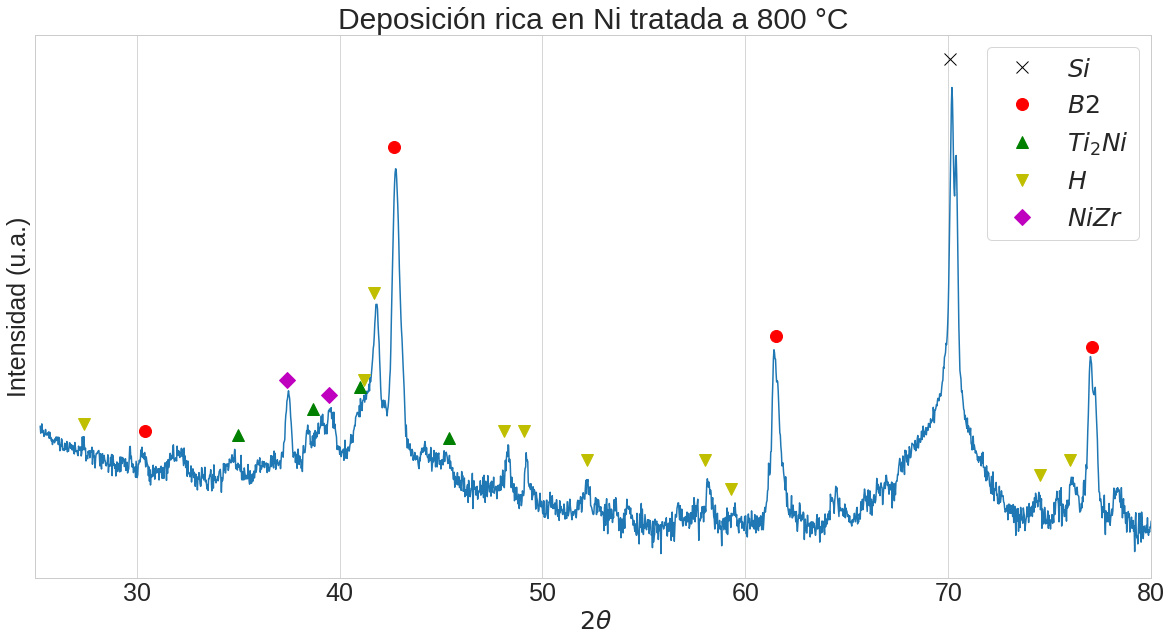
\includegraphics[scale=0.2]{img/RX/NiRich_800.png}} 
\caption{Patrones de difracción de rayos X para las muestras ricas en $Ni$.}
\label{RXNiRich}
\end{figure}

En todos los difractogramas puede encontrarse la fase B2, correspondiente a la austenita, siendo esta la única fase existente en la lámina tratada a $500 ^\circ C$. En los difractogramas de las muestras tratadas a mayores temperaturas comienzan a apreciarse picos de $Ti_2Ni$ (o posible $Ti_4Ni_2O$, ya que sus estructuras son muy similares) y de fase H. Además en la muestra tratada a $700 ^\circ C$ se observa la fase $B19'$, mientras que en la tratada a $800 ^\circ C$ se observa $NiZr$.

\subsubsection{Imágenes obtenidas por TEM}

En la Figura \ref{TEMNiRich} se muestran imágenes obtenidas por TEM para las muestras sometidas a los diferentes tratamientos térmicos de las láminas ricas en $Ni$. En estas figuras se puede observar un ligero aumento del tamaño de grano a medida que aumenta la temperatura del tratamiento térmico entre los $500 ^\circ C$ y $700 ^\circ C$. De esta manera, en la muestra tratada a menor temperatura se observa un tamaño de grano promedio de 70 $nm$, mientras que el tamaño promedio aumenta a 90 $nm$ en la muestra tratada a $600 ^\circ C$ y alcanza los 115 $nm$ en la muestra tratada a $700 ^\circ C$ . Por el otro lado, en la muestra tratada $800 ^\circ C$ se puede observar una distribución más amplia del tamaño de grano, con algunos granos pequeños de decenas de nanómetro, hasta granos de dimensiones superiores a los 500 $nm$. 

\begin{figure}[H]
\centering
\subfloat[Muestra a $500 ^\circ C$]{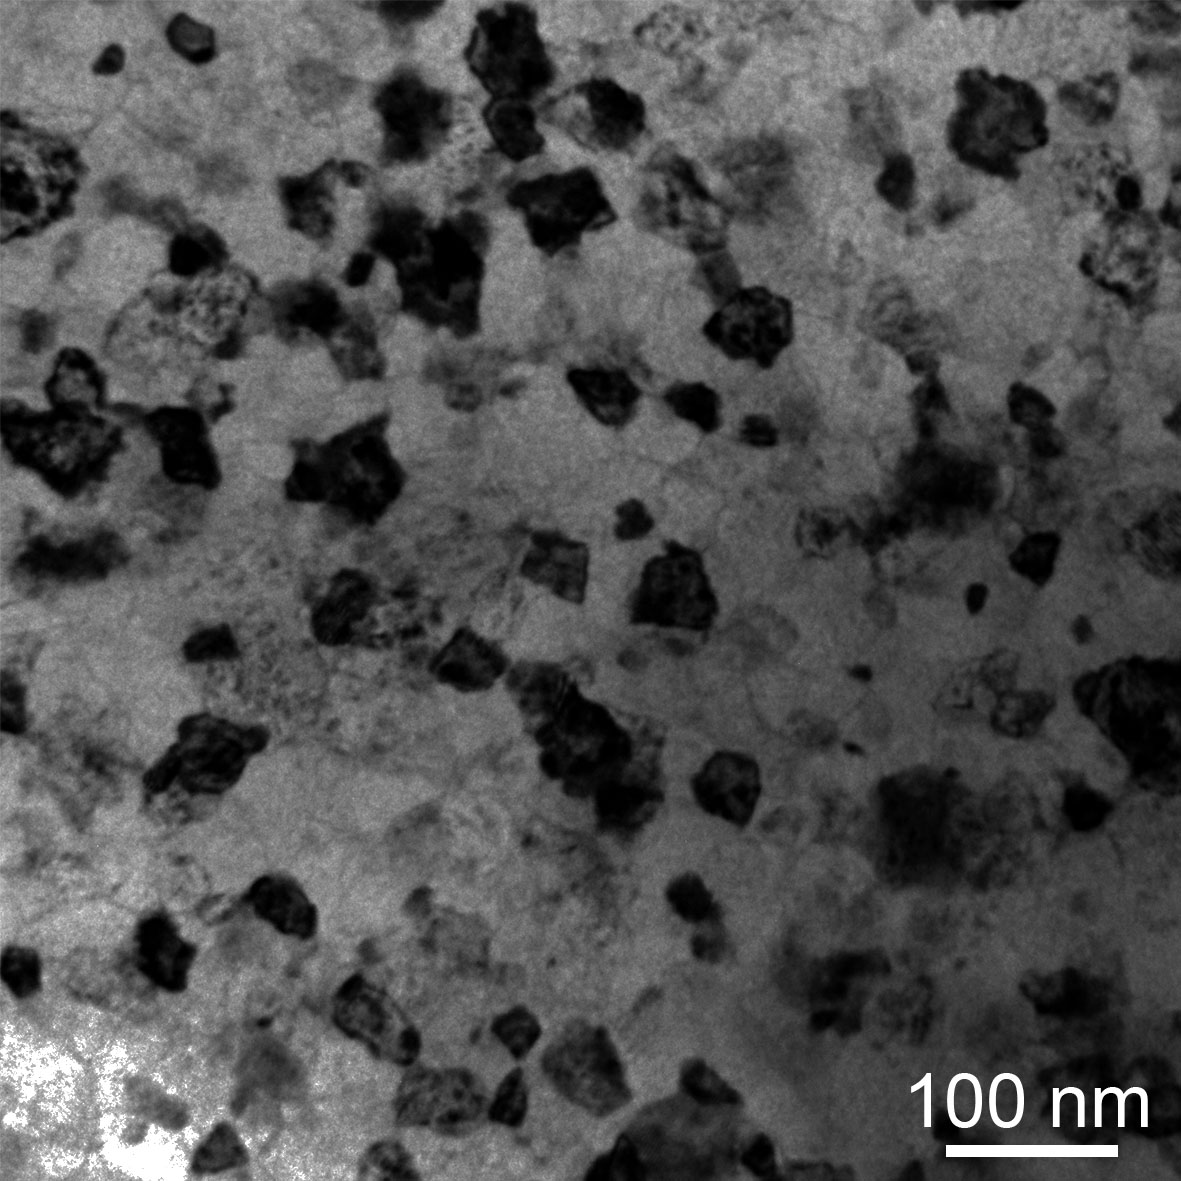
\includegraphics[scale=0.6]{img/TEM/Fig27a.jpg}} 
\subfloat[Muestra a $600 ^\circ C$]{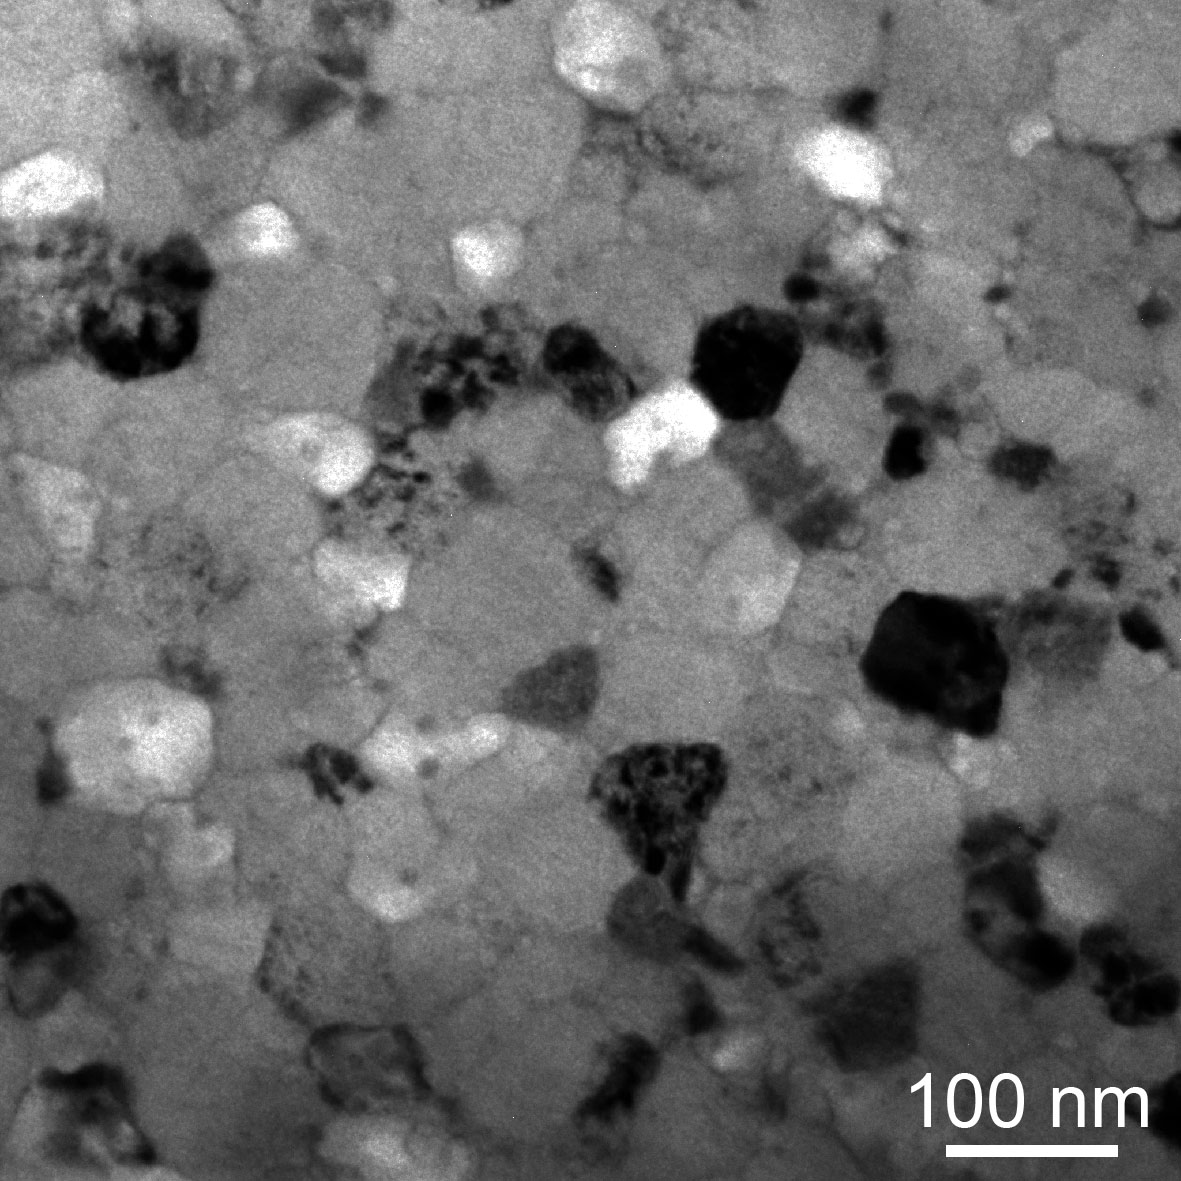
\includegraphics[scale=0.6]{img/TEM/Fig27b.jpg}} \\
\subfloat[Muestra a $700 ^\circ C$]{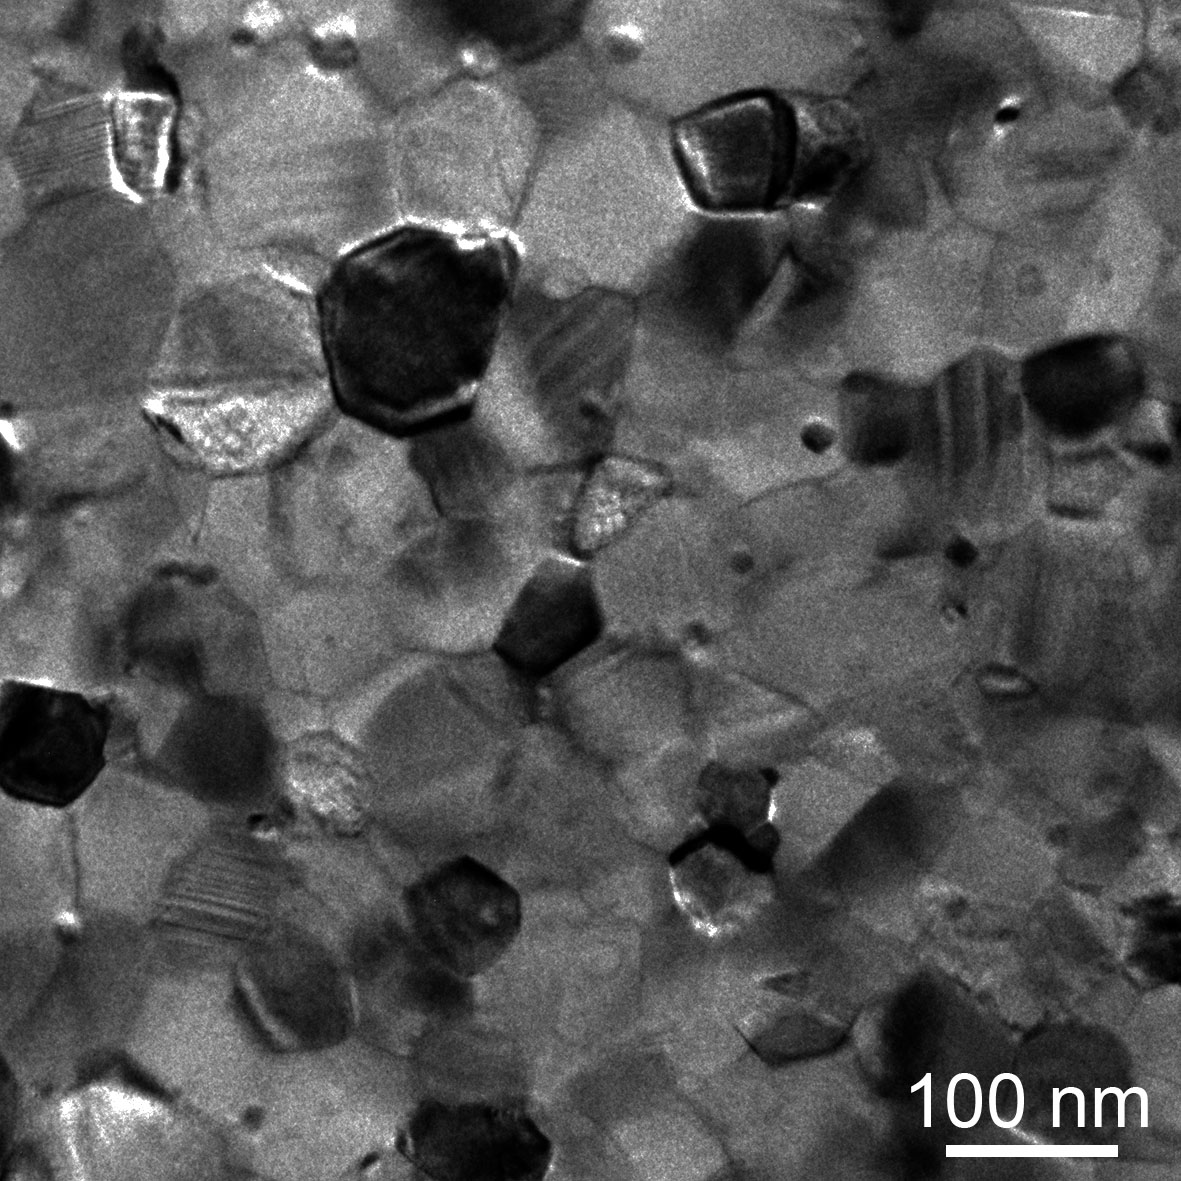
\includegraphics[scale=0.6]{img/TEM/Fig27c.jpg}}
\subfloat[Muestra a $800 ^\circ C$]{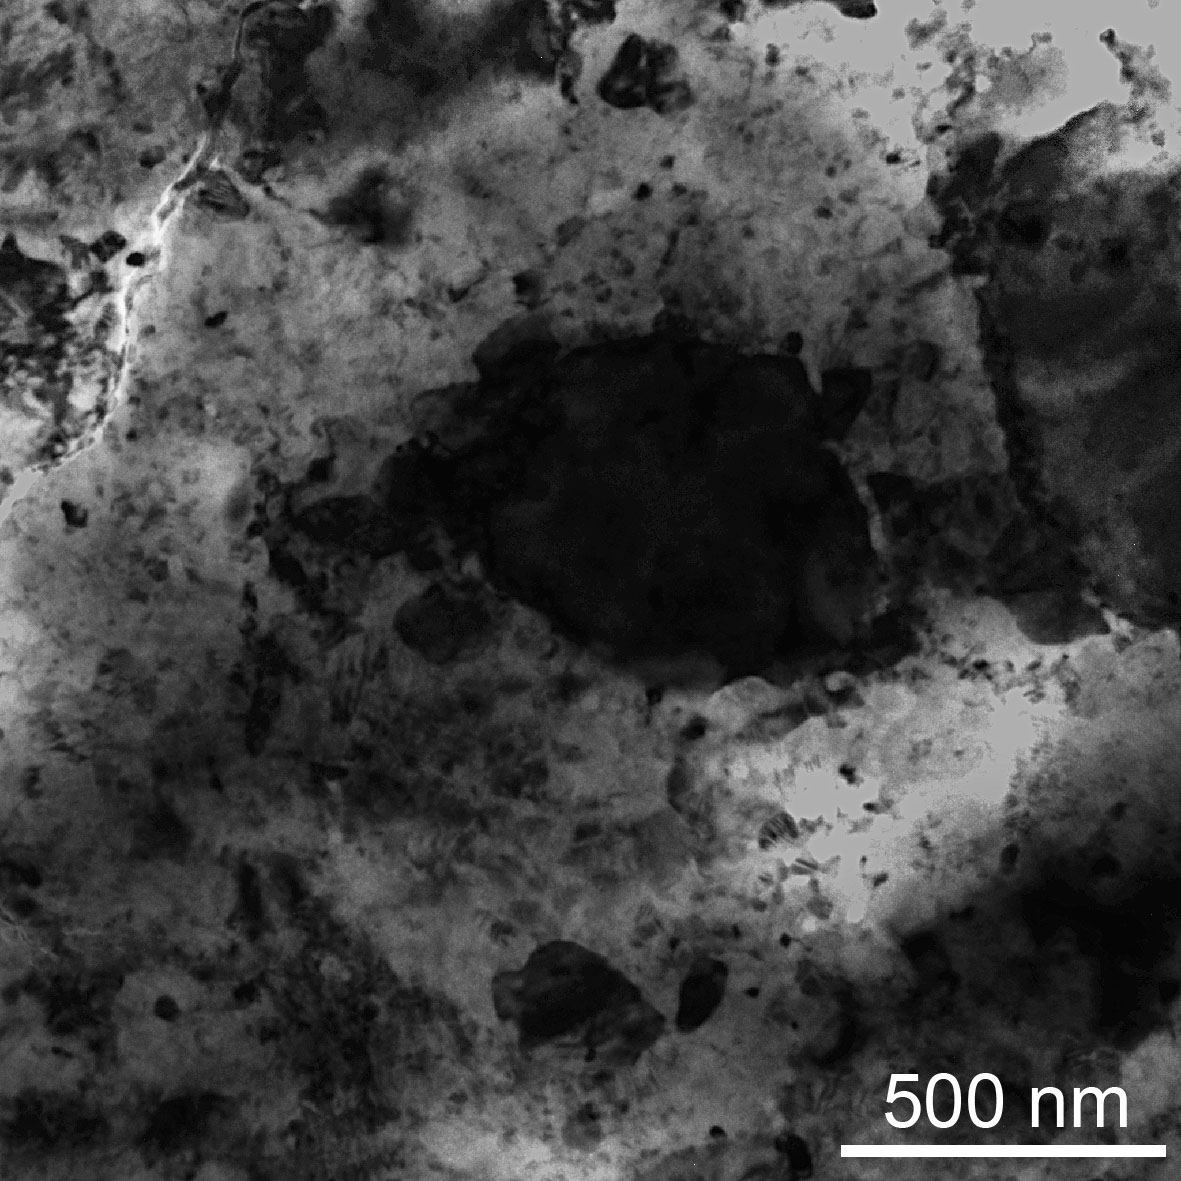
\includegraphics[scale=0.6]{img/TEM/Fig27d.jpg}}
\caption{Imágenes de TEM para las muestras ricas en $Ni$.}
\label{TEMNiRich}
\end{figure}

En la Figura \ref{TEMNiRich-PD}(a) se muestra el patrón de anillos de la lámina tratada a 500$^\circ C$, donde se puede observar que en esta muestra solo se encuentra la fase B2. En las muestras tratadas a mayor temperatura, la multiplicidad de fases presentes dificulta el análisis de los patrones de difracción de anillos. A esto se le suma la imposibilidad de obtener patrones de difracción de granos menores a los 100 $nm$. Debido a esto, en las muestras tratadas a mayor temperatura solo se podrá realizar un análisis de las fases de algunos de los granos que superen esta dimensión. En la Figura \ref{TEMNiRich-PD}(b) se puede observar un grano orientado de la muestra tratada a 600$^\circ C$ y su patrón de difracción, el cual corresponde al eje de zona $[111]$ de la fase B2. En la Figura \ref{TEMNiRich}(c), obtenida en la muestra tratada a 700$^\circ C$, se observan algunos granos con una morfología que puede asociarse a placas martensíticas, lo que correspondería a la presencia de la fase B19' en esta muestra. Además en la Figura \ref{TEMNiRich-PD}(c) se muestra un patrón de difracción de un grano que corresponde al eje de zona $[100]$ de la fase H, mostrando que esta fase dejó de ser un precipitado para constituirse en granos. En la Figura \ref{TEMNiRich-PD}(d) se puede observar que el tamaño de los granos de la fase H en la muestra tratada a 800$^\circ C$ supera los 500 $nm$.

\begin{figure}[H]
\centering
\subfloat[Muestra a $500 ^\circ C$]{\includegraphics[scale=0.6]{img/TEM/Fig28a.jpg}} 
\subfloat[Muestra a $600 ^\circ C$]{\includegraphics[scale=0.6]{img/TEM/Fig28b.jpg}} \\
\subfloat[Muestra a $700 ^\circ C$]{\includegraphics[scale=0.6]{img/TEM/Fig28c.jpg}}
\subfloat[Muestra a $800 ^\circ C$]{\includegraphics[scale=0.6]{img/TEM/Fig28d.jpg}}
\caption{Patrones de difracción TEM para las muestras ricas en $Ni$.}
\label{TEMNiRich-PD}
\end{figure}
\subsubsection{Transformación martensítica}
Para estudiar la transformación martensítica en el caso de las láminas ricas en $Ni$ se realizaron dos estudios: calorimetría diferencial de barrido y el método de resistividad por cuatro puntas.

Mediante el método de resistividad se logró detectar la transformación martensítica en la muestra tratada a $700 ^\circ C$ (ver Figura \ref{Res700}). Para determinar sus temperaturas se recurrió a un método gráfico, buscando la intersección de las rectas tangentes de los distintos puntos en la curva. Los puntos de intersección fueron buscados en forma analítica. Los valores son reportados en la Tabla \ref{TransformationPoints}.

\begin{figure}[H]
 	\centering
	\includegraphics[scale=0.3]{img/Resistance_700.png}
 	\caption{Curva de resistividad para la muestra tratada a $700 ^\circ C$, junto con las rectas usadas para determinar las temperaturas de transformación.}
	\label{Res700}
\end{figure}



\begin{table}[h]
\centering
\begin{tabular}{|c|c|}
\hline
Puntos de interés & Temperatura {[}$^\circ$ C{]} \\ \hline
$M_s$             & $56 \pm 2$                   \\ \hline
$M_f$             & $0 \pm 2$                    \\ \hline
$A_s$             & $18 \pm 2$                   \\ \hline
$A_f$             & $85 \pm 2$                   \\ \hline
\end{tabular}
\caption{Valores hallados para los principios y finales de ambas transformaciones.}
\label{TransformationPoints}
\end{table}

En las otras muestras, no fue posible definir dichas temperaturas. En la Figura \ref{Failures} se muestran estos resultados. Puede verse que en la muestras tratadas a $500 ^\circ C$ y a $800 ^\circ C$ las curvas en enfriamiento y en calentamiento permanecen casi siempre pegadas. Una leve diferencia se aprecia en la de  $500 ^\circ C$ entre aproximadamente $-70 ^\circ C$ y $20 ^\circ C$, pero no es suficiente para asegurar un cambio de fase. Por otra parte, en la lámina tratada a $600 ^\circ C$ hay un salto abrupto cerca de  $-45 ^\circ C$ y las curvas de calentamiento y enfriamiento lentamente se acercan llegando a $150 ^\circ C$. Sin embargo, por la presencia de ruido principalmente causado por inestabilidades debidas a los contactos a presión en estas láminas frágiles, no es posible establecer las temperaturas de transformación.

\begin{figure}[H]
\centering
\subfloat[Muestra a $500 ^\circ C$]{\includegraphics[scale=0.3]{img/Resistance_500.png}} \\
\subfloat[Muestra a $600 ^\circ C$]{\includegraphics[scale=0.3]{img/Resistance_600.png}}\\
\subfloat[Muestra a $800 ^\circ C$]{\includegraphics[scale=0.3]{img/Resistance_800.png}} 
\caption{Curvas medidas por el método de resistividad de cuatro puntas en las cuales no fue posible hallar en forma precisa las temperatura de transformación.}
\label{Failures}
\end{figure}


En la Figura \ref{DSCNiRich} se muestran las mediciones realizadas con el DSC luego de haberle sido sustraída la línea de base del equipo (el proceso se explica en la sección \ref{BaseLineAppendix}). En ninguna de las curvas es posible apreciar los picos correspondientes a la transformación de fase. Esto posiblemente se deba a la baja cantidad de masa que transforma, sumado al amplio rango de temperatura en la cual sucede la transformación de fase. Por ejemplo, en la muestra tratada a 700$^\circ C$, de acuerdo a la medición de resistividad por el método de cuatro puntas, la transformación sucede en un rango de aproximadamente 60$^\circ C$, mientras que la retransformación tiene lugar en un rango de 70$^\circ C$. Las causas de este amplio rango de transformación serán discutidas en la próxima sección.

\begin{figure}[H]

\noindent\makebox[\linewidth][c]{
	\subfloat[Enfriamiento, muestra tratada a $500 ^\circ C$]{\includegraphics[scale=0.13]{img/DSCNiRich/500NiRich}}
	\subfloat[Enfriamiento, muestra tratada a $600 ^\circ C$]{\includegraphics[scale=0.13]{img/DSCNiRich/600NiRich}}}\\
	
\noindent\makebox[\linewidth][c]{
\subfloat[Muestra tratada a $700 ^\circ C$]
{\includegraphics[scale=0.13]{img/DSCNiRich/700NiRich}}
}
	
 \caption{Curvas de DSC para muestras ricas en $Ni$ tratadas a diferentes temperaturas.}
\label{DSCNiRich}

\end{figure}

\newpage

\section{Discusión}
En esta sección se procederá a hacer un análisis de los resultados obtenidos, tanto individualmente como en su conjunto.

Primeramente se analizara la energía de activación de las láminas, contrastando los resultados obtenidos con estudios hechos en láminas de similares composiciones y métodos alternativos de producción.

Luego se analizarán los resultados de la difracción por rayos X y las imágenes de TEM para un análisis de cuales fueron las microestructuras y fases obtenidas luego de los tratamientos térmicos, para finalmente estudiar la influencia de estos factores en la transformación martensítica.

\subsection{Energía de activación}

Xiaoyang Yi et al \cite{XiaoyangYi2018} en 2018 determinaron la energía de activación, a través del método de Kissinger, para diversas composiciones de $NiTiZr$ en cintas producidas a través del método de solidificación rápida. Estos valores son reproducidos en la tabla \ref{XiaoyangYiValues}.

\begin{table}[H]
\centering
\begin{tabular}{|c|c|}
\hline
Composición & \begin{tabular}[c]{@{}c@{}}Energía de \\ activacion {[}kJ/mol{]}\end{tabular} \\ \hline
$Ni_{48,89}Ti_{40,50}Zr_{10,61}$ & 417,2 \\ \hline
$Ni_{48,71}Ti_{35,59}Zr_{15,70}$ & 432,9 \\ \hline
$Ni_{48,25}Ti_{31,26}Zr_{20,49}$ & 482,4 \\ \hline
$Ni_{47,95}Ti_{26,72}Zr_{25,33}$ & 465,8 \\ \hline
$Ni_{49,40}Ti_{19,96}Zr_{30,64}$ & 445,7 \\ \hline
\end{tabular}
\caption{Valores reportados por Xiaoyang Yi et al para la energía de activación para distintas composiciones en cinta.}
\label{XiaoyangYiValues}
\end{table}

Un año antes, Xiaoyang Yi et al \cite{XiaoyangYi2018_2} para cintas generadas por melt-spinning con una composición de $Ni_{49,6}Ti_{30,9}Zr_{19,5}$ determinó mediante el método de Kissinger $E_c = 449 \pm 5 kJ/mol$

Por otra parte, Malvasio en 2017 \cite{Malvasio}, en láminas delgadas obtenidas por deposición mediante magnetrón sputtering en la aleación binaria ($Ni_{54,2}Ti_{45,8}$), obtuvo una energía de activación de $E_c = 300 \pm 30 kJ/mol$ tanto por el método de Kissinger como por el método de Augis-Bennet.

En el presente trabajo se determinó la energía de activación de láminas delgadas de $NiTiZr$ producidas por magnetrón sputtering para la composición rica en $Ni$ ($Ni_{50,4}Ti_{30,8}Zr_{18,9}$) y se obtuvieron valores de $E_c = 420 \pm 30$ kJ por el método de Kissinger y de $E_c = 410 \pm 30$ kJ por el método de Augis-Bennet. Si bien estos valores son levemente inferiores a los determinados por Xiaoyang Yi et al., son notoriamente mayores que los obtenidos en la aleación binaria. La leve diferencia entre los valores determinados en este trabajo con los valores obtenidos por Xiaoyang Yi et al. (\cite{XiaoyangYi2018_2} y \cite{XiaoyangYi2018}) puede ser entendida teniendo en cuenta las diferentes técnicas de producción. Estas diferencias en los valores de la energía de activación causado por los procesos de producción, ya fueron mostrados en la aleación binaria \cite{Chen1999}.

\subsection{Microestructuras y fases presentes}
En las siguientes secciones se listan las fases halladas y los tamaños de grano para cada composición, contrastando con los resultados obtenidos por otros autores.
\subsubsection{Pobre en $Ni$}
\label{DPobreNi}

En la Tabla \ref{PhasesNiPoor} se reportan las distintas fases halladas y los tamaños de grano observados para los distintos tratamientos térmicos en las muestras con composición pobre en $Ni$ ($Ni_{46}Ti_{33,2}Zr_{20,8}$).

\begin{table}[H]
\centering
\begin{tabular}{|c|c|c|}
\hline
\begin{tabular}[c]{@{}c@{}}Temperatura del\\ tratamiento $[^\circ C]$\end{tabular} & Fases halladas & Tamaño de grano {[}$nm${]} \\ \hline
500 & B2 - $Ti_2Ni$                      & 10 a 50             \\ \hline
600 & B2 - $Ti_2Ni$ - $NiZr$ - $\lambda$ & 110 a 140 - 10 a 30 \\ \hline
700 & B2 - $Ti_2Ni$ - B19'               & $\sim$ 90           \\ \hline
800 & B2 - $Ti_2Ni$ - $NiZr$               & 20 a 130            \\ \hline
\end{tabular}
\caption{Fases halladas y tamaño de grano para cada tratamiento térmico en la deposición pobre en $Ni$.}
\label{PhasesNiPoor}
\end{table}

En todas estas muestras se observaron la fase austenítica B2 y la fase $Ti_2Ni$, lo cual es esperable ya que ambas son fases de equilibrio para esta composición. También es posible que esté presente la fase $Ti_4Ni_2O$, pero como fue explicado en la sección \ref{Ti2Ni}, resulta difícil de diferenciarla de la fase $Ti_2Ni$ mediante rayos X, ya que ambas fases presentan estructuras similares, con una leve diferencia en el parámetro de red ocasionado por la presencia del $O$ en la estructura. Esta suposición es apoyada por el hecho que las muestras presentaban una leve capa de óxido superficial luego de los tratamientos térmicos, en especial en las muestras tratadas a mayor temperatura. Además, es necesario notar que los picos de rayos X correspondientes a la fase $Ti_2Ni$, en las muestras tratadas a $700 ^\circ C$ y $800 ^\circ C$, presentan un ancho superior a los picos de las otras fases. Dicho ensanchamiento podría deberse a variaciones del parámetro de red ocasionadas por la presencia heterogénea de $Zr$, en detrimento del $Ti$ en las estructuras de las fases $Ti_2Ni$ y $Ti_4Ni_2O$. Por otro lado, la presencia de las fases $\lambda$ y $NiZr$ en la muestra tratada a $600^\circ C$, concuerda con lo observado en el trabajo de Kim {\it et al.} \cite{HeeYoungKim2009}, donde ambas fases son reportadas en las láminas producida por sputtering, con una composición de $Ni_{49,5} Ti_{30,8} Zr_{19,7}$, tratada a la misma temperatura. Vale aclarar que estas fases si bien están presentes, representan proporciones minoritarias. Es importante notar que en el trabajo Kim {\it et al.} no se observó la fase $Ti_2Ni$ para ninguno de los tratamientos térmicos. Esto puede deberse a que la composición es cercana al $50$ $\%$ de $Ni$. En el trabajo de Yi {\it et al.} en 2018 \cite{XiaoyangYi2018} se estudiaron láminas producidas por melt-spinning y en su composición de $Ni_{48,3}Ti_{31,2}Ni_{20,5}$ sólo se observa la fase $\lambda$ como precipitado luego de los tratamientos a 600$^\circ C$, 700$^\circ C$ y 800$^\circ C$. Dicha discrepancia probablemente se deba a la forma distinta de generar la aleación. Por último la presencia de la fase $B19^{\prime}$ en la muestra tratada a $700$ $^\circ C$ será discutido en la sección \ref{disNipoor}.


Los tamaños de grano aumentan, como es esperado, al aumentar la temperatura del tratamiento térmico, manteniéndose sin embargo siempre menores a los $200$ $\mu m$. Estos tamaño de granos son similares a los informados por Sawaguchi {\it et al.} en 2004 \cite{Sawaguchi2004}, informe en el cual estudió láminas delgadas producidas por sputtering con una composición con menor porcentaje de $Zr$ ($Ni_{49,7} Ti_{35,0} Zr_{15,4}$). Además, en dicho trabajo, se muestra una distribución bimodal de tamaño de grano para la fase $\lambda$ y $B2$  que varía dependiendo del tratamiento térmico, de manera similar a la distribución bimodal entre la fase $B2$ y $Ti_2 Ni$ observada en la muestra tratada a $600 ^\circ C$.} 

\subsubsection{Rica en $Ni$}

En la Tabla \ref{PhasesNiRich} se resumen las distintas fases halladas y los tamaños de grano observados para cada una de las muestras ricas en $Ni$ ($Ni_{50,4}Ti_{30,8}Zr_{18,9}$) sometidas a un tratamiento térmico. Este caso en particular se encuentra menos estudiado que su contraparte pobre en $Ni$. Por este motivo, se hacen también comparaciones con la aleación $NiTiHf$, que ha sido más estudiada y presenta estructuras similares \cite{Santamarta2013}.


\begin{table}[H]
\centering
\begin{tabular}{|c|c|c|}
\hline
\begin{tabular}[c]{@{}c@{}}Temperatura del\\ tratamiento $[^\circ C]$\end{tabular} & Fases halladas & Tamaño de grano {[}$nm${]} \\ \hline
500 & B2                         & $\sim$ 70  \\ \hline
600 & B2 - $Ti_2Ni$              & $\sim$ 90  \\ \hline
700 & B2 - $Ti_2Ni$ - B19' - H   & $\sim$ 115 \\ \hline
800 & B2 - $Ti_2Ni$ - H - $NiZr$ & 50 a 500      \\ \hline
\end{tabular}
\caption{Fases halladas para cada tratamiento térmico en la deposición rica en $Ni$.}
\label{PhasesNiRich}
\end{table}

Al igual que en la sección anterior, en todas las muestras se aprecia la fase B2, y en todas, exceptuando aquella tratada a menor temperatura, la fase $Ti_2Ni$. Sin embargo, a diferencia de las muestras pobre en $Ni$, esta última fase no es una fase de equilibrio del sistema (ver Figura \ref{PhaseDiagram} en la Sección \ref{PhaseDiagramSection}), con lo cual es probable que se trate de la fase $Ti_4Ni_2O$. Cómo en el caso anterior, esta hipótesis se basa en que también se observó una capa superficial de óxido en estas muestras, luego de los tratamientos térmicos. A pesar de esto, no es posible asegurar que la fase $Ti_2Ni$ no este presente, ya que tanto la fase $NiZr$ como la fase H pueden sustraer $Ni$ de la fase matriz, produciendo que su composición final sea pobre en $Ni$ y por tanto precipitando la fase $Ti_2Ni$.

La presencia de la fase H en las muestras tratadas a $700$ $^\circ C$ y $800$ $^\circ C$ es destacable, ya que cuando esta fase se encuentra en forma de nanoprecipitados coherente con la fase matríz endurece la estructura del material, lo cual la hace menos propensa a sufrir una deformación plástica. La estructura de esta fase fue descripta en el 2013 en los trabajos \cite{Santamarta2013} y \cite{Yang2013}, y los estudios de los tratamientos térmicos necesarios para obtener nanoprecipitados de esta fase y las propiedades de estas aleaciones producidas por método convencionales se pueden encontrar en los trabajos \cite{Evirgen2013} \cite{Evirgen2014} \cite{Evirgen2016} \cite{Perez-Sierra2016} \cite{Evirgen2018} y \cite{Bigelow2019}. Sin embargo, no existe en la bibliografía estudio de láminas delgadas de $NiTiZr$ ricas en $Ni$ producidas por sputtering, por lo cual no es posible realizar una comparación directa de resultados obtenidos.

La presencia de la fase B19' en la muestra tratada a $700$ $^\circ C$ a temperatura ambiente será discutida en la sección \ref{disNirich}.

En cuanto a la microestructura, se puede observar un crecimiento del tamaño de grano mayor con el aumento de la temperatura de los tratamientos térmicos, en comparación con la aleación pobre en $Ni$. Además se observa que los tratamientos térmicos de $700$ $^\circ C$ y $800$ $^\circ C$ durante 1 hora no son eficientes para obtener precipitados nanométricos de la fase H en el interior de los granos de la fase B2, ya que se observan granos de la fase H mayores a los 100 $nm$.


\subsection{Transformación martensítica}
\label{TransfomacionDiscusion}

En las siguientes secciones se discutirán cuales son los factores, dentro del marco termodinámico, que produjeron que las temperaturas de transformación se encuentren por debajo de los valores esperados, así como las dificultades asociadas a la determinación de la transformación martensítica.

%Con el objetivo de medir las temperaturas asociadas a la transformación martensítica ($M_s$, $A_s$, $M_f$ y $A_f$) para ambas tandas se midió la variación en el flujo de calor usando la técnica de calorimetría diferencial de barrido. En las muestras pobre en $Ni$ adicionalmente pudo ser realizada la medición de la resistividad en función de la temperatura por el método de cuatro puntas. 
%
%Las temperaturas asociadas a la transformación pudieron ser determinadas para la muestra rica en $Ni$ tratada a $700^\circ C$. En el resto de las muestras no pudieron ser determinadas por ser mucho menores a la temperatura ambiente o, posiblemente, ni siquiera suceder en ciertos casos.


\subsubsection{Pobre en $Ni$}
En las muestras de esta deposición no fue posible observar, mediante las mediciones de DSC, un cambio en el flujo de calor que permitiese determinar el principio y el final de los cambios de fase. Esto pudo ser causado por dos factores: la extensión de la transformación en un amplio rango de temperaturas, ensanchando el pico de transformación, lo cual hace difícil diferenciarla de la línea de base del DSC y una baja cantidad de masa transformando. A estas dificultades relacionadas con las mediciones de DSC, se le sumó la imposibilidad de implementar resistividad de cuatro puntas, debido a la fragilidad de las muestras.


A pesar de esto, puede afirmarse que las temperaturas de transformación son menores a la temperatura ambiente, ya que mediante las imágenes de TEM y la difracción de rayos X, sabemos que las muestras se encuentran principalmente en fase B2 (Austenita). La excepción es la muestra tratada a $700^\circ C$, ya que en ella se observan tanto la fase B2 como la B19'. A partir de este hecho se puede concluir que para esta muestra las temperaturas de transformación son cercanas a la temperatura ambiente.

El motivo de que la temperatura de equilibrio $T_0$ sea menor que la temperatura ambiente se debe principalmente a la composición. La presencia de otras fases remueve parcialmente $Zr$ de la fase matriz, evitando así que tenga el efecto de aumentar $T_0$ sobre la temperatura ambiente (dicho efecto se muestra en la Figura \ref{ZrDependence}). Aparte de esto, en particular la presencia de las fases $(Ti, Zr)_2 Ni$ y $(Ti, Zr)_4 N_2O$ sacan mayor contenido de $Ti$ y de $Zr$ que de $Ni$ de la fase matriz. Esto probablemente implique que la fase matriz termina siendo rica en $Ni$, bajando las temperaturas de transformación, ya que como se muestra en la Figura \ref{NiDependence}, a mayor porcentaje de $Ni$, menores temperaturas de transformación.

\begin{figure}[H]
 	\centering
	\includegraphics[scale=0.7]{img/MsZrDependence.jpeg}
 	\caption{Efecto del porcentaje de $Zr$ en las temperaturas de transformación en la aleación $NiTiZr$. }
	\label{ZrDependence}
\end{figure}

\begin{figure}[H]
 	\centering
	\includegraphics[scale=0.7]{img/MsNiDependence.png}
 	\caption{Efecto del porcentaje de $Ni$ en las temperaturas de transformación en la aleación $NiTi$.}
	\label{NiDependence}
\end{figure}


Por otra parte, el bajo tamaño de grano presente en las microestructuras producen que la transformación se extienda en un rango amplio de temperatura y que las temperaturas de transformación desciendan. Esto puede entenderse a partir de la Ecuación \ref{GibbsEnergyEquation}:
\begin{equation*}
	- \Delta G_{q}^{A \leftrightarrow M} \geq W_{elast} + W_{fric}
\end{equation*} 
Al disminuir el tamaño de grano, aumenta el trabajo elástico necesario tanto para introducir el primer núcleo de martensita como para que la transformación avance. Para poder realizar este trabajo el sistema necesita una mayor energía libre $\Delta G_{q}$, lo cual se logrará con un mayor sobreenfriamiento, bajando efectivamente la temperatura a la cual comienza la transformación ($M_s$) y extendiendo el rango de transformación (distancia entre $M_s$ y $M_f$).

La influencia del tamaño de grano sobre la $M_s$ fue estudiado por Waitz en 2007 y 2008 \cite{Waitz2007}\cite{Waitz2008}. En estos trabajos se marca incluso que la transformación se suprime completamente con tamaños de granos menores a 50 $nm$. Viendo las imágenes de la sección \ref{TemNiPoorResults}, se observa que todas las muestras tienen granos con tamaños menores a 50 $nm$, y, particularmente, en la muestra tratada a $500^\circ C$ no se observan granos superiores a dicho tamaño. Esto explicaría porque en esta muestra no se observa transformación a pesar de que en los rayos X y en las imágenes obtenidas por TEM la fase mayoritaria es la B2.

Por último, es destacable que la presencia de las fases adicionales disminuye el porcentaje de las fases B2 y B19', fases involucradas en la transformación martensítica. Este menor porcentaje de fase que transforma, sumado a que la masa de las láminas delgadas es pequeña, produce que los picos asociados a la transformación martensítica en las mediciones de calorimetría diferencial de barrido sean más chicos, y por lo tanto, más difíciles de apreciar. Por esta causa, sumado al amplio rango de temperatura donde sucede la transformación ocasionado por el pequeño tamaño de grano, es que no pudieron ser apreciadas las temperaturas de transformación en la muestra tratada a $700^\circ C$, a pesar de saber que se trabajó en un rango de temperaturas en el cual la transformación sucede.


\subsubsection{Rica en $Ni$}

El análisis de las muestras de esta composición es similar al análisis de las muestras pobres en $Ni$, con el agregado que en este caso se realizó la medición de resistividad por el método de cuatro puntas.

En este caso, en la muestra tratada a $700 ^\circ C$ se pudo observar una transformación de fase, apreciable únicamente en la medición de la resistividad. Las temperaturas de transformación halladas en este caso ($M_s = 56 ^\circ C$, $M_f = 0 ^\circ C$, $A_s = 18 ^\circ C$, $A_f = 86 ^\circ C$) , son coincidentes con el hecho que esta es la única muestra de la tanda rica en $Ni$ que presenta la fase B19' a temperatura ambiente. La transformación martensítica se produce en un rango de $56 ^\circ C$, mientras que la austenítica en un rango de casi $68^\circ C$. La causa de esta amplitud es atribuible al bajo tamaño de grano,el cual hace necesario un mayor trabajo elástico tanto para iniciar como para completar la transformación, cómo ya fue descripto en la sección anterior. Este amplio rango de temperatura en el cual sucede la transformación y la presencia de fases adicionales que no transforman, son justamente los causantes de que este cambio de fase no pueda ser apreciado en la calorimetría diferencial de barrido.

En cuanto a las otras muestras, no fue posible determinar con precisión la transformación ni por DSC ni por la técnica de resistividad por cuatro puntas. Pero al igual que las muestras con composición pobre en $Ni$, se pudo determinar que la fase B2 está presente a temperatura ambiente. Nuevamente esto indica que si existe la transformación, esta sucede a una temperatura menor a la ambiente. Este hecho está relacionado con un corrimiento hacia menores temperatura de la $T_0$, debido al empobrecimiento de $Zr$ y $Ti$ en la fase matriz, caudado por la precipitación de $(Ti,Zr)_2 Ni$, de la fase $NiZr$ y de la fase H ($Ni_{0,5} Ti_{0,167} Zr_{0,333}$) y al sobreenfiamiento necesario para vencer el trabajo elástico necesario para producir la transformación.

Queda pendiente realizar un análisis de DSC de la muestra tratada a $800 ^\circ C$, medición que no pudo ser hecha debido a la pandemia de COVID-19. Sin embargo, en vista que en ninguna de las otras muestras se apreció un cambio de fase por medio de DSC, es poco probable que dicha medición arrojase nueva información.

\newpage
\section{Conclusión}
En el presente trabajo se logró obtener láminas delgadas de $NiTi$ con un agregado de $Zr$, tanto en las llamadas composiciones ricas en $Ni$ como en aquellas pobres en $Ni$. El $Zr$ fue introducido con la intención de aumentar las temperaturas de transformación y así estudiar materiales con memoria de forma de alta temperatura. Particularmente se prestó atención a la energía de activación del proceso de cristalización y a las microestructuras obtenidas y su relación con la transformación de fase martensítica. 

Para ello se realizaron dos deposiciones en las que se obtuvieron 12 láminas delgadas de aproximadamente 8 $mm$ x 25 $mm$ en estado amorfo por la técnica de co-sputtering, utilizando simultáneamente un blanco de $Ti$, uno de $Ni$ y uno de $Zr$. Mediante un análisis por EDS-SEM, se logró determinar que las muestras ricas en $Ni$ tenían una composición de 50,4 at\% $Ni$, 30,8 at\% $Ti$ y 18,9 at\% $Zr$, mientras que las muestras pobres en $Ni$ tenían una composición de 46 at\% $Ni$, 33,2 at\% $Ti$ y 20,8 at\% $Zr$.

Posteriormente se estudió la energía de activación del proceso de cristalización de las muestras ricas en $Ni$. Para dicho estudio se midió el flujo de calor para las velocidades de calentamiento 5$^\circ C/min$, 10$^\circ C/min$, 20$^\circ C/min$, 30$^\circ C/min$ y 50$^\circ C/min$, y empleando los modelos de Augis-Bennet y de Kissinger se obtuvieron los valores de (410 $\pm$ 30) $kJ$ y (420 $\pm$ 30) $kJ$, respectivamente. Valores coincidentes entre sí, dentro del margen de error, y comparables con los informados por otros autores.

Las muestras de ambas deposiciones fueron tratadas térmicamente por una hora a $500^\circ C$, $600^\circ C$, $700^\circ C$ y $800^\circ C$ en una atmósfera controlada de $Ar$, para estudiar luego los efectos de los tratamientos en la microestructura y su relación con las propiedades de la transformación martensítica.

Para determinar las fases presentes y los tamaños de grano, las muestras tratadas fueron sometidas a estudios de difracción por rayos X y obtención de imágenes por TEM. Para las muestras con composición pobre en $Ni$ tratadas a $500$ $^\circ C$ se hallaron las fases B2 y precipitados de la fase $(Ti, Zr)_2Ni$ (o posiblemente $(Ti, Zr)_4Ni_2O$), mientras que para la muestra tratada a $600$ $^\circ C$ además se observó las fases $\lambda$ y $NiZr$. Dicha fase $\lambda$ no fue observada en las muestras tratadas a $700$ $^\circ C$ y $800$ $^\circ C$. Finalmente en la muestra tratada a $800$ $^\circ C$ se observó, además de las fases B2 y $(Ti, Zr)_2Ni$, la fase $NiZr$. La microestructura de estas muestras estuvo caracterizada por el tamaño de grano siempre menor a 200 $nm$ y mostrando un leve crecimiento con el aumento de la temperatura de los tratamientos térmicos. Por el otro lado, en las muestras con composición rica en Ni, la muestra tratada a $500$ $^\circ C$ solo mostró la fase B2, mientras que la precipitación de la fase $(Ti, Zr)_2Ni$ ((o posiblemente $(Ti, Zr)_4Ni_2O$) se observó en todas las muestras tratadas a mayor temperatura. La fase H fue observada en las muestras de $700$ $^\circ C$ y $800$ $^\circ C$, mientras que la fase $NiZr$ solo se observó en la muestra tratada a $800$ $^\circ C$. La microestructura de las muestras de esta composición se caracterizó por un crecimiento mayor del tamaño con la temperatura de los tratamientos térmicos, donde las muestras tratadas a $500$ $^\circ C$ mostró una distribución de granos con un valor medio de  70 $nm$, hasta alcanzar tamaños cercanos a 500$nm$ en la muestra tratada a $800$ $^\circ C$.

Con el objetivo de medir las propiedades de la transformación de fase, se realizaron las mediciones de calorimetría diferencial de barrido y resistividad por el método de cuatro puntas, pudiéndose implementar esta última sólo para las muestras ricas en $Ni$. En particular, en la muestra con composición rica en $Ni$ tratada a $700^\circ C$, fue posible determinar las temperaturas asociadas a la transformación martensítica mediante la técnica de resistividad ($M_s=56^\circ C$, $M_f=0^\circ C$, $A_s=18^\circ C$, $A_f=85^\circ C$, en todos los casos con una incerteza de $2^\circ C$). Mientras que en la muestra con composición pobre en $Ni$ tratada a $700^\circ C$ solamente se pudo determinar que su transformación de fase sucede a temperaturas cercanas a la ambiente, indicado por la presencia de la fase B19'. En el resto de las muestras, se pudo determinar que la transformación, si sucede, lo hace a temperaturas menores a la ambiente, ya que contienen una presencia mayoritaria de fase B2 a dicha temperatura.

Los corrimientos de las temperaturas de transformación hacia valores menores, pudo ser entendido por el descenso de la temperatura de equilibrio $T_0$, ocasionado por la pérdida de $Zr$ y $Ti$ en la fase matriz, debido a la presencia de las fases $(Ti,Zr)_2 Ni$, $\lambda$ y $NiZr$ para las muestras con composición pobres en $Ni$, mientras que el mismo razonamiento puede ser aplicado para las muestras ricas en $Ni$, debido a la presencia de las fases $(Ti,Zr)_2 Ni$, H y $NiZr$. A esta causa, se le suma la presencia de microestructuras caracterizadas por granos del orden de cien nanómetros, generando la necesidad de un sobreenfriamiento mayor. Dicho sobreenfriamento era necesario para poder obtener la energía libre de Gibbs suficiente para que el sistema pueda realizar el trabajo elástico necesario para inducir la transformación martensítica. Siguiendo la misma línea de pensamiento, estas microestructuras de granos muy pequeños produjeron que la transformación esté extendida en un rango de temperatura amplio. Este hecho junto con la caída del porcentaje de masa que transforma dentro de las muestras, debido a la presencia de otras fases, ocasionaron la imposibilidad de detectar la transformación por el método de calorimetría diferencial de barrido.

En base a lo visto en este trabajo, se propone en futuros estudios la optimización de los tratamientos térmicos para seleccionar la microestructura con precipitados nanométricos en el interior de los granos de la fase matriz, de modo de endurecerla sin cambiar drásticamente su estequiometría. Se sugiere, en particular, continuar con el estudio de las láminas ricas en $Ni$, ya que está demostrado la eficiencia de la fase H para endurecer la fase matriz en las aleaciones producidas por métodos convencionales, sin embargo no hay estudios en láminas delgadas de dicha composición en la bibliografía.


% You can choose a citation style, 'plain' is the default
% See:
% https://www.overleaf.com/learn/latex/Bibtex_bibliography_styles
\newpage
\nocite{*} 
\bibliographystyle{plain}
\bibliography{Referencias}

\newpage
\appendix
\section{Apéndice}
\label{Appendix}
\subsection{Restado de la línea base en las mediciones de DSC}
\label{BaseLineAppendix}

Para correctamente analizar las curvas obtenidas en el DSC, era necesario a las mediciones sustraerles la medición de la línea base. Para realizar esto, primero cada curva fue dividida en su parte de enfriamiento y su parte de calentamiento. Lo mismo fue hecho con la medición de la línea base. Para realizar la resta una vez hecha esta división, era necesario que ambas curvas tuvieran exactamente los mismos puntos en el eje de la temperatura. Para que esto suceda, todas las mediciones fueron unidas por splines lineales
y luego se procedió a una interpolación. No se considera que esto haya introducido un error apreciable, ya que la medición presenta poco ruido y los puntos originales son muy cercanos entre sí.

En la Figura \ref{MeasureExample} se muestra como ejemplo una medición obtenida en DSC y en la Figura \ref{BaseLine} la medición de la línea base correspondiente.

\begin{figure}[H]
	\centering	
	\includegraphics[scale=0.3]{img/500NiPoorExample}
	\caption{Medición de DSC para la muestra pobre en $Ni$ tratada a 500 $^\circ C$.}
	\label{MeasureExample}
\end{figure}

\begin{figure}[H]
	\centering
	\includegraphics[scale=0.3]{img/BaseLine}
	\caption{Medición de DSC para la línea de base.}
	\label{BaseLine}
\end{figure}

En la Figura \ref{Comparison} se muestran la medición original, la línea base y la diferencia entre ambas, para el calentamiento.

\begin{figure}[H]
	\centering
	\includegraphics[scale=0.2]{img/NiPoorHeatingExample}
	\caption{Comparación entre medición, línea de base y su diferencia.}
	\label{Comparison}
\end{figure}


Todo este proceso fue reaizado en Python 3.7, usando las librerías \textit{SciPy} y \textit{Numpy}.

\subsection{Obtención de picos para energía de activación}

Para obtener en forma correcta el máximo de los picos en las mediciones de DSC, en lugar de sustraer la línea base se procedió a unir con una recta los puntos de inicio y fin de cada pico, y luego restar dicha recta de la medición original. Esta decisión se tomo debido a que en un intervalo acotado, una recta es una muy buena aproximación de la línea de base.

\end{document}

% Have fun!
% -fons

% http://www2.washjeff.edu/users/rhigginbottom/latex/resources/symbols.pdf
